\documentclass[master]{BYUPhys}
% % These packages typeset the thesis with Times Roman font
% \usepackage[T1]{fontenc}
% \usepackage{textcomp}
% \usepackage{mathptmx}

%I love these packages.
\usepackage{amsmath}
\usepackage{amssymb}



% Allow the inclusion of graphics
\usepackage{graphicx}
\usepackage{subfig}

% The fancyhdr package allows you to easily customize the page header.
% The settings below produce a nice, well separated header.
\usepackage{fancyhdr}
  \fancyhead{}
  \fancyhead[LO]{\slshape \rightmark}
  \fancyhead[RO,LE]{\textbf{\thepage}}
  \fancyhead[RE]{\slshape \leftmark}
  \fancyfoot{}
  \pagestyle{fancy}
  \renewcommand{\chaptermark}[1]{\markboth{\chaptername \ \thechapter \ \ #1}{}}
  \renewcommand{\sectionmark}[1]{\markright{\thesection \ \ #1}}

% The caption package allows you to change the formatting of figure captions.
% The commands here change to the suggested caption format: single spaced and a bold tag
\usepackage[margin=0.3in,labelfont=bf,labelsep=none]{caption}
 \DeclareCaptionFormat{suggested}{\singlespace#1#2 #3\par\doublespace}
 \captionsetup{format=suggested}


% The cite package cleans up the way citations are handled.  For example, it
% changes the citation [1,2,3,6,7,8,9,10,11] into [1-3,6-11].  If your advisor
% wants superscript citations, use the overcite package instead of the cite package.
\usepackage{cite}

% The makeidx package makes your index for you.  To make an index entry,
% go to the place in the book that should be referenced and type
%  \index{key}
% An index entry labeled "key" (or whatever you type) will then
% be included and point to the correct page.
\usepackage{makeidx}
\makeindex

% If you have a lot of equations, you might be interested in the amstex package.
% It defines a number of environments and macros that are helpful for mathematics.
% We don't do much math in this example, so we haven't used amstex here.

% The hyperref package provides automatic linking and bookmarking for the table
% of contents, index, equation references, and figure references.  It must be
% included for the BYU Physics class to make a properly functioning electronic
% thesis.  It should be the last package loaded if possible.
%
% To include a link in your pdf use \href{URL}{Text to be displayed}.  If your
% display text is the URL, you probably should use the \url{} command discussed
% above.
%
% To add a bookmark in the pdf you can use \pdfbookmark.  You can look up its usage
% in the hyperref package documentation
\usepackage[bookmarksnumbered,pdfpagelabels=true,plainpages=false,colorlinks=true,
            linkcolor=black,citecolor=black,urlcolor=blue]{hyperref}
\urlstyle{rm}
% ------------------------- Fill in these fields for the preliminary pages ----------------------------
%
% For Senior and honors this is the year and month that you submit the thesis
% For Masters and PhD, this is your graduation date
  \Year{2015}
  \Month{June}
  \Author{James Lawrence Archibald II}

% If you have a long title, split it between two lines using the \\ command.
% A multiple line title should be an "inverted pyramid" with the top line(s) longer than the bottom.
  \Title{Construction of a 408 nm Laser System \\ for use in Ion Interferometry}

% Your research advisor
  \Advisor{Dallin S. Durfee}

% The text of your abstract
  \Abstract{
We discuss the construction of a 408 nm laser system for use in a $^{87}$Sr+ ion interferometer. This work reports progress towards driving stimulated Raman transitions between the $F=4$ and $F=5$ $^2$S$_{1/2}$ states of $^{87}$Sr$+$ using the $^2$P$_{3/2}$ state as the intermediate state.

The scope of this work is limited to the construction of a laser system that is intended to drive the stimulated Raman transitions in our ion interferometer experiment (also known as the 408 nm 5GHz detuned laser system).
This work also includes a discussion of the relevant theory along with some calculations about the transition rates and power levels involved in getting the experiment to work. 

We will also provide a brief summary of the ion interferometer and a discussion of its place among related experiments. 
}

 \Keywords{Sr, ion interferometer, photon rest mass, laser, AOM}

% Acknowledge those who helped and supported you
  \Acknowledgments{Camille has been a wonderful support. 
  }

\fussy
\DeclareMathOperator{\erf} {erf}


\begin{document}
\frontmatter

\makepreliminarypages

\singlespace

\tableofcontents
\clearemptydoublepage

\listoffigures
\clearemptydoublepage

\doublespace


\newcommand{\includeorput}[1]{\include{#1}} %\newcommand{\includeorput}[1]{\input{#1}}
\mainmatter


\chapter{Background}
In this chapter, we discuss the overall experiment of which the 408 nm 5 GHz detuned laser system is a part. We will give a detailed summary of the preparation the atoms undergo before they are exposed to our laser system. We will also attempt to sensibly contextualize the ion interferometer vis-\`a-vis other physics experiments. 

\section{Ion Interferometer Basic Overview}
The ion interferometer uses a Mach-Zehnder configuration, which refers to the fact that it relies on splitting and recombining the interfering beam of atoms. See Fig.\ \ref{mach-zehnder-fig}. 


\begin{figure}
\centerline{
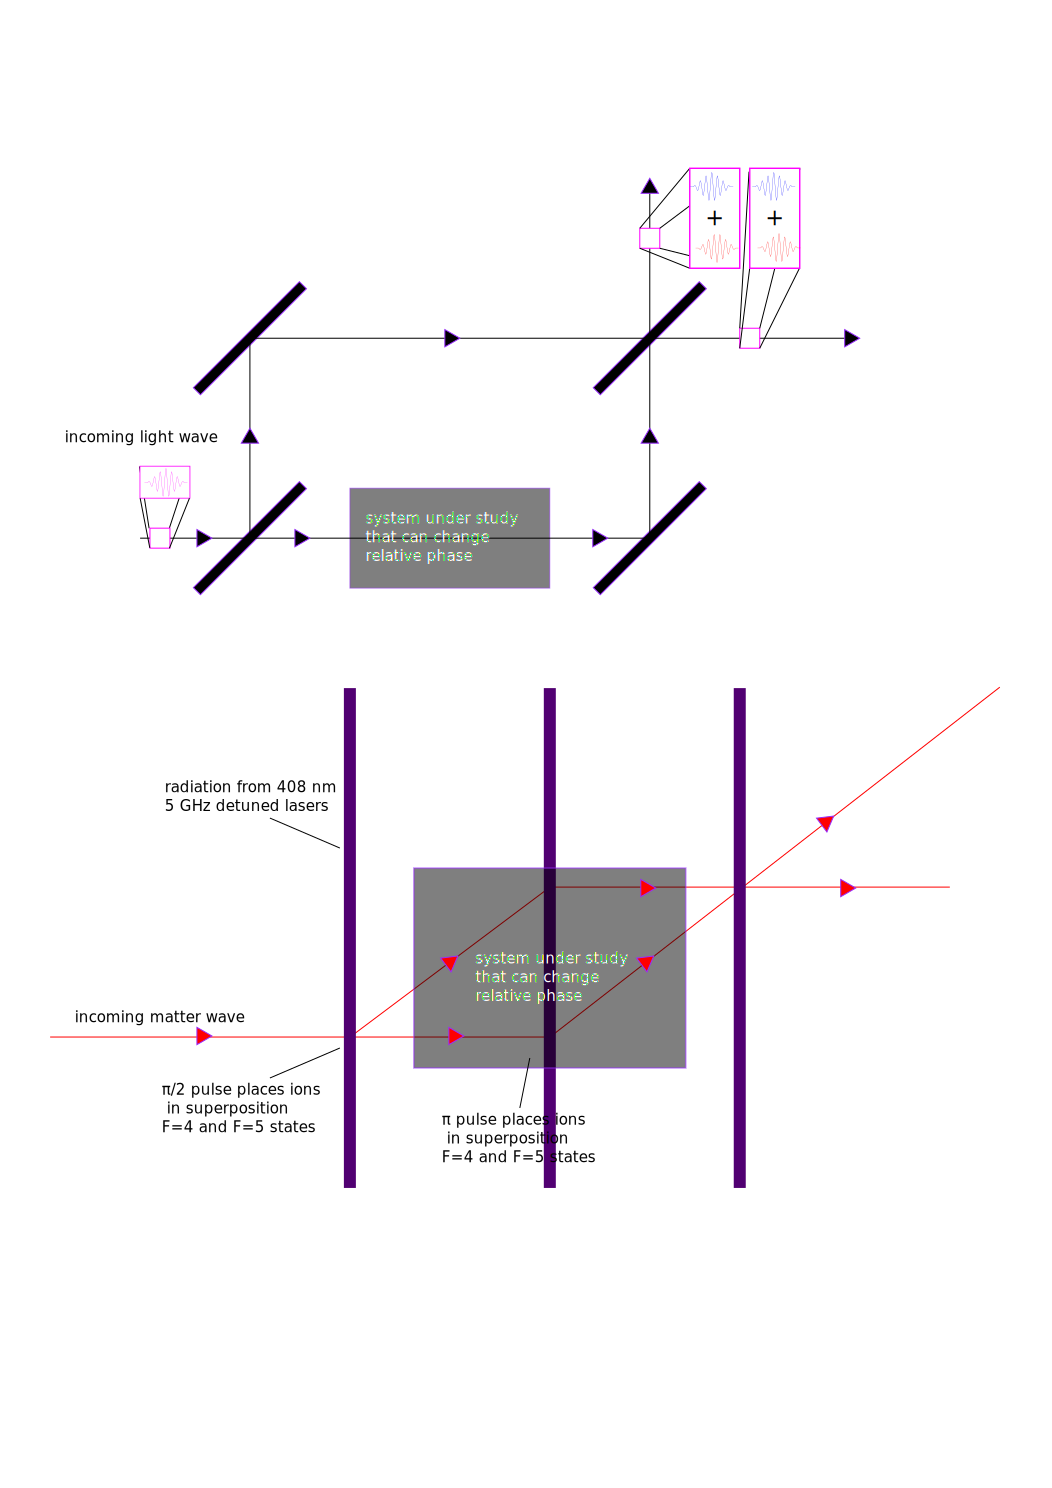
\includegraphics[width=0.95\textwidth]{mach-zehnder_0v2}}
\caption[Optical and Matterwave Mach Zehnder interferometers]{\label{mach-zehnder-fig}A traditional realization of an optical Mach Zehnder interferometer (left) juxtaposed with a sparse diagram of the ion interferometer (right). The ion interferometer achieves interference of matter waves and uses continuous wave lasers as its beam splitters. Notice that both involve splitting and recombining the beam. }
\end{figure}


As with any interferometer, the essential feature is that there is travelling wave that is split and sent along two paths. The output of the interferometer gives information about the relative phase shift acquired along each of the arms of the interferometer. 

The crucial feature of any interferometer is the splitting and recombining of waves in such a way that the relative phase difference between the two paths may be indirectly observed. In our interferometer, we achieve interference of the atomic wave function of our $^{87}$Sr$^+$ ions. 
In order to accomplish ion interferometry, we must first acquire a suitable source of $^{87}$Sr$+$ ions. 

Thus, there are three basic steps associated with the operation of the interferometer. 
\begin{itemize}
\item Generation of a low velocity beam of cold Strontium atoms   
\item Ionization 
\item Atom interferometry
\end{itemize} 

The basic outline of the apparatus is illustrated in Figure~\ref{fig:IonInterferometer}.

\begin{figure}
\centerline{
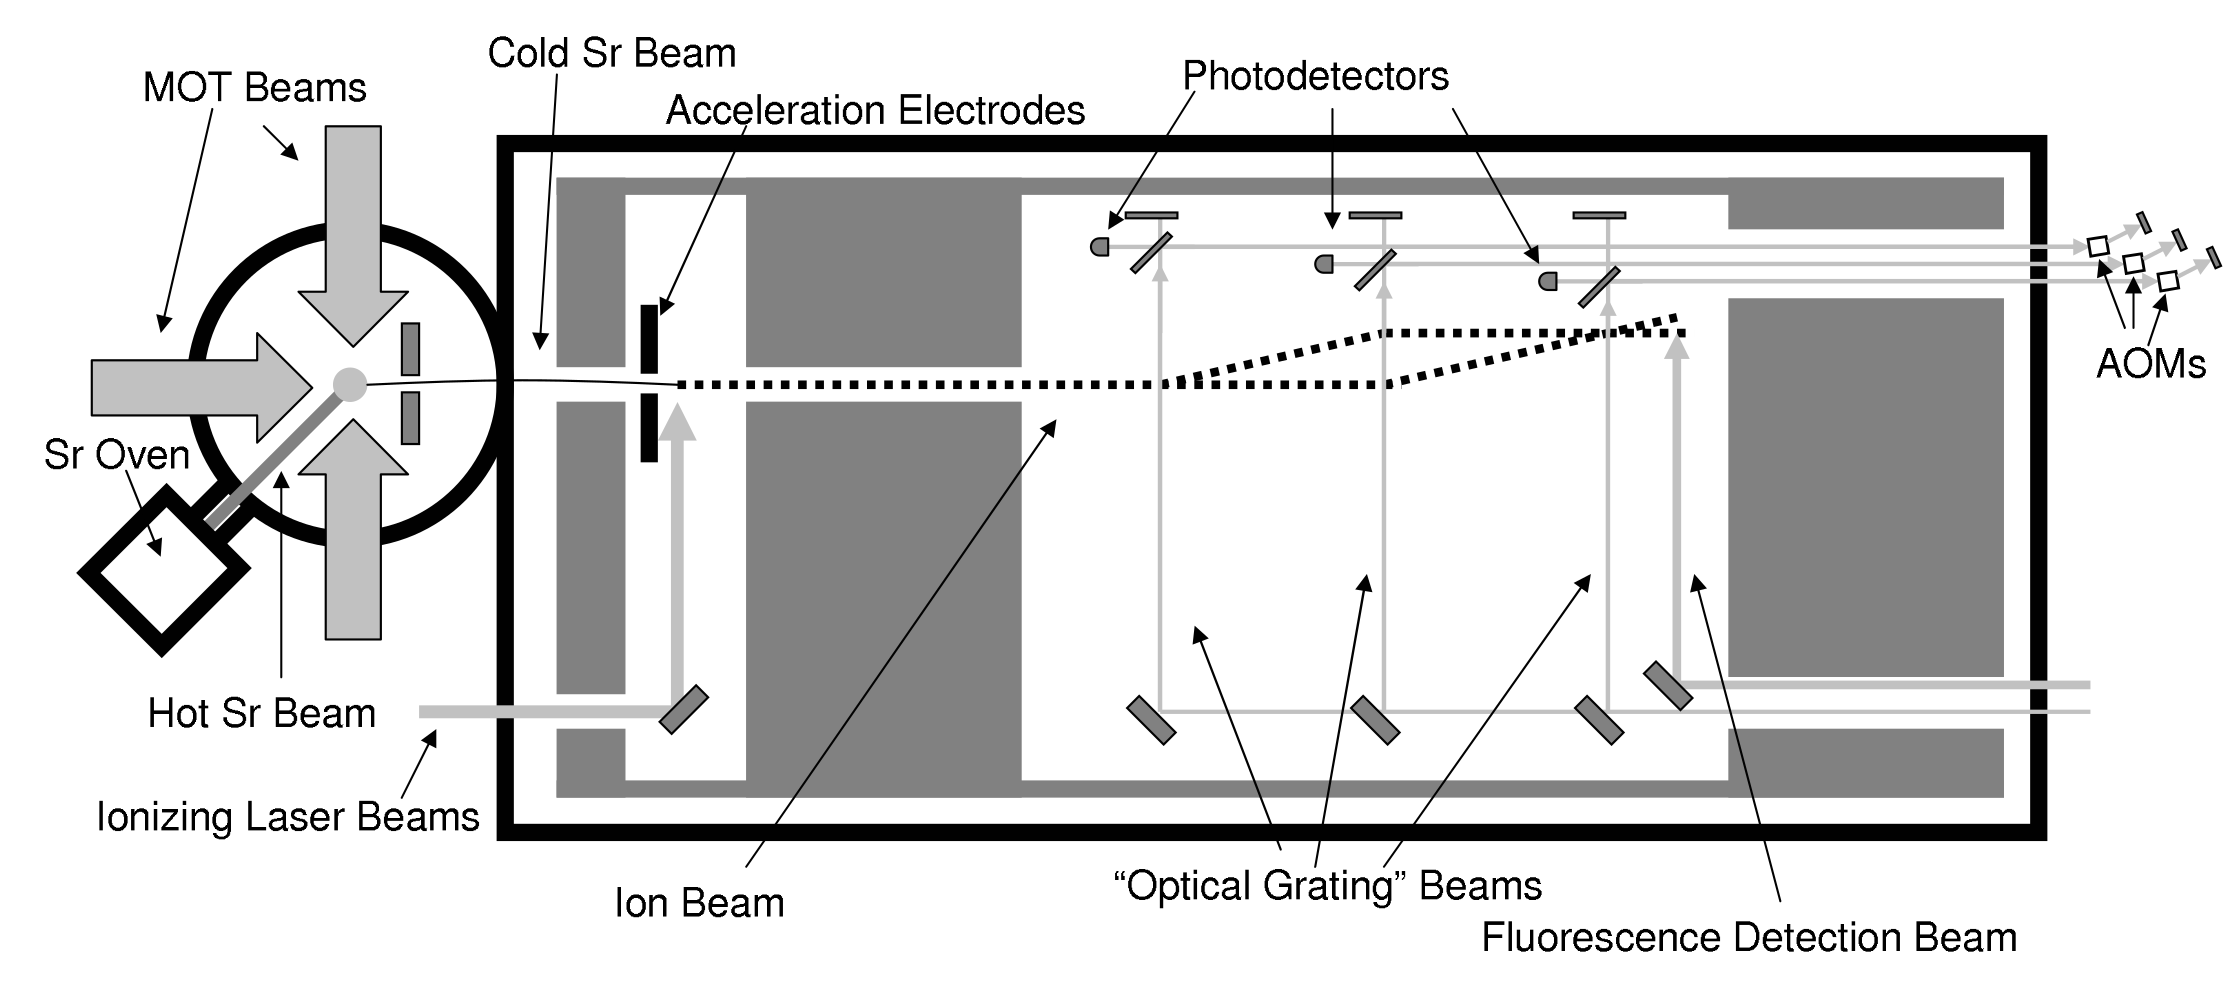
\includegraphics[totalheight=0.3\textheight]{interferometer_diagram}
}
\caption[Ion Interferometer]{\label{fig:IonInterferometer}
The entire Strontium interferometer. } 
\end{figure}

\section{Trapping of Neutral Strontium and Low Velocity Intense Source (LVIS)}

First, we must obtain a slow-moving beam of ionized $^{87}$Sr$+$. This is accomplished in two steps. 

We trap the $^{87}$Sr in a magneto-optical trap (MOT) using the standard techniques as outlined in Ref.\ \cite{cjeDiss}. 

The dominant cooling effect in the MOT is Doppler cooling. The trap consists of 6 red-detuned laser beams originating from the 460.8 nm laser system described in \cite{cjeDiss}. These point from each of six directions towards the center of the MOT. 

The 5s$^2$ $^1$S$_0$ to 5s5p $^1$P$_1$ transition is used to cool the atoms. This process selects the 87u isotope of Strontium \footnote{Further rejection of other Sr isotopes occurs because the Raman beams will not drive their transitions.}
The trapping is achieved using a pair of permanent rare-earth magnets. The Zeeman shift of the levels addressed by the the lasers traps them within a small range. The amount of trapped atoms is enhanced by our use of a Zeeman slower. 

We create an LVIS \cite{cjeDiss} following techniques developed by \cite{LVIS}. One of the mirrors in in the trap has a small hole drilled in it.\footnote{This hole was drilled in-house and the details of how we avoided damage and tests that verify the integrity of its optical surface can be seen in \cite{cjeDiss}} This allows some of the atoms to escape the trap. These atoms have a relatively narrow distribution of velocities. \footnote{Probably cite some other reference here--whoever invented/talked about the LVIS}

The atoms that drift out of the trap are then accelerated by a sort of Zeeman acceleration effect \footnote{i.e. the same as the effect exploited in a Zeeman slower, but they're not slowing down. The magnetic field gradients that cause this are created by the same magnets that are used to make the gradient in the middle of the trap.}

\section{Ionization of Strontium}
 
The next step is to selectively ionize the $^{87}$Sr to produce $^{87}$Sr$+$. This is accomplished using a pair of resonant transitions, which place the electron in a state in an autoionizing state whose energy is higher than the lowest energy states in the continuum. 

First, we stimulate the 5s$^2$ $^1$S$_0 \rightarrow$ 5s5p $^1$P$_1$ transition, which, conveniently, is the same 461 nm transition used to cool the atom. The second transition is the 5s5p $^1$P$_1\rightarrow$5p$^2$ $^1$D$_2$ transition. The $^1$D$_2$ state is 57 meV above the ionization threshold \cite{NSFprop}. This can be accomplished with a 408 nm laser. This can be achieved using GaN diode lasers \footnote{Maybe InGaN? It is the same diode laser technology used in Blu-ray players.}

\section{Acceleration of Beam}

The ions, which are at this point already travelling at some speed are then accelerated in an electric field produced by two pieces of copper held at constant potential. This gives us freedom to control the speed of the atoms. 


\section{Interferometry}

The interferometry is then achieved. 

%the waves that are interfered are the quantum mechanical matter waves of our atoms. I borrowed the words "atomic wave function" phrase from chu and kasevich

In order to produce two distinct paths, we uses stimulated Raman transitions as done by Ref.\ \cite{kasevichChu1991}. We use stimulated Raman transitions. This is a two photon process whereby we drive the atoms from one state to another using a third state as an intermediate state. We have 3 pairs of overlapping 408 nm lasers in our apparatus and each of these pairs is tuned to induce a stimulated Raman transition between the two $^2$S$_{1/2}$ ($5s$) ground states corresponding to $F=4$ and $F=5$. The transition uses the $^2$P$_{3/2}$ ($5p$) state as an intermediate state. 

%The stimulated Raman transition process is one whereby we 

The essential analysis will be saved for Chapter \ref{ChapterAboutTheAtoms}.


%trust yourself and know that you know it. and know that it doesn't have to be much better than it will be to be acceptable. 

%Is it true that at the end, we can distinguish between the F=4 and F=5 ground state of the Strontium? 
%I hope so. Those are the two states, haha. 





\chapter{Background}

\section{Basics of Ion Inteferometer}

This work includes an overview of ion interferometer experiment and a detailed exposition of the construction of the laser system that drives the stimulated Raman transitions.

The ion interferometer uses a Mach-Zehnder setup to achieve interferometry with $^{87}$Sr+ ions. 

Our 


\section{Historical Precedents}
In this section, we will discuss some related experiments as context for our experiment. This will include historical intellectual forebears and some more modern cousins. 
 \subsection{Interferometry with light}
Matter interferometry borrows many of its foundational concepts and terminology from interferometric light experiments. Though the interference of light has been the subject of serious study for a long time (e.g. Newton's rings), Young's double slit experiment is perhaps the quintessential optics experiment. Young placed two slits and passed light through them. He then observed a pattern of alternating dark and light fringes corresponding to the regions of constructive and destructive interference. 

The diffraction of light in this way is in fact directly analogous to the methods use in some matter-wave interferometry experiments. For example, Alex Kronin uses very small gratings to produce similar patterns \cite{Kronin_RMP}. 

DeBroglie hypothesized that matter exhibits wave-like behavior. Some of the earliest direct confirmation of this was achieved by Davisson and Germer, whose electron scattering experiment was directly analogous in interpretation to Bragg diffraction experiments performed using light. 

\subsection{Coherent Manipulation of Matter}
Matterwave interferometry arose with the development of techniques for the coherent control and measurement of atoms \cite{Kronin_RMP}. Rabi was among the first to use rf resonances to coherently control the internal states of molecules\footnote{I think this is right}. Ramsey's work in creating long-lived superpositions and the method of separate oscillatory fields was similarly seminal \cite{Kronin_RMP}. 
More recently, atom interferometers have been used for many different types of experiments. These have provided high-precision measurements of the fine structure constant \footnote{I'll have to find some citations. This is basically just a list of things I saw at conferences that I thought were cool}, investigations of gravitational effects and placed ever tighter limits on potential deviations from Standard Model physics. 
%\subsection{Charged Particle Atomic Physics}

\subsection{Laboratory-based electromagnetic tests}
One possible application of our apparatus is that it can be used to detect small electric fields in a setup like the one famously used by Cavendish in his early electrostatic experiments\footnote{I am not refering to the famous torsion balance gravitational experiment.} Cavendish effectively measured fundamental electrostatic constants by measuring the electric filed inside a charged, conducting enclosure. By demonstrating that the electric fields were 0 regarldless of the charge on the enclosure, Cavendish was able to deduce that the repulsion between like electric charges falls off in proportion to the inverse of the square of the distance between them. \footnote{todo: cite this guy later maybe:  http://geometrydude.wordpress.com/2012/12/22/cavendishs-phenomenological-derivation-of-coulombs-law/}. 


Our experiment is similar to Cavendish's experiment in two ways: First, our experiment will have a very similar setup as Cavendish's. The ion interferometer provides a sensitive way to measure electric fields inside a conducting shell that will be charged and discharged.  

The second way in which our experiment is related to Cavendish's is that it seeks to shed light on fundamental electromagnetic phenomena. Our our experiment seeks to measure fundamental electrical constants. Cavendish was able to measure the $1/r^2$ dependence in what eventually became known as Coulomb's law. Our experiment hopes to place a limit on the photon rest mass.\footnote{Our experiment will also produce results that may be reported as $\epsilon$ in the $1/r^{2+\epsilon}$ generalization of Coulomb's law.}
%footnote{who am I to say who did what first?}\cite{jackson} \footnote{it'd be nice to get Cavendish's original paper} 
%I don't really know if the finite conductivity of the shell matters for our experiment. 
%can we characterize copper in some way? I mean by taking time-dependent measurements of the dispersion of charge within the cavity? 
In fact, Cavendish's experiment directly inspired our experiment\footnote{This is a piece of lab oral history that I wanted to preserve}. Brian Neyenhuis, whose time working in Dallin's lab overlapped with mine, came across a practice GRE question about the best laboratory measurements to date confirming Coulomb's law. It turned out that these were a variation on Cavendish's method. They key limiting factor in all cases was the experimenter's ability to measure small electric fields inside the conducting shell. Brian started investigating the use of atomic physics techniques to improve these measurements. Soon he and Dallin had fleshed out their idea for creating an ion interferometer.  

According to Ref.\ \cite{jackson}. Many of the more recent tests of electrostatics were performed using setups similar to Cavendish's. 

%todo: find that paper that cites our experiment 
There are many other experiments along these lines as detailed in \cite{PhotonMassSurvey}. 

\subsection{More recent antecedent}
Electron interferometry using gratings has been achieved. \footnote{cite!!} Furthermore, ion interferometry has been achieved only using physical gratings. One of our experiment's main advantages is that its beamsplitters use no physical gratings

There are atomic clocks that use long-lived coherent superpositions of internal states of ions.\footnote{todo:cite}. However, The ions themselves do not enclose spacelike areas over the course of their path.

Coherent manipulation has also (thankfully!) been achieved in many labs \footnote{Todo:CITE!}. For example, neutral Sr has been trapped and cooled by XXXXX. 
Other experiments involving Sr TODO: add the other experiments.

The interest in $^{87}$Sr+ has been helpful not least because there are good numerical estimates of various transition parameters \cite{safronovaTheory}



\chapter{Laser System Overview}
%the sum of the whole is greater than the parts 

This chapter provides a broad introduction to the laser system addressed in this thesis. More information on the master laser configuration and setup can be found in Chapter \ref{generationOfSeedLight}. Information about the AOM configuration can be found in Chapter \ref{AOMInstallChapter}. The process of injection locking the slave lasers is discussed in more detail in Chapter \ref{InjectionLockingChapter}. Data from the working system can be found in Chapter \ref{triumphantDataChapter}.

This thesis describes the construction of the laser system (408 nm 5 GHz detuned laser system) that I built from 2010-2012. The purpose of this system is to produce two lasers which are near resonant with the 5s $^2$S$_{1/2}$ to 5p$^2$P$_{3/2}$ transition in $^{87}$Sr$+$, but which differ in frequency by precisely 5 GHz. This frequency corresponds to the hyperfine splitting of the ground state: the $F=4$ and $F=5$ ground states of $^{87}$Sr$^+$ differ in energy by $h 5GHz\approx 3.313 \times 10^{-24} J\approx 20.7 meV$. Tuning the lasers in this way is necessary to drive the stimulated Raman transitions for our ion interferometer project. 


\section{Basic Design}
%As we will find in Chapter\,\ref{ChapterAboutTheAtoms}, our ability to drive the transitions depends strongly on the difference between the lasing frequencies of our two lasers. In contrast, we expect our experiment to be relatively less sensitive to common mode drifts in the frequencies of our lasers.
The laser system consists of several components arranged together on a 12''$\times$48'' breadboard that is mounted to an optical table. The breadboard is enclosed by a plastic case. The current driver circuits and temperature controllers for the lasers are mounted on a shelf above the laser enclosure along with the RF generator, RF amplifier and various pieces of test and measurement equipment.  
\begin{figure}
    \centerline{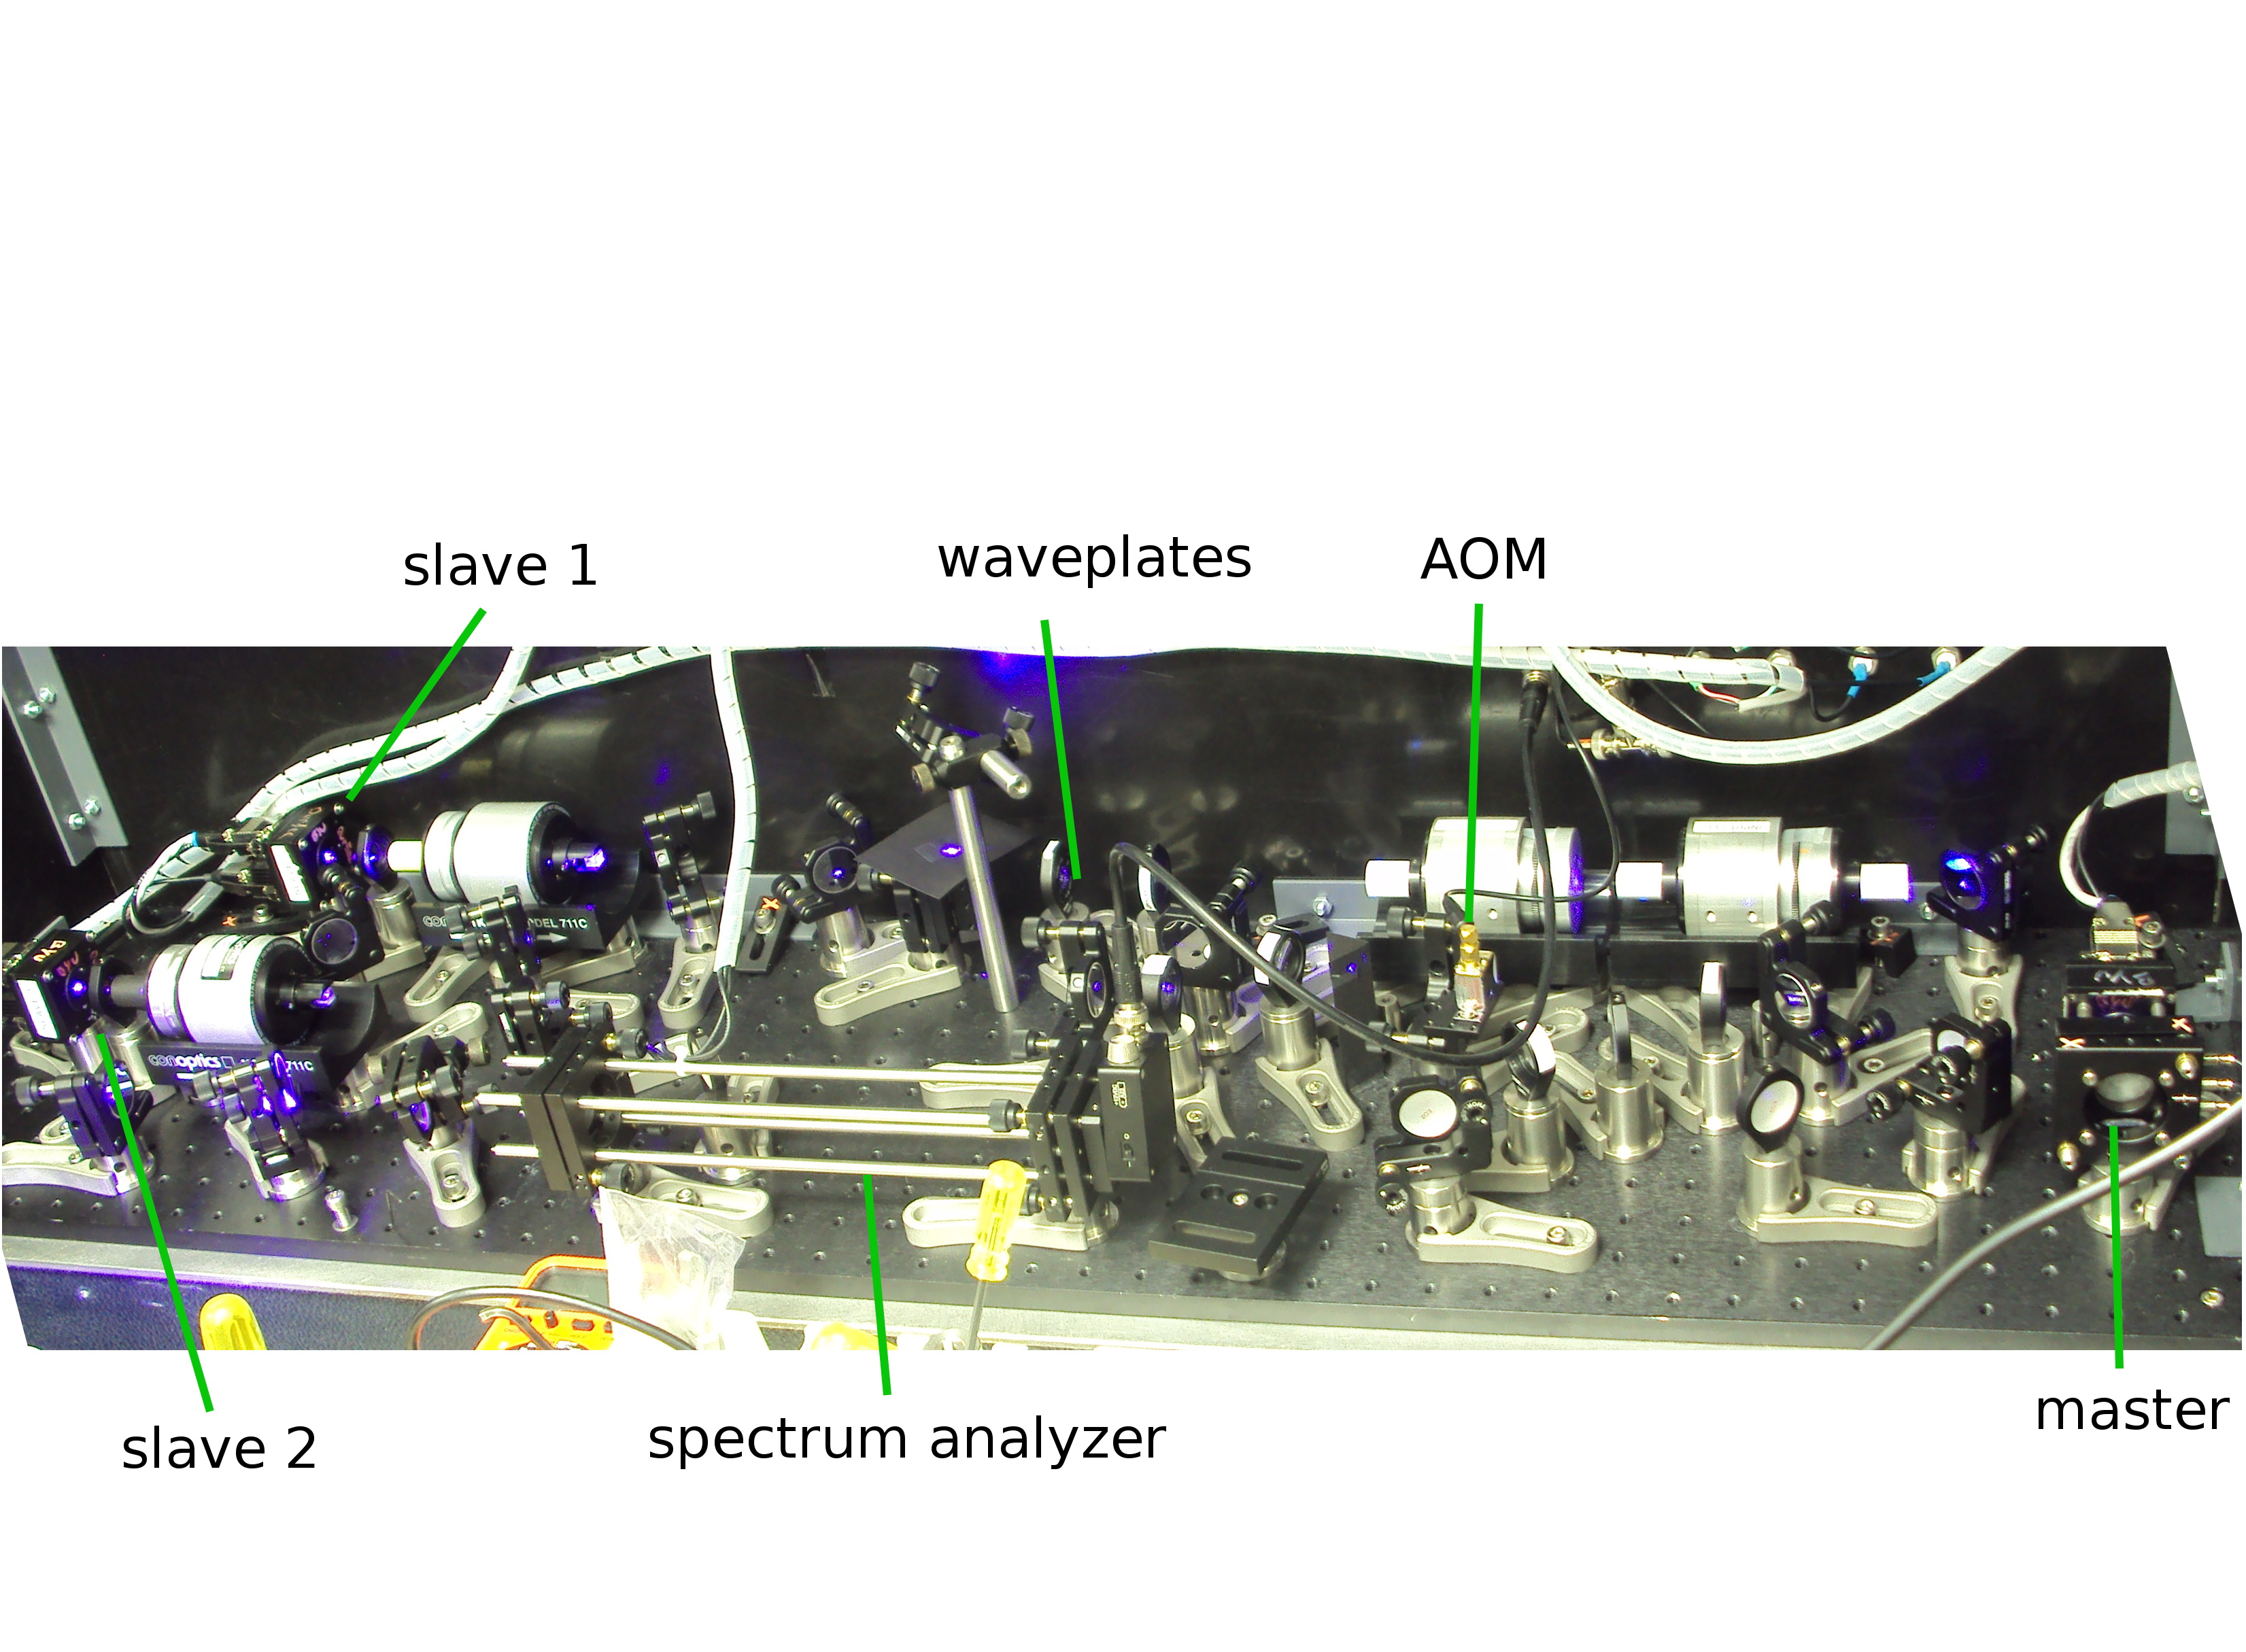
\includegraphics[width=1\textwidth]{entire_setup}}
    \caption[Photo of Entire System]{\label{fullexperimentphoto}
A photograph of the entire laser system while in operation. 
    }
\end{figure}

There are three separate laser diodes in housings. One of them is designated the ``master'' laser. The other two are designated ``slave 1'' and ``slave 2.'' The light that will actually be used on the atoms in the experiment is generated by the two slave lasers (slave 1 and slave 2).
 A diagram of the main components of the system can be found in Figure\,\ref{diagramOfSetup3} while a picture of the completed setup can be found in Figure\,\ref{fullexperimentphoto}. 

The system is designed so that some small fraction of the light coming from the master laser is shifted by an Acousto Optic Modulator (AOM) and used to seed the slave lasers. Coupling this light to the slave lasers and adjusting the slave lasers in such a way that they lase in a mode that is resonant with the shifted light coupled into them is what is meant by ``injection locking.'' 

The advantage of this setup is that as the frequency of the master laser drifts, both slaves will drift with it, while the relative frequency differnce between the slave lasers would remain stable.  As I will later show in Chapter \ref{ChapterAboutTheAtoms}, the experiment is less sensitive to common mode drift between the two slave lasers than it is to the drifting of the individual slaves relative to one another. 

%However, the difference in frequency between the slave lasers is set by an RF function generator with sub-Hz precision.

 %The master laser serves as a stable frequency reference so that the slave lasers can be seeded by it. 
Thus, the basic objectives that I accomplished were (1) to make a stable master laser tuned near the mean of the frequencies that we desire out of the slave lasers, (2) to shift the light from the master laser using an AOM (3) to couple the shifted light into the slave lasers and adjust the slave lasers so that they are able to oscillate in phase with the shifted light from the master laser.

\begin{figure}
    \centerline{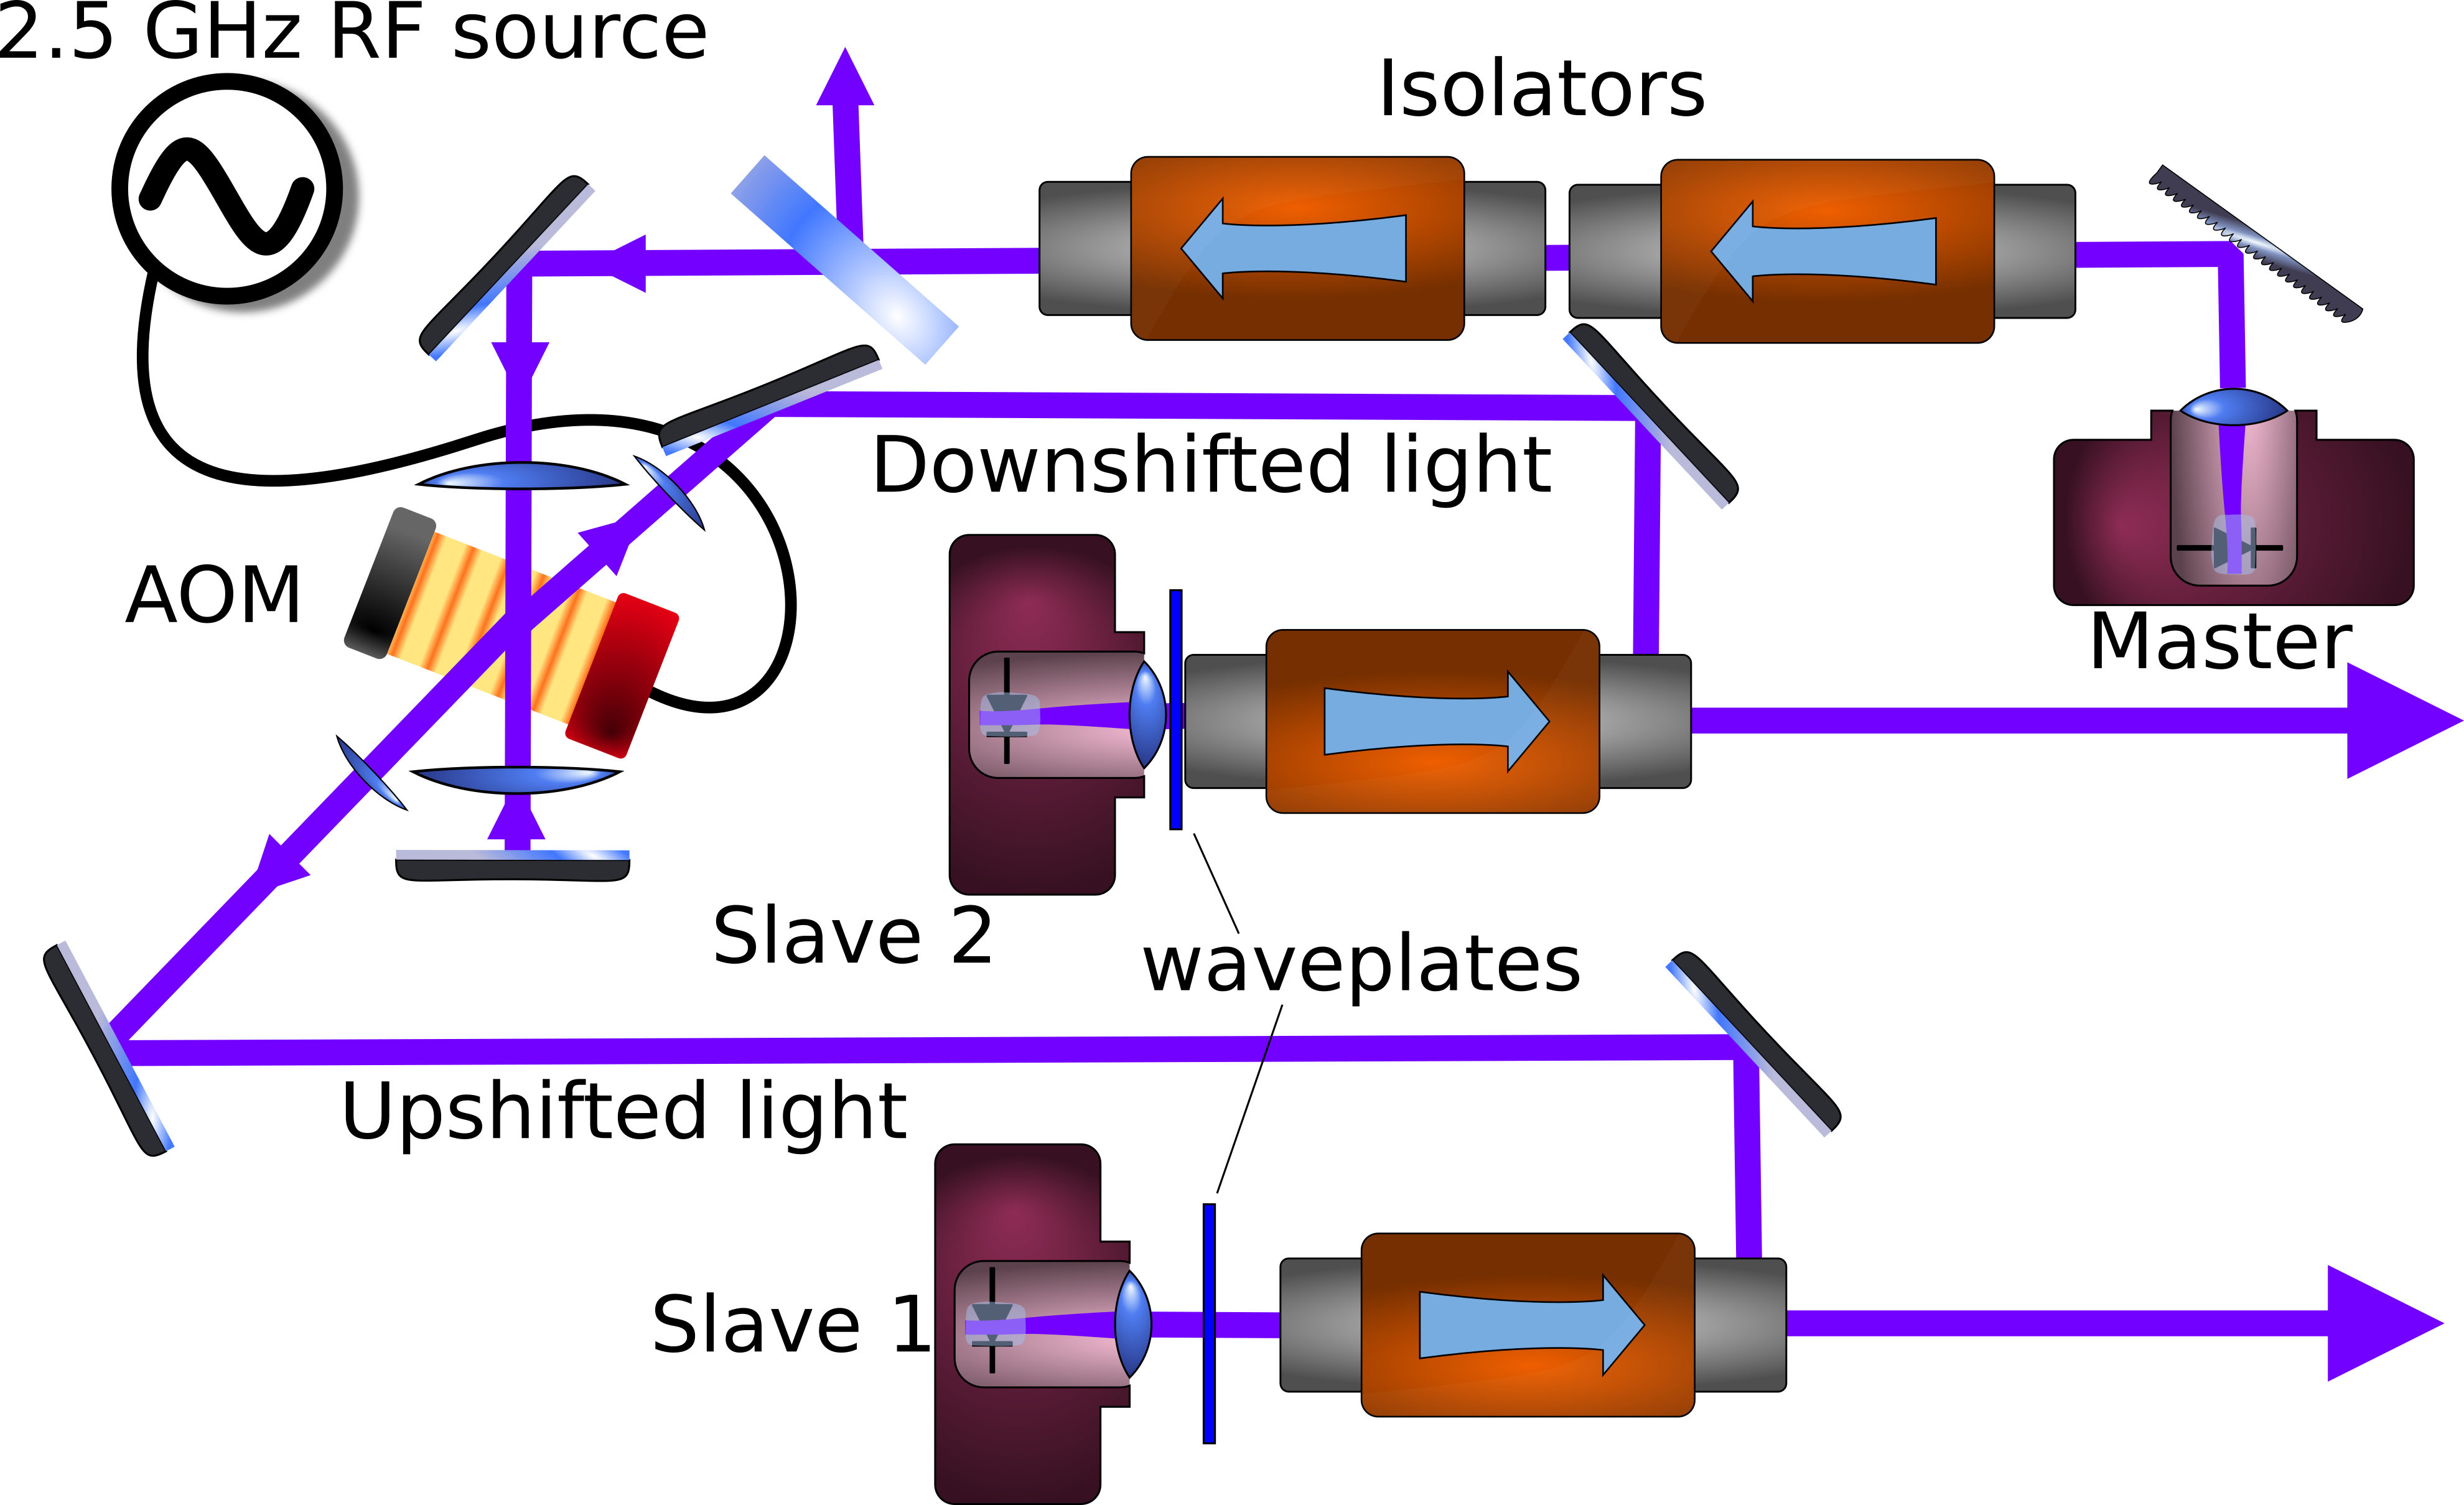
\includegraphics[width=1\textwidth]{diagramOfSetup3}}
    \caption[Diagram of the Setup]{\label{diagramOfSetup3}
	A schematic diagram of the basic pieces of the 408 nm 5 GHz detuned laser system apparatus. The master laser is depicted on the upper right. Its beam passes through two optical isolators in series. After this, the AOM is depicted with the upshifted and downshifted light coming out at exaggerated angles. These beams are then coupled into the rejection ports of two other optical isolators. Half waveplates are mounted in front of each of the slave lasers to rotate the polarization of the light to match the input polarizers on the isolators. The beams that will be used in the experiment are shown exiting through the lower right side of the diagram. The waveplates and polarizing beam cube that are used to adjust the light coupling into the AOM are not depicted.
    }
\end{figure}
\section{Following the beam path}
Light from the master laser passes through two optical isolators. These use Faraday rotation and a pair of glan polarizers to ensure that light travelling away from the master laser is allowed to propagate while light is prevented from coming back into the master laser. See Fig.~\ref{isolatorPicture}.

\begin{figure}
\centerline{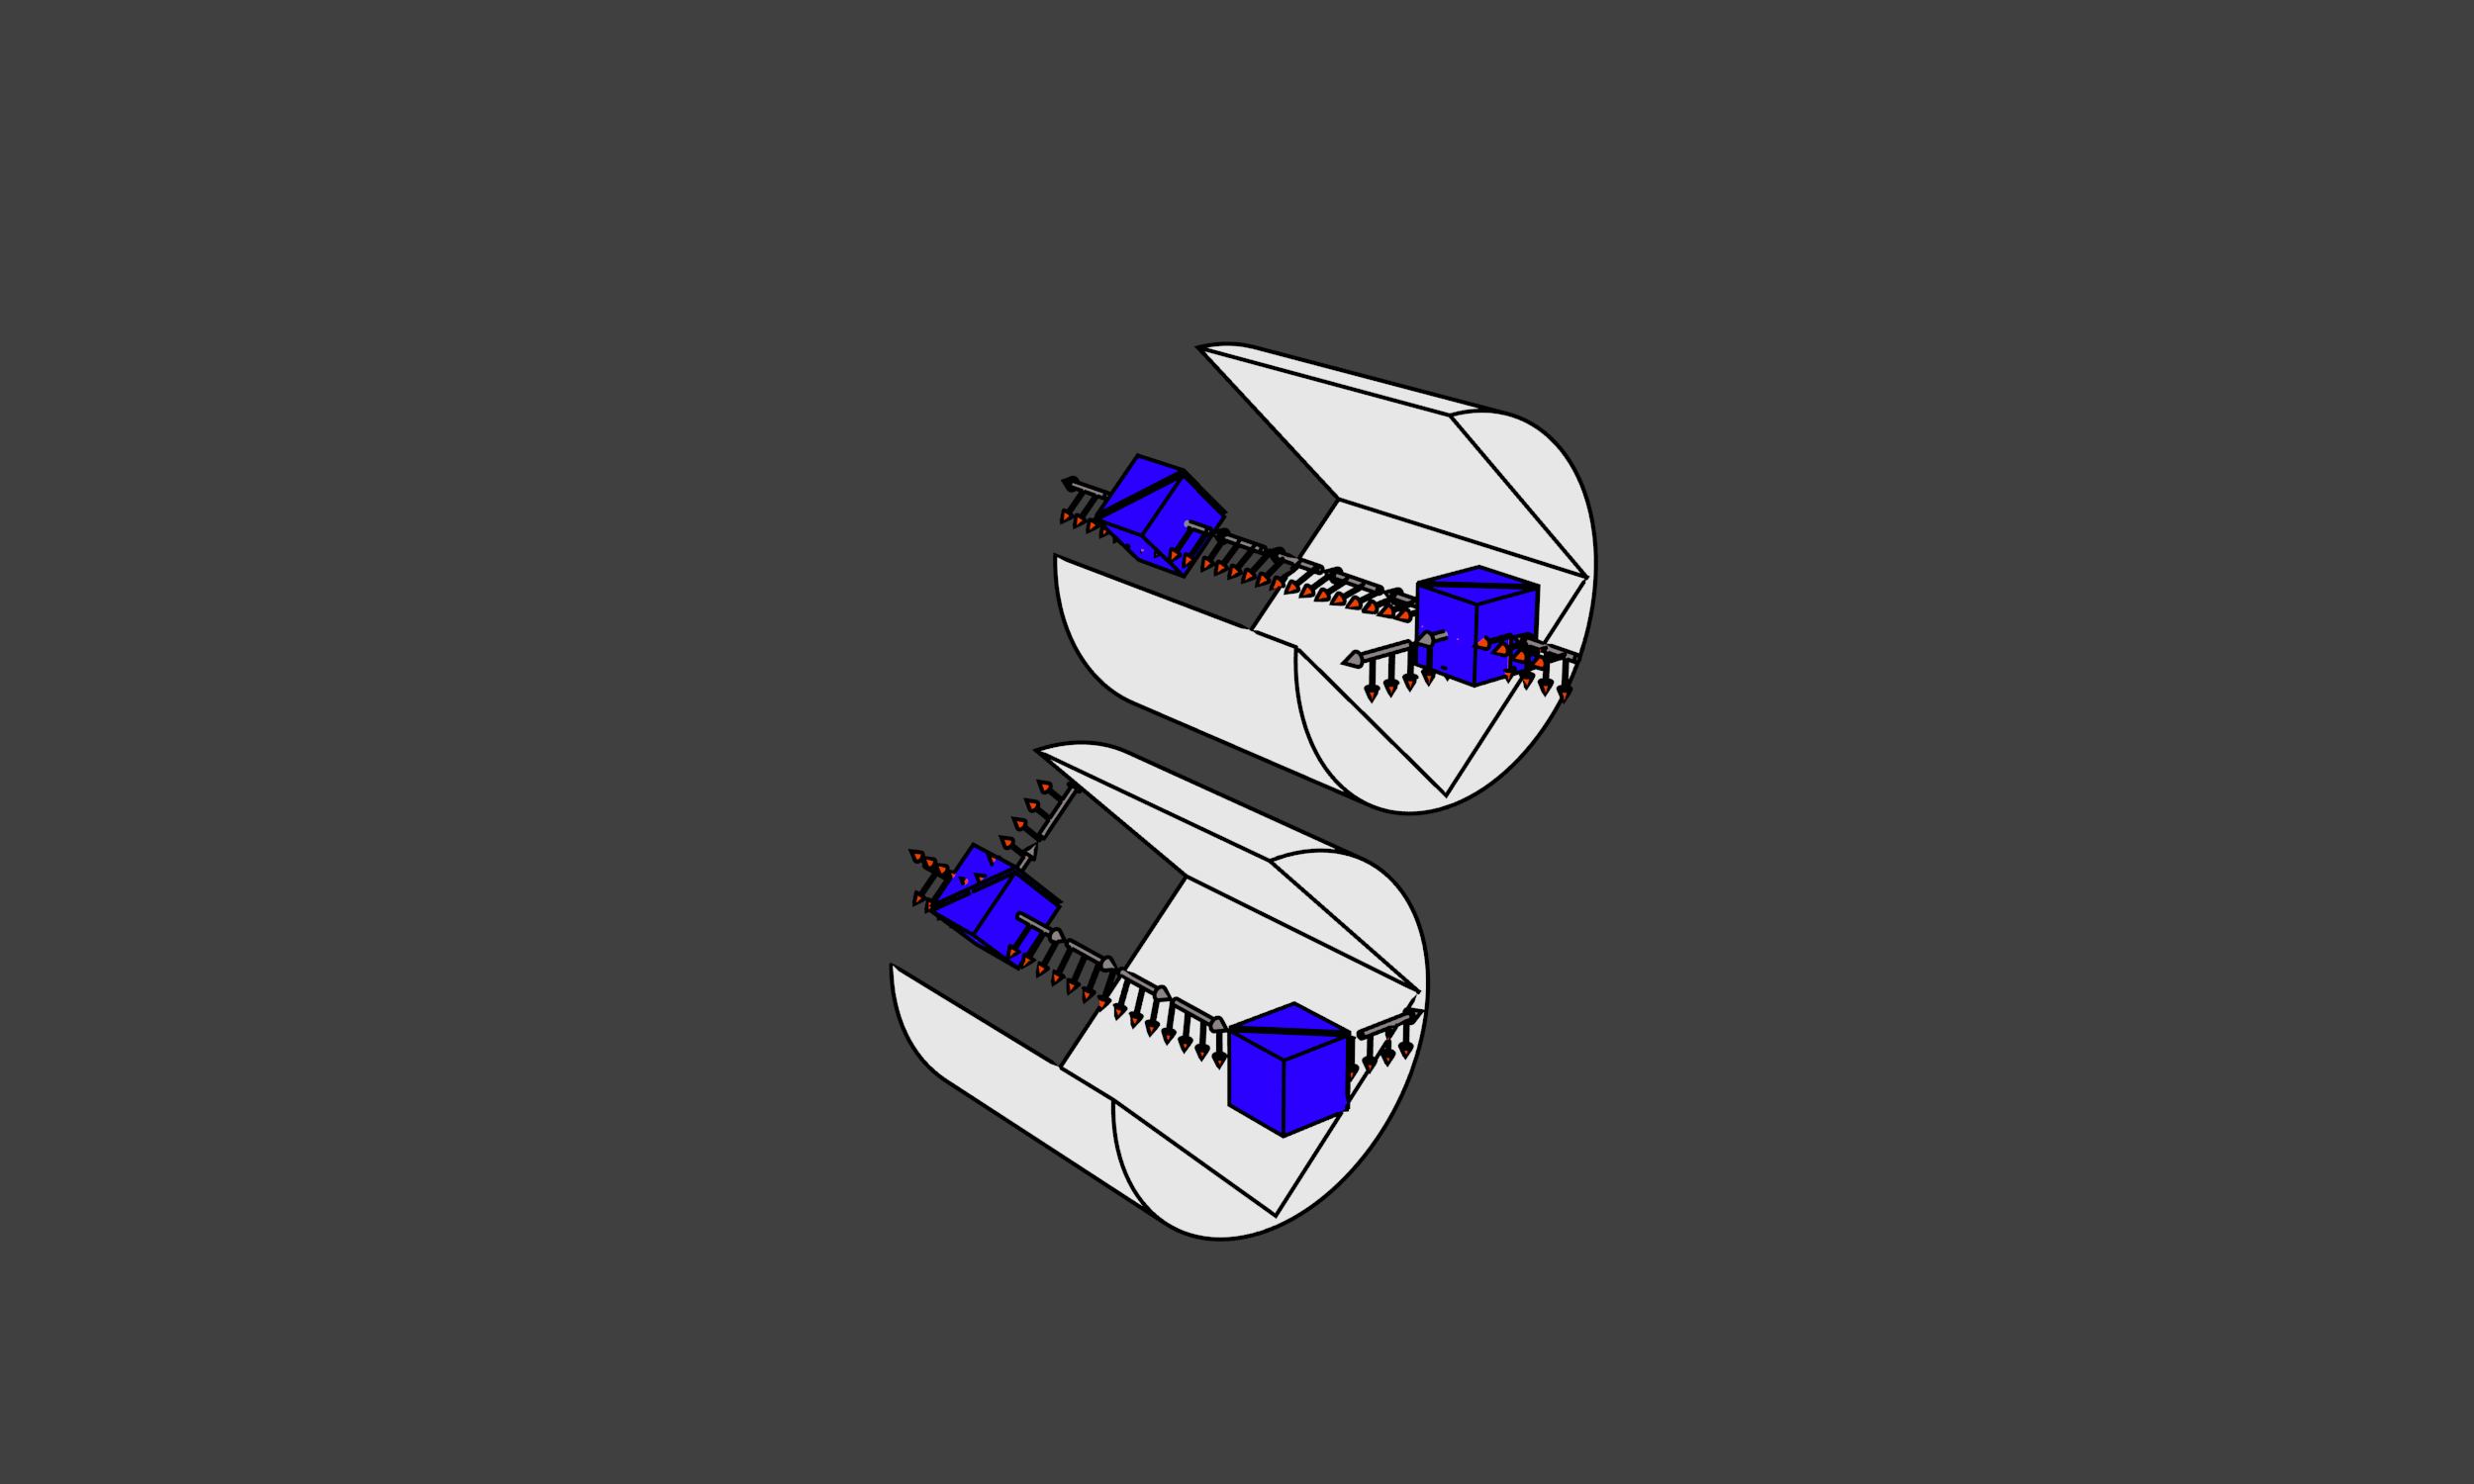
\includegraphics[width=1\textwidth]{isolators}}
\caption[Optical Isolator Illustration]{\label{isolatorPicture} Optical isolators work via Faraday rotation of the light. The Faraday effect occurs in certain materials when placed under a strong magnetic field. The Faraday effect results in the rotation of the polarization of light as it passes through a crystal. The direction of the change in polarization is depicted in the diagram. The image on the left shows an isolator rejecting light, while the image on the right depicts the same isolator allowing light travelling in the opposite direction to pass through.}
\end{figure}

Optical isolators are important because the stability of the master laser and the injection locking of the slave lasers requires control of the light being coupled into the laser cavity. By installing isolators, we can prevent unwanted reflections back into the master laser. This is an especially serious issue for the master laser since later in the beam path, we retroreflect the beam in such a way that, absent the isolators, light would couple directly back into the master laser. 

The beam then passes through a pair of waveplates and a polarizing beam cube, which serves the dual purpose of allowing us to attenuate the portion of the beam that goes through the AOM and splitting off a beam that can be used in our spectrum analyzer. A discussion of the method we used for adjusting the quantity of light passing through these waveplates can be found in Appendix \ref{twoWaveplateTrick}.

After this, the laser is passed twice through an Acousto-optic Modulator (AOM). The first-order diffracted beam from the first pass through the AOM produces light that is shifted up in frequency (down in wavelength). However, most of the power is contained in the 0th order beam that passes through the AOM without being shifted at all. We collimate this beam and retroreflect it, thereby sending it through the AOM in the opposite direction. This pass produces a weak beam that is downshifted in frequency. We thus end up with two beams, one of which is shifted upwards by 2.5 GHz and the other of which is shifted downward by 2.5 GHz. 

These two beams are then coupled into the two slave lasers. Each slave laser has an optical isolator in its beam path that allows light to travel out of the laser. Therefore, in order to couple light into the slave lasers, we have to use one of the rejection ports of the isolators. We couple light from 

The outputs of these two lasers are what we will use in our experiment to stimulate Raman transitions. Some of the light from each of the slaves are also redirected to the spectrum analyzer.

%We could have maybe used light coming out the rejection ports to monitor second order effects from the AOM. 

\begin{figure}
%    \centerline{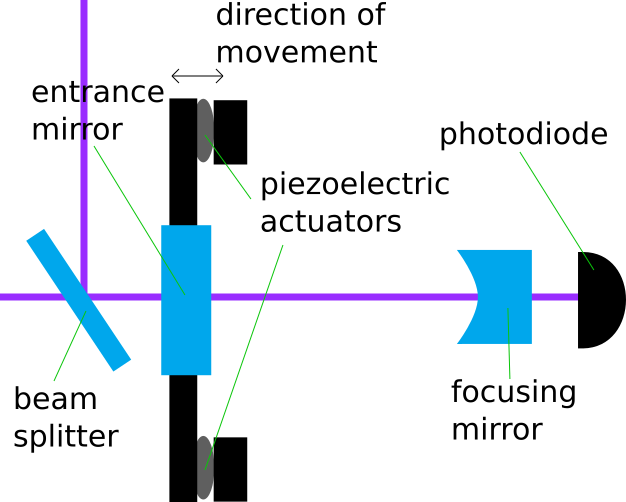
\includegraphics[trim=100pt 100pt 100pt 100pt, clip=true, totalheight=0.5\textheight,angle=90]{spectrumAnalyzer}}
    \centerline{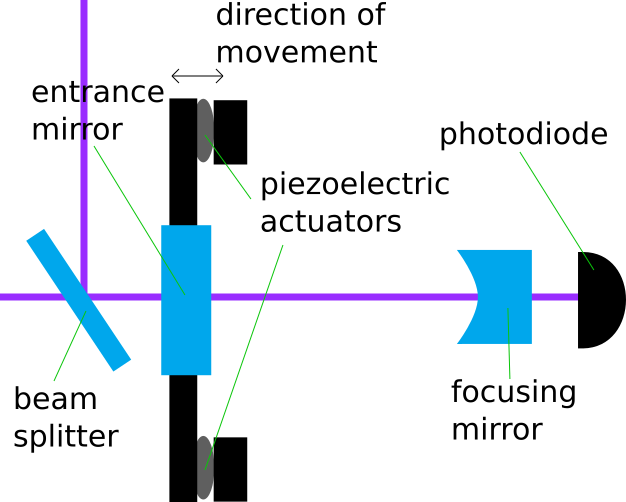
\includegraphics[totalheight=0.3\textheight ]{spectrumAnalyzer}}
    %\includegraphics[totalheight=0.3\textheight]{testfigure}
    \caption[]{\label{fig:spectrumAnalyzer}
    A diagram of the spectrum analyzer. The spectrum analyzer consists of a Fabry-Perot cavity of adjustable length. The photodiode on the far right of the diagram outputs a signal that shows when the incoming lasers are resonant. The left cavity mirror is mounted on a piezoelectric mount that allows us to finely displace the mirror using electronic controls. The master laser or either of the two slave lasers can be coupled to the cavity.
}
\end{figure} 

\section{Verifying that it worked}
We use a Fabry-Perot spectrum analyzer to monitor whether the slaves are injection locked and to verify that the master laser and slave lasers are running single mode. The spectrum analyzer is depicted in Fig.\,\ref{fig:spectrumAnalyzer}. 
The spectrum analyzer is a semiconfocal cavity of length 200 mm. The flat, partially reflective mirror through which light enters the cavity is mounted on a mount that features piezo-electric actuators. At the other end is a curved mirror of focal length 200 mm. Behind this is a photodiode \footnote{the Thorlabs DET family of reversed biased photodiode products}.

The length of the optical cavity in the spectrum analyzer is thus modulated by sweeping the voltage that we put across the piezoelectric crystals. When the cavity length is such that the coupled light is close to a resonance of the cavity, we expect to see higher signal on the photodiode. 
The piezoelectric actuators are connected to a commercially available piezo control box that sweeps the voltage in a sawtooth wave type pattern, with a frequency $\sim$20Hz. 

The free spectral range of the spectrum analyzer describes exactly how far apart we expect the peaks to be. In the case of a hemiconfocal cavity like ours, the free spectral range is given by 

\begin{equation}
    \textnormal{FSR}=\frac{c}{8L}
\end{equation}

Therefore, we expect that as we scan the input mirror, we will see the same peaks coming into and out of resonance. The period over which this pattern repeats corresponds to scanning 187 MHz. Thus, if we have two peaks on the spectrum analyzer, we should be able to glean some information about how far apart they are.

A more complete discussion of the spectrum analyzer can be found in Appendix \ref{spectrumAnalyzer}.

\chapter{The Atoms} \label{ChapterAboutTheAtoms}
\section{Overview of relevant atomic transitions}

Our objective in this chapter is to calculate the necessary intensity and beam waist that will allow our lasers to impart the $\pi$ and $\pi/2$ pulses to the atoms as they make their way through the chamber. In order to show why we believe our laser can provide the $\pi$ and $\pi/2$ pulses, we must first take a detailed look at the Raman transitions we are trying to drive. 

Thus, the purpose of this chapter is threefold:
\begin{itemize}
\item Identify the relevant states of our atoms.
\item Find and interpret appropriate numerical values for relevant parameters in our Hamiltonian.
\item Model the dynamics of the atom.
\item Calculate the appropriate intensity, width and polarization of our laser beams that will allow us to impart the $\pi$ and $\pi/2$ pulses to the atom. 
\end{itemize}

\begin{figure}
\centerline{
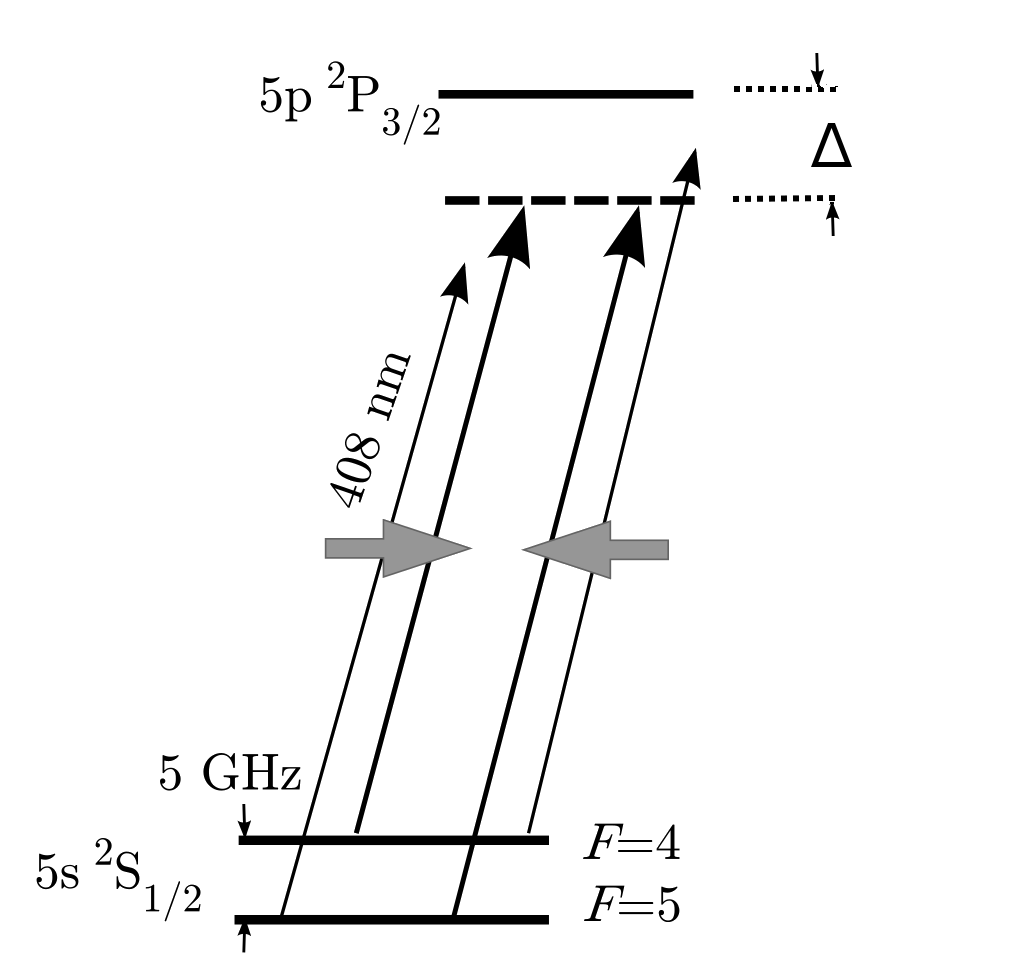
\includegraphics[totalheight=0.3\textheight]{E_level_from_proposal}
}
\caption[Energy Level Diagram for $^{87}$Sr+]{Energy Level Diagram for $^{87}$Sr+. The hyperfine ground states are separated by a small energy. Diagram is not to scale: a scaled diagram would show the splitting between the $F=4$ and $F=5$ states to be about 147,000 times smaller than the splitting between the $^2$S$_{1/2}$ states and the $^2$P$_{3/2}$ states.}
\end{figure}

%In Ref.\ \cite{cjeDiss}, this calculation is performed, but some of the details are left mysterious. In particular, no source is cited for any of the physical parameters of the $^{87}$Sr+ atom (e.g. the dipole moment values, the transition width, the saturation parameter). We hope to reproduce this calculation with more details.  

\section{States and Quantum Numbers}

The Hamiltonian of the Strontium ions is analagous to the Hamiltonian of a single-electron atom. 
In a single electron atom, the solution to the Schr\"odinger equation describing the electron is solved by separation of variables.
 Each solution is a product of a spherically symmetric function that depends only on the distance $r$ from the nucleus and the spherical harmonics.
This is because the orbital angular momentum operator $\mathbf{L}$ commutes with such a Hamiltonian. In fact, the orbital angular momentum operator commutes with any Hamiltonian with a spherically symmetric potential.
Thus, we can use the familiar angular momentum quantum numbers for the eigenstates of any spherically symmetrical Hamiltonian.

In the case of $^{87}$Sr+, there is only one electron in the valence band. The inner shells are full and we assume that the symmetry is such that the eigenstates of the atom will also be eigenstates of the orbital angular momentum operator, $\mathbf{L}$.
 The system also involves two other angular momentum operators: the spin operator for the valence electron, $\mathbf{S}$%\footnote{The spin of the electrons on the inner shells cancels and adds to 0} 
and the spin of the nucleus $\mathbf{I}$ \footnote{Here and throughout, we will use the boldface $\mathbf{I}$ to mean the operator while the unbolded letter ($I$) will mean the associated eigenvalue.}.
%We will first approximate the Hamiltonian by assuming that there is no coupling that is dependent on the spin. 
%The hyperfine interaction will be modeled as a perturbation on top of this.

The ``good'' quantum numbers for describing the internal states of a $^{87}$Sr+ ion are $F$,$J$,$L$,$S$,$m_f$ and $n$\cite{experimental_hyperfine_alkali_arimondo}\cite{cuaMITnotes} where $F$,$J$,$L$,$S$,$m_f$ take on their usual meanings (see Table\,\ref{quantumNumberQuickref}). This is because the Hamiltonian is diagonal in this basis.

\begin{table}[h!]
\centering
\begin{tabular}{|c|l|}
\hline
Quantum Number & Definition and comment \\ \hline \hline
L & Orbital angular momentum of valence electron. \\ \hline
S & Spin of valence electron. Takes on values $\pm 1/2$ \\ \hline
I & Nuclear spin. For $^{87}$Sr$^+$, $I=9/2$ \\ \hline
J & Total valence electron angular momentum. $\mathbf{J}=\mathbf{L}+\mathbf{S}$ \\ \hline
F & Total angular momentum $\mathbf{F}=\mathbf{I}+\mathbf{J}$ \\ \hline
$m_f$ & Eigenvalue of $\mathbf{F}_z$.\\ \hline
\end{tabular}
\caption{The quantum numbers used to describe the internal state of the $^{87}$Sr+ ion. These are conventional choices; the table is provided only for convenience.}
\label{quantumNumberQuickref}
\end{table}

%why does the ground state J not play into it at all?
%I just realized I have no idea where to find the information on the hyperfine splitting of the Sr+ 
%also, IDK what to do about the the Nuclear spin numbers of the upper state. 
%I have this http://link.springer.com/article/10.1007%2FBF00568145

Our experiment is designed to use the $^2$S$_{1/2}$ and $^2$P$_{3/2}$ states. Each of these spectroscopic terms refers to many states: First, we must account for the states that correspond to different values of $F$. Since $\mathbf{F}=\mathbf{I}+\mathbf{J}$, $F$ can take on any values between $|I-J|,|I-J+1|,...,|I+J|$. So, for example, since $I=9/2$, the valid values of $F$ for the $^2$S$_{1/2}$ state are $F=4$ and $F=5$. For the upper states, where $J=3/2$, $F$ can take on the values $3,4,5,6$ 

%there are some dipole transition selection rules governing $F$ \cite{sobelman_spectra}:
%\begin{align}
%&\Delta F=0,\pm 1\\
%&F+F'\geq 1
%\label{FselectionRules}
%\end{align}
%This allows us to immediately restrict our discussion of the $^2$P$_{3/2}$ states to only include the ones with $F=3,4,5,6$. We have 
%
%Now, the selection rules can be determined by the operation of the C-G coefficients. 

%\begin{table}[h]
%\centering
%\begin{tabular}{|l|l|||r|}
%\hline
%$F=4$ $^2$S$_{1/2} (5s)$ & Ground state  \\ \hline
%$F=5$ $^2$S$_{1/2} (5s)$ & Ground state  \\ \hline
%$F=3$ $^2$P$_{3/2} (5p)$ & Intermediate state  \\ \hline
%$F=4$ $^2$P$_{3/2} (5p)$ & Intermediate state  \\ \hline
%$F=5$ $^2$P$_{3/2} (5p)$ & Intermediate state  \\ \hline
%$F=6$ $^2$P$_{3/2} (5p)$ & Intermediate state  \\ \hline
%\end{tabular}
%\caption{Relevant states}
%\label{tableOfStates}
%\end{table}

\section{Review of Hyperfine Splitting}

We now discuss the Hyperfine contribution to our overall Hamiltonian. We will need to understand the hyperfine splitting to allow us to model the 5GHz energy difference between the $F=4$ and $F=5$ $^2$S$_{1/2}$ states. Our discussion will allow us to calculate hyperfine shifts for all the energy levels in our atom based on the hyperfine $A$ and $B$ coefficients, for which we have found experimental and numerical estimates in the literature.

\subsection{Hyperfine basics}

The hyperfine splitting arises from interactions between the nucleus and the electrons. In general, we can split out the Hamiltonian of the Hyperfine interaction as follows: 

\begin{equation}
H=H_0+H_{\mathrm{hfs}}
\end{equation}

where $H$ represents the total Hamiltonian of the system, $H_0$ represents the Hamiltonian neglecting the hyperfine interaction and $H_{\mathrm{hfs}}$ represents the piece of the Hamiltonian that models the hyperfine interaction. 

The standard expansion of $H_{\mathrm{hfs}}$ in the literature is:  

\begin{equation}
H_{\mathrm{hfs}}=\sum_k \mathbf{T}^{(k)} \cdot \mathbf{M}^{(k)} \label{hfs_hamiltonian_eqn}
\end{equation}
\cite{schwartz_hyperfine_expansion}
\cite{experimental_hyperfine_alkali_arimondo}
\cite{chinesePhysics}
%\footnote{todo: cite that review article and the lecture notes you found}

where $\mathbf{T}^{(k)}$ and $\mathbf{M}^{(k)}$ are irreducible spherical tensor operators of rank $k$.
\footnote{Recall that the dot product for spherical tensors of arbitrary rank is defined as follows:
\begin{equation}\label{TkMk_hyperfine}
\mathbf{T}^{(k)}\cdot\mathbf{M}^{(k)}=\sum (-1)^qT_q^{(k)}M_{-q}^{(k)}
\end{equation}
}
 $\mathbf{T}^{(k)}$ represents information about the electron.
$\mathbf{M}^{(k)}$ represents the nucleus.\cite{experimental_hyperfine_alkali_arimondo}\cite{schwartz_hyperfine_expansion}
\cite{sobelman_spectra}
Writing the expansion in this form shows explicitly the geometry of the operator. 

Before discussing what information $\mathbf{T}^{(k)}$ and $\mathbf{M}^{(k)}$ represent exactly,
we pause to point out a few geometrical facts. Even if we had no knowledge of the mechanism by which hyperfine interactions occur, we might still arrive at Eq.\,\ref{hfs_hamiltonian_eqn} simply by geometrical considerations.
Notice that the generator of rotations under which $\mathbf{T}^{(k)}$ is valid is the electron total angular momentum, $\mathbf{J}$, while $\mathbf{M}^{(k)}$ is subject to rotations defined in terms of the nuclear angular momentum operator $\mathbf{I}$. 
The direct product of these two gives us a value that can be validly rotated using the group generated by the combined angular momentum operator $\mathbf{F}$.\cite{Racah2}\cite{sobelman_spectra}. Thus, each term of our expansion has two parts: one that is a valid tensor operator associated with the geometry of the nucleus and one that is a valid tensor operator associated with the geometry of the electron. By combining these two parts using a dot product, we see that each term turns out to be a valid tensor operator for the entire atomic system. This is exactly what we would expect.

The most important contributions to the Hyperfine splitting come from magnetic dipole interactions and electric quadrupole interactions \cite{sobelman_spectra}\cite{schwartz_hyperfine_expansion}\cite{cuaMITnotes}. These correspond to the $k=1$ and $k=2$ terms in Eq.\,\ref{TkMk_hyperfine} respectively\cite{experimental_hyperfine_alkali_arimondo}.
%\footnote{It is interesting to note that the odd values of $k$ correspond to magnetic interactions while the even values correspond to electric interactions. That is to say that there is no electric dipole interaction between the electrons and the nucleus, but there is a magnetic dipole ($k=1$), while there is an electric quadrupole coupling, but no magnetic quadrupole, etc}
\subsection{Magnetic Dipole Interaction}

First, we discuss the $k=1$ term, or magnetic dipole interaction term from the expansion in Eq.\,\ref{TkMk_hyperfine}. Classically, we know that the potential energy of a dipole in a magnetic field is proportional to the dot product of the magnetic dipole moment vector with the magnetic field vector ($U=-\mathbf{\mu}\cdot\mathbf{B}$). We also know that the magnetic field at the center of a classical dipole points in the direction of the dipole moment. Therefore, it seems reasonable that the energy due to the interaction of the electron and the nucleus might be somehow proportional to a dot product of two vectors representing their respective angular momenta. Indeed, this turns out to be the case: the magnetic dipole interaction can be written as follows\cite{sobelman_spectra}: 
\begin{equation}\label{IdotJ}
W_f=A\mathbf{I}\cdot\mathbf{J}
\end{equation}
where $W_f$ represents the energy associated with this coupling and $A$ encapsulates a coupling factor between the nuclear and electronic magnetic moments. 
%Note that here we are using the normal, three dimensional dot product (i.e. $\mathbf{I}\cdot\mathbf{J}=I_xJ_x+I_yJ_y+I_zJ_z$). 

The product $\mathbf{I}\cdot\mathbf{J}$ can be expanded by noticing that $\mathbf{F}^2=(\mathbf{I}+\mathbf{J})^2=\mathbf{I}^2+2 \mathbf{I}\cdot\mathbf{J}+\mathbf{J}^2$. This gives \cite{cuaMITnotes}\cite{sobelman_spectra}: 

\begin{equation}\label{Wf_dot_product}
W_f=\frac{1}{2}A(\mathbf{F}^2-\mathbf{J}^2-\mathbf{I}^2)
\end{equation}

We can also see how Eq.\,\ref{IdotJ} represents the $k=1$ term in Eq.\,\ref{TkMk_hyperfine}. We clearly have one tensor operator from the Nuclear angular momentum space ($\mathbf{I}$) along with one vector from the electron angular momentum space ($\mathbf{J}$). The product we get is a scalar that will be invariant under rotations in the total space\footnote{A quick note about constants. In the expansion in Eq.\,\ref{TkMk_hyperfine}, there are different conventions \cite{schwartz_hyperfine_expansion} for deciding which coefficients are pulled into which operators. However, as we will see, the coefficient $A$ as used in Eq.\,\ref{IdotJ} is defined in a standard way and can be looked up in the literature. For this reason, we are specifying $T$ and $M$ only up to a constant. This is fine since the point of showing the expansion is really just to make a comment about the geometry of hyperfine interactions, while the actual calculations only involve the first two terms}.

\subsection{Electric Quadrupole Interaction}
In a similar way, the $k=2$ term in Eq.\,\label{TkMk_hyperfine} can be shown to correspond to the electric quadrupole interaction. Chapter 6.2 of Ref.\,\cite{sobelman_spectra} gives a good explanation for this. The crux of the argument is that the electric quadrupole interaction,
\begin{equation}
W=\int\frac{\rho(\mathbf{r})\rho'(\mathbf{r}')}{|\mathbf{r}-\mathbf{r}'|}d\mathbf{r}d\mathbf{r'}\\
\end{equation}
can  be expanded in terms of spherical harmonics: 
\begin{equation}
W=\int d\mathbf{r}d\mathbf{r'}
\rho(\mathbf{r})\rho'(\mathbf{r}')\sum_k \frac{r'^k}{r^{k+1}}[C^k(\theta,\phi)\cdot C^k(\theta',\phi')] \label{quadrupole_expanded}
\end{equation}

The $k=2$ term in the integral contained in Eq.\,\ref{quadrupole_expanded} takes the form of an inner product between two rank 2 spherical tensors. Thus, we are satisfied that we have found the $k=2$ terms in Eq.\,\cite{TkMk_hyperfine}.

The inner product between two rank 2 spherical tensors can be evaluated using Eq. 4.169 from Sobelman \cite{sobelman_spectra} (the formula can also be found in Ref.\,\cite{Racah2} and is also referred to in Ref.\,\cite{schwartz_hyperfine_expansion}):

\begin{multline}\label{4169_combine_diff_tensors}
\langle\gamma I J F M_f|(T^{(k)}M^{(k)})|\gamma J I F M_f\rangle \\
=
(-1)^{F+I+J} \sum_{\gamma} \langle\gamma J||T^{(k)}||\gamma J\rangle
\langle\gamma I || M^{(k)} ||\gamma I\rangle
\begin{Bmatrix}
J & I & F \\
I & J & k
\end{Bmatrix}
\end{multline}
where 
$\begin{Bmatrix}
J & I & F \\
I & J & k
\end{Bmatrix}$ represents the Wigner $6j$ symbol. 

Using the properties of the Wigner $6j$ symbols, it can be shown that \cite{cuaMITnotes}\cite{sobelman_spectra}, 

%\footnote{I will get this from Sobelman. He gives the Racah coefficients in 4.97 - 4.99} 
the equation for the electric quadrupole term in the hyperfine interaction takes the form:
%\footnote{OK Dallin--I'm not sure if I should even include this.} 

\begin{equation}\label{justQuadrupole}
W=BC(C+1)
\end{equation}
where 
\begin{equation}
C=[F(F+1)-J(J+1)-I(I+1)]
\end{equation}

(Interestingly, Eq.\,\ref{Wf_dot_product} can also be evaluated using Eq.\,\ref{4169_combine_diff_tensors} using $k=1$.)

\subsection{Write both hyperfine terms in terms of standard constants}
We can rewrite Eq.\,\ref{dot_product} in terms of $C$ 
and then combine it with Eq.\,\ref{justQuadrupole} to get the full hyperfine splitting\cite{cuaMITnotes}: 

\begin{equation}\label{Standard_hyperfine_AB}
E_{\mathrm{hfs}}=\frac{1}{2}AC+BC(C+1)
\end{equation}

The coefficients $A$ and $B$ as used in Eqs.\,\ref{Standard_hyperfine_AB} and \ref{Wf_dot_product} are the hyperfine A and B coefficients. $A$ and $B$ are a standard name and notation used in calculating hyperfine energy shifts. Their values can be looked up in the literature\cite{cuaMITnotes}.  We found values for the $A$ and $B$ coefficients for $^{87}$Sr+ in Ref.\,\cite{safronova2photon}. These are summarized in Table\,\ref{AB_table}\footnote{These are \emph{not} the Einstein $A$ and $B$ coefficients relating to radiative transition rate. Though, unfortunately, we will have to mention the Einstein $A$ and $B$ coefficients later.}.  

\begin{table}[h]
\centering
\begin{tabular}{|l|r|r|r|}
\hline
Level &  $A^{\mathrm{(SDpT)}}$ &$A^{\mathrm{(theor)}}$ & $A^{\mathrm{(expt)}}$ \\ \hline \hline
$5s ^2$S$_{1/2}$&-997.85 MHz& -1000 MHz& -1000.473673(11) MHz\\ \hline
$5p ^2$P$_{3/2}$&-35.26 MHz&-35.3 MHz&-36.0(04) MHz\\ \hline
\end{tabular}

\begin{tabular}{l}
%This is just for spacing it
%\quad \\
\end{tabular}

\begin{tabular}{|l|r|r|r|}
\hline
Level &  $B^{\mathrm{(SDpT)}}$ &$B^{\mathrm{(theor)}}$ & $B^{\mathrm{(expt)}}$ \\ \hline \hline
$5s ^2$S$_{1/2}$&&0  MHz&  \\ \hline
$5p ^2$P$_{3/2}$&88.94MHz&$88.68$MHz\footnotemark&88.5(54) \\ \hline
\end{tabular}
\caption{Values of A and B coefficients in MHz for relevant states taken from Ref.\,\cite{safronova2photon}. The label ``SDpT'' refers to the value calculated using one particular numerical approach as detailed in Ref.\,\cite{safronova2photon}. The label ``theor'' represents theoretically calculated values. The label ``expt'' refers to measured values from experiments.\label{AB_table}
}
\end{table}
\footnotetext{Ref.\ref{safronova2photon} reports $B/Q$ as 271MHz$/$b and also says that $Q=0.327(24)$b. We multiplied 271MHz$/$b$\times 0.327(24)$b$=88.68$ MHz, to get the value that appears here.}%NOTICE: IDK how to get this footnote to be guaranteed to appear on the right page.}

\subsection{Calculate hyperfine energy shifts}
Therefore, we may calculate the splitting between the $F=4$ and $F=5$ $^2$S$_{1/2}$ states using $I=9/2$, $F=4,5$, $L=0$ using Eq.\,\ref{Standard_hyperfine_AB}. In this case, we can see that with $A=1000$MHz, we can calculate the splitting between the $F=4$ and $F=5$ levels: 

\begin{align}
C_{F=4} &= -5.5\\
C_{F=5} &= 4.5\\
W_{F=4}-W_{F=5}&=5000 \quad \mathrm{MHz}
\end{align}

Furthermore, we can calculate the hyperfine splitting for all the $^2$P$_{3/2}$ states, which is contained in Table \ref{tableOfHyperfine deetuings}.

\begin{table}[h]
\centering
\begin{tabular}{|l|l|||r|}
\hline
%$F=4$ $^2$S$_{1/2} (5s)$ & Ground state  \\ \hline
%$F=5$ $^2$S$_{1/2} (5s)$ & Ground state  \\ \hline
$F=3$ $^2$P$_{3/2} (5p)$ & 22971  MHz\\ \hline
$F=4$ $^2$P$_{3/2} (5p)$ &  5803 MHz\\ \hline
$F=5$ $^2$P$_{3/2} (5p)$ &  306 MHz\\ \hline
$F=6$ $^2$P$_{3/2} (5p)$ &   17121 MHz\\ \hline
\end{tabular}
\caption{Hyperfine splitting on $^2$P$_{3/2}$ states}
\label{tableOfHyperfine deetuings}
\end{table}

\section{Magnetic Field}\label{zeeman}

The next feature of our system Hamiltonian that we need to model involves the constant magnetic field pointing in the $\hat{z}$ direction that exists throughout the entire area where the interferometry will take place. This field has been placed there intentionally to break the degeneracy of some of the $M_f$ sublevels that we might couple to. It also prevents the atoms from precessing around stray magnetic fields, which would take them out of the lab-centric coordinate system we would like to keep them in.

The energy shift due to the Zeeman interaction is simply \cite{sobelman_spectra}: 

\begin{equation}
W=-\mathbf{\mu}\cdot\mathbf{H}
\end{equation}

where $\mathbf{\mu}$ is the magnetic dipole moment of the atom and $\mathbf{H}$ is the magnetic field strength. The magnetic moment $\mathbf{\mu}$ for an atom without hyperfine structure can be written as \cite{sobelman_spectra}

We note that, in contrast to $H_{hfs}$, which turned out to be diagonal in the $F,I,J,S,M_f$ basis, the interaction energy due to a magnetic field pointing in the $\hat{z}$ direction is more naturally written in the $I,m_I, L,m_L,S,m_S$ basis. This is because the field breaks the degeneracy of the $m_x$ levels and it would be nice to be able to model the effect using the magnetic moment of the electron spin, electron orbit and nuclear spin separately. 

However, we can make an approximation for the case where the Zeeman splitting is small compared to the hyperfine splitting. 
%The overall 
%\begin{equation}
%\mathbf{\mu}=-\mu_0 g \mathbf{J}
%\end{equation}
Ref.\,\cite{sobelman_spectra} gives us the following equation:

\begin{equation} \label{zeemanSobelman}
\langle{\gamma JIFM|W|\gamma JIFM\rangle = \mu_0 g \frac{F(F+1)+J(J+1)-I(I+1)}{2F(F+1)}m_f H}
\end{equation}
where $\mu_0=e\hbar/(2 m_e)$ and is the Bohr magneton\footnote{$e \hbar / (2 m_e c)$ in Gaussian units}. (Here, $m_e$ is the mass of the electron.)

Eq.\,\ref{zeemanSobelman} shows that the Zeeman splitting is linear as a function of $m_f$. The splitting depends on $g$, the Land\'e $g$ factor of the atom and the magnetic field. We expect the Land\'e $g$ factor to be of order $1$. We could perform a more in-depth analysis of the exact splitting. However, in the experiment, the magnetic field is adjustable and will be tuned in such a way that it just barely removes the degeneracy between the $m_f$ sublevels. In other words, we will adjust $H$ until the separation between adjacent $m_f$ sublevels is just a few times greater than the linewidth of our laser, which is on the order of a few hundred Megahertz. Therefore, for the purposes of our calculations here, we will simply assume that the $m_f$ sublevels for each of our states are not degenerate and that the energies differ by $\sim$100 MHz.

\section{Electric Dipole Interaction with Laser Light}

The next piece of the Hamiltonian that we need to model involves the interaction with the laser. For our purposes, we will model the laser as an entirely classical light field.  

We start by assuming that our Hamiltonian has the form 

\begin{equation}
H=H+H_{\textnormal{int}}
\end{equation}
where $H$ is the unperturbed Hamiltonian of the system. $H_{\textnormal{int}}$ will represen the effect of the lasers on the states. $H_\textnormal{int}$ is time-dependent and it will introduce off-diagonal elements into our matrix that will couple together the different states. 

We make the electric dipole approximation and we assume that $H_\textnormal{int}$ can be written in terms of a dipole interaction:  \cite{demilleBudkerKimball}\cite{cuaMITnotes}\cite{gustavsonThesis}\cite{Young1997363}

\begin{equation}
H_\textnormal{int}=-\mathbf{d}\cdot\mathbf{E}
\end{equation}
%the equation actually comes from Gustavson thesis.

Where $\mathbf{E}$ represents the electric field at the atom %\footnote{which we also assume is constant over the entire length of the atom--this is actually part of the electric dipole approximation} 
and $\mathbf{d}$ represents the dipole moment operator for our states. 

%The classical definition of the electric dipole moment is $\mathbf{p}=q \mathbf{d}$ where $\mathbf{p}$ is a vector representing the dipole moment, $q$ is the charge, and $\mathbf{d}$ is the displacement vect

\subsection{Evaluation of Dipole Moment operator}
We must now evaluate the dipole moment operator. 
Classically, the dipole moment is a vector quantity that encapsulates the charges and the distance between them. The dipole moment operator that we are looking should, in the classical limit, equal the charge of the electron times some vector that roughly represents the displacement between the electron and the nucleus. The dipole moment operator is defined as 

\begin{equation}
\mathbf{d}=-e\mathbf{r}
\end{equation}

where $\mathbf{d}$ is the dipole moment operator, $e$ is the fundamental charge\footnote{in our convention, $e>0$ and the charge of an electron is $-e$} and $\mathbf{r}$ represents the vector operator describing the electron's position relative to the atom\cite{demilleBudkerKimball}.

The electric dipole moment operator commutes with the $\mathbf{S}$ and $\mathbf{I}$ operators. The rotation operators that may be used to generate rotations of the electric dipole moment operator are $\mathbf{L}$, $\mathbf{J}$ and $\mathbf{F}$\cite{DeMille_presentation}. In other words, the electric dipole moment operator is most naturally discussed using the $L$ and $m_l$ basis. 

However, our Hamiltonian is still specified using the $F,J,I,L,M_f$ basis. Thus, we must perform a change of basis operation on the electron dipole moment operator. In order to do this, we make use of an equation similar to Eq.\,\ref{4169_combine_diff_tensors} that is known in some places as the ``spectator theorem''\cite{DeMille_presentation}. % Here, we are interested in finding the matrix elements of the dipole operator in terms of the  basis that we have selected.

The theorem says that, given a system with two angular momenta, $\mathbf{J}_1$ and $\mathbf{J}_2$ and total angular momentum $\mathbf{J}_{12}=\mathbf{J}_1+\mathbf{J}_2$ 

\begin{multline}\label{spectatorTheorem}
\langle\gamma' J_1'J_2J_{12}'||T^{(k)}||\gamma J_1 J_2 J_{12}\rangle=
\\(-1)^{J_1'+J_2+J+k}\langle\gamma'J_1'||T^{(k)}||\gamma J_1\rangle
\sqrt{2J_{12}+1}\sqrt{2J_{12}'+1}
\begin{Bmatrix}
J_1' & J_{12}' & J_2 \\
J_{12} & J_1 & k
\end{Bmatrix}
\end{multline}

%where we have used $J_{1(2)}$ is the initial quantum number for $\mathbf{J}_{1(2)}$ and $J_{1(2)}'$
where we have used $J_{1}$,$J_{2}$ and $J_{12}$ to refer to the initial values for their respective operators and $J_{1}'$,$J_{2}'$ and $J_{12}'$ correspond to the final values. $\gamma$ and $\gamma'$ represent the initial and final values of all other quantum numbers that describe the system.

%We will use this formula twice: once to separate out $I$ and $J$ from $F$ and then once to remove $J$ by splitting out the pieces related to $L$ and $S$.
We will use this formula to separate out $I$ and $J$ from $F$.
%credit deMille for the HW problem?
We eliminate $F$, by making the following replacements in Eq.\,\ref{spectatorTheorem}:
\begin{align}
J_1&\rightarrow J\\
J_2&\rightarrow I\\
J_{12}&\rightarrow F\\
\gamma &\rightarrow  n,L,S
\end{align}

This gives: 

\begin{multline}\label{spectatorTheorem1}
\langle n' L' S J' I F'||T^{(k)}||n L S J I F\rangle=
\\(-1)^{J'+I+J+k}\langle n'L' S J'||T^{(k)}|| n L S J\rangle
\sqrt{2F+1}\sqrt{2F'+1}
\begin{Bmatrix}
J' & F' & I \\
F & J & k
\end{Bmatrix}
\end{multline}

We could use Eq.\,\ref{spectatorTheorem} again, making additional substitutions in order to get an expression that relates $\langle n' L' S J' I F' ||\mathbf{r}||n L S J I F\rangle$ to $\langle n' L'||\mathbf{r}||n L \rangle$. In some ways, this would be the most natural thing to do since the electric dipole moment is associated with $L$ and is not related to electron spin. As we mentioned before, the electron spin operator $\mathbf{S}$ commutes with the electric dipole operator. In this sense, the electron spin is a so-called ``spectator'' operator that could be accounted for with the spectator theorem (as we have just done with $F$). However, it turns out that values for the reduced electric dipole moment matrix operator that we found in the literature (this is discussed in Section \ref{lookItUp}) are given in the $J$ basis (i.e. $\langle n'L'S J'||d^{(k)}||n L S J I F\rangle$).

%Next, we would make the following substitutions: 
%
%\begin{align}
%J_1&\rightarrow L\\
%J_2&\rightarrow S\\
%J_{12}&\rightarrow J\\
%\gamma & \rightarrow n
%\end{align}
%
%\begin{multline}\label{spectatorTheorem2}
%\langle\gamma L'SJ'||T^{(k)}||\gamma L S J\rangle=
%\\(-1)^{L'+S+L+k}\langle\gamma'L'||T^{(k)}||\gamma L\rangle
%\sqrt{2J+1}\sqrt{2J'+1}
%\begin{Bmatrix}
%L' & J' & S \\
%J & L & k
%\end{Bmatrix}
%\end{multline}
%
%Combining Eqs.\,\ref{spectatorTheorem1} and \ref{spectatorTheorem2} gives 

%\begin{multline} \label{afterSpectators}
%\langle n' L' S J' I F' ||\mathbf{r}||n L S J I F\rangle = \\
%(-1)^{J'+I+J+k+L'+S+L+k}
%\sqrt{2F+1}\sqrt{2F'+1}\sqrt{2J+1}\sqrt{2J'+1} \quad \times \\
%\begin{Bmatrix}
%J' & F' & I\\
%F & J & k
%\end{Bmatrix}
%\begin{Bmatrix}
%L' & J' & S\\
%J & L & k
%\end{Bmatrix}
%\langle \gamma' L' ||\mathbf{r}^{(k)}|| \gamma L\rangle 
%\end{multline}

Now, we can calculate the Wigner 6j symbols using the SymPy module in Python\cite{sympy}\cite{rasch6j}.
 %\footnote{not sure how to cite: \url{http://docs.sympy.org/dev/modules/physics/wigner.html\#rasch03}}.
We make our calculation in Table\,\ref{coefficient_calculated}. %Evaluating the Wigner 6j coefficients confirms the selection rules in Eq.\,\ref{FselectionRules}. 
This allows us to calculate transition rates to specific hyperfine states in terms of the reduced dipole matrix elements that would be used for $J$ states.

\begin{table}[h!]
\centering
\begin{tabular}{|c|l|l|}
\hline
$F'=3$,$F=4$&$0.5 \sqrt{7}$&1.32\\ 
$F'=4$,$F=4$&$- 0.1 \sqrt{165}$&-1.28\\ 
$F'=4$,$F=5$&$0.2 \sqrt{15}$&0.775\\ 
$F'=5$,$F=4$&$0.1 \sqrt{110}$&1.05\\ 
$F'=5$,$F=5$&$- 0.1 \sqrt{165}$&-1.28\\ 
$F'=6$,$F=5$&$0.5 \sqrt{13}$&1.80\\ 
\hline
\end{tabular}
\caption{Values of $\langle n' L' S J' I F' ||\mathbf{r}||n L S J I F\rangle / \langle n'L' S J'||T^{(k)}|| n L S J\rangle$ as given in Eq.\,\ref{afterSpectators}
\label{coefficient_calculated}}
\end{table}

%\begin{table}[h!]
%\centering
%\begin{tabular}{|c|l|}
%\hline
%$F'=3$,$F=4$,$k=1$&$\frac{ \sqrt{21}}{3}$\\ 
%$F'=4$,$F=4$,$k=1$&$- \frac{\sqrt{55}}{5}$ \\ 
%$F'=4$,$F=5$,$k=1$&$- \frac{2\sqrt{5}}{5}$\\ 
%$F'=5$,$F=4$,$k=1$&$\frac{\sqrt{330}}{15}$\\ 
%$F'=5$,$F=5$,$k=1$&$\frac{\sqrt{55}}{5}$\\ 
%$F'=6$,$F=5$,$k=1$&$- \frac{\sqrt{39}}{3}$\\ 
%\hline
%\end{tabular}
%\caption{Values of $\langle n' L' S J' I F' ||\mathbf{r}||n L S J I F\rangle / \langle \gamma' L' ||\mathbf{r}^{(k)}|| \gamma L\rangle$ as given in Eq.\,\ref{afterSpectators}
%%\begin{multline}
%%(-1)^{J'+I+J+k+L'+S+L+k}\sqrt{2F+1}\sqrt{2F'+1}\sqrt{2J+1}\sqrt{2J'+1} \quad \times \\
%%\begin{Bmatrix}J' & F' & I\\
%%F & J & k
%%\end{Bmatrix}
%%\begin{Bmatrix}
%%L' & J' & S\\
%%J & L & k
%%\end{Bmatrix}
%%\end{multline} 
%}
%\label{coefficient_calculated}
%\end{table}

\section{Looking up the reduced Dipole Moment Matrix Operator} \label{lookItUp}
We would like to carefully determine the value of this. According to Ref.\ \cite{safronova2photon} the magnitude of the dipole moment operator is -4.35075 a. u.(atomic units, $a_0 e$, where $a_0$ is the Bohr radius and $e$ the fundamental charge) as calculated using the all-order, relativistic SD method. It is useful to compare this to the value obtained from at least one other source\footnote{It is easy to make simple mistakes regarding units and conventions.}. According to the NIST atomic spectra database, $A_{ki}=1.41e8$ s$^{-1}$ \cite{NISTasd}. This is the Einstein A coefficient associated with the decays from this state. If this is the case, then we use this equation from Ref.\ \cite{demilleBudkerKimball}:  
\begin{equation}
|\langle f ||d|| i \rangle|^2 = (4 \pi \epsilon_0) \frac{3 \hbar c^3}{4 \omega_0^3} (2 J'+1) A_{ki}\label{budkerAeqn}
\end{equation}

(This comes from slightly modifying Equation 3.117 in Ref\,\cite{demilleBudkerKimball}. It was necessary to convert it from Gaussian units by taking $d\rightarrow d \sqrt{4 \pi \epsilon_0}$. Furthermore, what Ref.\ \cite{demilleBudkerKimball} calls $\gamma$ must be renamed $A_{ki}$. Here $J'$ refers to the total angular momentum of the electron in the upper state, which in our case is $3/2$.) 

Plugging in our values into Eq.\,\ref{budkerAeqn}, we get that the magnitude of $|\langle f ||d|| i \rangle|$ is \href{http://www.wolframalpha.com/input/?i=sqrt%283*hbar*c%5E3%2F%284*%282*pi*c%2F407.771+nm%29%5E3%29*4*pi*epsilon_0*4*1.41e8*1%2Fs%29}{4.344 electron Bohr Dipole Moments}.

Thus, the agreement between the theoretical calculations of Ref.\,\cite{safronova2photon} and the experimentally-derived values of Ref.\,\cite{NISTasd} is very good. As a practical matter, this gives us enormous confidence since, not only do the experimental and theoretical approaches to finding the electric dipole reduced matrix element match one another, but we can also be sure that our sources are using the same conventions for, e.g. the Wigner Eckart theorem as we are.

\section{Evaluation of Dipole Moment Matrix Operator}

Now we will use the Wigner-Eckart theorem in order to calculate the dipole moment matrix elements using the reduced dipole moment matrix operator. 

The Wigner-Eckart theorem allows us to evaluate the dipole moment operators for all our quantum numbers using the reduced dipole moment matrix operator.

\begin{equation}\label{wignerEckart}
\langle \xi',j',m'|T^k_q|\xi,j,m\rangle = \frac{\langle \xi',j'||T^k||\xi,j\rangle}{\sqrt{2j'+1}}\langle j,m,k,q|j',m'\rangle
\end{equation}

We evaluated many of the possibly relevant Clebsch Gordan coefficients. We quickly saw that, even though Eq.\,\ref{wignerEckart} shows that there are a lot of different states that we could be coupling between. In order to keep our equations manageable, we would like to briefly pause and make the argument that we can eliminate some of the states from our consideration.

\section{States to be used in the experiment}

In Section \ref{zeeman}, we discussed how we will be using a magnetic field to break the degeneracy between the $m_f$ sublevels of our state.
In Section \ref{dynamicsSection}, we will discuss the driving of the Raman transitions. There, we will assume that the one photon detuning $\Delta$, is much greater than the two-photon detuning $\delta$. We also expect that our sensitivity to the two-photon detuning $\delta$ is such that by tuning our lasers, we can address any $m_f$ levels we like.

Since we are free to choose which $m_f$ levels to address, we will focus on driving $m_f=0\rightarrow m_f=0$ transitions between the $F=4$ and $F=5$ $^2 S_{0}$ states since these states will be the least sensitive to drifts in the applied magnetic field. 

However, even though we expect the Zeeman splitting to plays a large role in determining which $m_f$ sublevels on the $^2$S$_{1/2}$ states we can couple to, the Zeeman splitting will be much less important in determining which $^2$P$_{3/2}$ we can neglect. In fact, $\Delta$ will be much larger than the splitting between the $m_f$ levels. Therefore, we need to consider all possible intermediate states that can support electric dipole transitions with both ground states. %since we don't expect them to become populated and they have the same energy, we think that we can just add the couplings to get an effective state.

%We can model the upper states as one effective state if they have sufficiently close energies by simply defining some effective state and setting the dipole coupling equal to the sum of the couplings between the other states.

Furthermore, based on the other calculations in Ref.\,\cite{cjeDiss}, we expect that the detuning $\Delta$ will be about the same order of magnitude as the Hyperfine splitting. Therefore, we plan to tune our lasers so that $\Delta$ is below the lowest of the hyperfine levels of the $^2$P$_{3/2}$. According to Ref.\,\cite{tableOfHyperfine deetuings}, this means that we expect to be able to focus exclusively on the $F=5$ states of the $^2$P$_{3/2}$ level.

In other words, we now restrict our analysis to $m_f=0$ for the $^2$S$_{3/2}$ states and the $F=5$$^2$P$_{3/2}$ states.

\section{Evaluation of Clebsch Gordan Coefficients}

We can automatically evaluate the Clebsch Gordan coefficients for our system in order to see identify which of the possible $^2$P$_{3/2}$ states we are coupling to. The condition for an intermediate state to be valid is that we must be able to drive a dipole transition to it from the $F=5$$^2$S$_{1/2}$ state and that we must be able to use our other laser to drive the atom from that state to the $F=4$$^2$S$_{1/2}$ state.

This can be stated more mathematically. Let the intermediate state be represented by numbers $F'=5$,$m_f'$. Then, in order to allow dipole transitions from the $F=5$ ground state, 
\begin{equation}
\langle (^2P_{3/2}) F',m_f'|\mathbf{d}|(^2S_{1/2})F=5,m_f=0
\end{equation}

We would like to take the reduced dipole matrix operator from the previous section(Section\,\ref{lookItUp})and use it to figure out which states we are using. 

The last step before calculating the dynamics of our system is to identify the three states that are relevant and calculate the elements of the dipole matrix operator between them 

The slave laser frequency will be tuned so that their frequency is too low to drive a population into the $^2$P$_{3/2}$ states. Therefore, we focus on the $F=5$ state, since this has the lowest energy (see Table\,\ref{tableOfHyperfine deetuings}).

As for the lower states, both will be in use.

We also assume that we can deal strictly with the $M_f=0$ state for each of our points. This is because we have a magnetic field applied in the $\hat{z}$ direction that breaks our degeneracy, but is small otherwise.

Therefore, in order to calculate our transition rate, we need to use the Wigner-Eckart theorem to calculate the $\mathbf{r}$ operator for the $M_f=4,5$ states. 

\section{Selection of States}



\section{Dynamics}\label{dynamicsSection}

We have gotten to the point where we model the dynamics of the system. We follow the work of Refs.\,\cite{Young1997363}, \cite{gustavsonThesis}, \cite{footAtomicPhysics}, \cite{cjeDiss} and \cite{RamanBeamSplit}.

We have now identified effectively three states and can simplify the Hamiltonian of the system to 

\begin{equation}
H=\frac{\mathbf{p}}{2m} + 
\hbar\omega_e |e\rangle\langle e | +
\hbar\omega_i |i\rangle\langle i | +
\hbar\omega_g |g\rangle\langle g | -
\mathbf{d}\cdot\mathbf{E}
\end{equation}

and the driving electric field will be

\begin{equation}
\mathbf{E}=\mathbf{E_1} \cos(\mathbf{k}\cdot\mathbf{x} - \omega_1 t + \phi_1)
+\mathbf{E_2} \cos(\mathbf{k}_2\cdot\mathbf{x} - \omega_2 t + \phi_2)
\end{equation}

Ref.\,\cite{Young1997363} then shows that the effective Rabi frequency, $\Omega_{\textnormal{eff}}$ is given by 

\begin{equation}
\Omega_{\rm eff}=\frac{\Omega_{2i} \Omega_{i1}}{2 \Delta}
\end{equation}

where $\Delta$ is the one photon detuning. %\footnote{todo: unify conventions} 

\begin{align}
\Omega_e&=-\frac{\langle i | \mathbf{d}\cdot \mathbf{E}_2 | e\rangle }{\hbar}\\
\Omega_g&=-\frac{\langle i | \mathbf{d}\cdot \mathbf{E}_1 | g\rangle}{\hbar}
\end{align}

\begin{equation}
\Omega_\mathit{eff}=\sqrt{\Omega^2+\delta^2}
\end{equation}

Then, we see that 
\begin{equation}
\Omega_\mathit{eff}=\sqrt{\left(\frac{\Gamma^2S_0}{2}\right)^2 + \delta^2}
\end{equation}

\begin{equation}
\Omega = \frac{-eE_0}{\hbar}\langle e |\vec{r}|g\rangle=\frac{\vec{d}E_0}{\hbar}
\end{equation}

%Then, according to \cite{RamanBeamSplit} and \cite{footAtomicPhysics}, we can say that 
%\begin{equation} \label{KorsunskysJewel}
%\Omega_\mathit{Raman}=\frac{2\Omega_1\Omega_2}{\Delta}
%\end{equation}
%Recall the Hamiltonian was given by 
%
%\begin{equation}
%H=H_0+V
%\end{equation}
%
%where 


%rotating wave approximation (RWA). Let $H_0$ be the Hamiltonian of our unperturbed system (the atom) and let $V$ be the perturbation (which we will use to model the electric field). 
%
%Now, we can move to the interaction picture in the standard way. Let $|\alpha\rangle$ be the eigenstate of $H_0$, the unperturbed Hamiltonian: 
%
%\begin{equation}
%|\alpha\rangle_I=e^{-iE_\alpha t/h}|\alpha\rangle
%\end{equation}
%
%Then, 
%\begin{align}
%-i\hbar \frac{d}{dt}|n\rangle = 
%\end{align}


%The Rabi frequencies are given by 
%
%\begin{equation}
%\Omega=\frac{\mu E}{h}
%\end{equation} \cite{hilbornNoGetConfused}
%where $\mu$ is the dipole moment matrix element describing the coupling between the electric field and the atom. 

%Hilborn gives an expression for $\mu^2$ in terms of the oscillator strength, which I've found in two places \cite{safronovaTheory} \cite{NISTasd} to be about .7. However, I think I need to apply the Wigner-Eckhart theorem as explained in \cite{demilleBudkerKimball}. This also matches Gallagher's answer. 

%\section{Calculation of ideal intensities}
We can use this derived formula above to calculate the necessary beam geometries. %We can compare this to Chris' thesis.



\chapter{Generation of Seed Light}\label{generationOfSeedLight}

In this chapter, we will discuss the design and construction of the Master Laser. 

\section{Stabilization of Master Laser}
\subsection{Master Laser Layout}
The master laser is a 408 nm extended cavity diode laser.

The laser 

The diodes themselves are single-spatial mode InGaN diodes that are similar to the diodes used in blu-ray players.

We first used a Sharp GH04020A2GE low power diode, but then quickly switched to the Sharp GH04P21A2GE diodes for the Master laser \footnote{these were not wavelength-selected.}. However, in order to tune the diode, we tried maintaining a diode at 60$^\circ$C, but this resulted in rapid degradation of the diode and loss of power. 

Thus, we found ourselves obligated to acquire several diodes that had been wavelength selected by the manufacturer. As backup diodes, we also bought some diodes that had been removed from blu-ray players on eBay and wavelength-selected them ourselves. \footnote{I have no idea what accounts for the variation between diodes}. 

\subsection{Master Laser Temperature and Current Selection}

Two factors affecting the wavelength of the Master Laser are the temperature and the current. Using a grating spectrometer, we measured the center wavelength of the bare laser (no grating installed). We have a graph of the temperature and current for all of our lasers. We see that the variation of the center wavelength of the laser is linear to a good approximation over reasonable values of temperature and current.

We used an Ocean Optics spectrometer. The spectrometer has 2048 pixels. The difference in wavelength between adjacent pixels is typically ~.061 nm. % This according to /research/octave/ooSpectrumData12Sep/MasterFile.m using the lambdas variable defined in there.
Because the wavelength changes only a few nanometers over the entire range of possible temperatures and currents, we calibrated to a mercury source both before and after looking at the spectrum of the laser. 

\subsection{Placement of the Grating}

%Some theory here might be worth reviewing. In addition, I did that really great mathematica notebook where I calculated all that stuff. 

%Installation of a diffraction grating allows us to selectively couple light of particular wavelengths back into 

The fundamental process involved in lasing is amplification of light resonant with a particular mode of the laser cavity via stimulated emission. Ideally, we would like to favor a mode within the diode laser corresponding to our desired wavelength. Furthermore, we can additionally favor modes and narrow the linewidth of our laser by adding yet another resonant cavity outside our laser. We thus install an element to selectively couple light at particular wavelengths back to the laser that will. 

To do this we construct an Extended Cavity for our diode laser (thereby creating an Extended Cavity Diode Laser or ECDL). The cavity is formed between the front face of the laser and the diffraction grating that we installed. We must ensure that the diffraction grating is installed such that both the angle and the cavity length match our desired wavelength. To this end, we install the grating on a Thorlabs piezoelectric mount.

The custom-made grating holder that I fabricated is on display in figure XXXX. 
The motion of the piezoelectric mount is not entirely trivial. The PID controller used to keep the things mounted %did I ever tune this up? 
allows for several gains to be set. The ratio between each of these is strategically calculated to ensure that the output of the PID controller circuitry corresponds to motion on the piezos that allows the favored angle for the diffraction grating to track along with the overall change in length of the cavity. 
 
The diffraction grating is angled so that the 407.771 nm light that we want is directed back into the laser. The condition for this to be the case is 

\begin{equation}
n \lambda = 2 d \cos(\theta),
\end{equation}

Where $d$ is the grating spacing, $n$ is an integer and $\theta$ is the angle of incidence to the grating. 

Furthermore, we would like our cavity's length to increase proportionally with the change in the angle. Thus, from the equilibrium position, we want 

\begin{equation}
\frac{d \lambda}{d k} = \frac{d \lambda}{d k},
\end{equation}

where the LHS represents the derivative of the wavelength favored by the grating angle as a function of the output from the PID controller and the RHS represents the derivative of the wavelength favored by the cavity length as a function of angle. 

%on some level, we need to know what longitudinal order our wavelength was. I mean, it's not that we just move it out one cavity length to change it by a free spectral range. I don't understand why it doesn't always work better with more light coupled back in. Lasers are weird. 

%couldn't we have done much better? I'm not sure. 

\subsection{Calculation of Maximum Safe Intensity}
In order to avoid killing the laser diode, we assumed that the maximum current for which the diode is rated corresponds to the maximum amount of power that can be emerging through the front facet of the laser. We put the maximum recommended current of 25 mA through the laser and measured the output to be \footnote{I need to look up where I did these calculations}. Then we measured the efficiency of the grating by moving the grating so that the light was not reflected into the laser. This way, we could could model the external cavity and deduce what the maximum allowable power coming out of the the cavity corresponded to the maximum power coming out of the laser. The maximum allowable current turned out to be around 100 mA. 

%TODO: look at the peaks of the laser cavity that you did before when Dallin said ``You better make good notes and put that in your thesis''
 
TODO: put in the T and I vs $\lambda$ graphs. 

We installed the diffraction grating on a custom-made mount. 

TODO: figure out what grating you used 

Standard 

%check out ooSpectrumData

%do I have wavelength vs. temperature readings? Yes of course. 

\chapter{Installation of the AOM}\label{AOMInstallChapter}

We generate shifted beams by sending the seed light through an Acousto-optic Modulator (AOM)\footnote{also known as an Acousto-optic frequency shifter} using a double pass configuration. This is illustrated in Figure\,\ref{aomDiagramDetail}. A photograph of the AOM can be seen in Figure\,\ref{aom_upclose}.

\begin{figure}
\centerline{
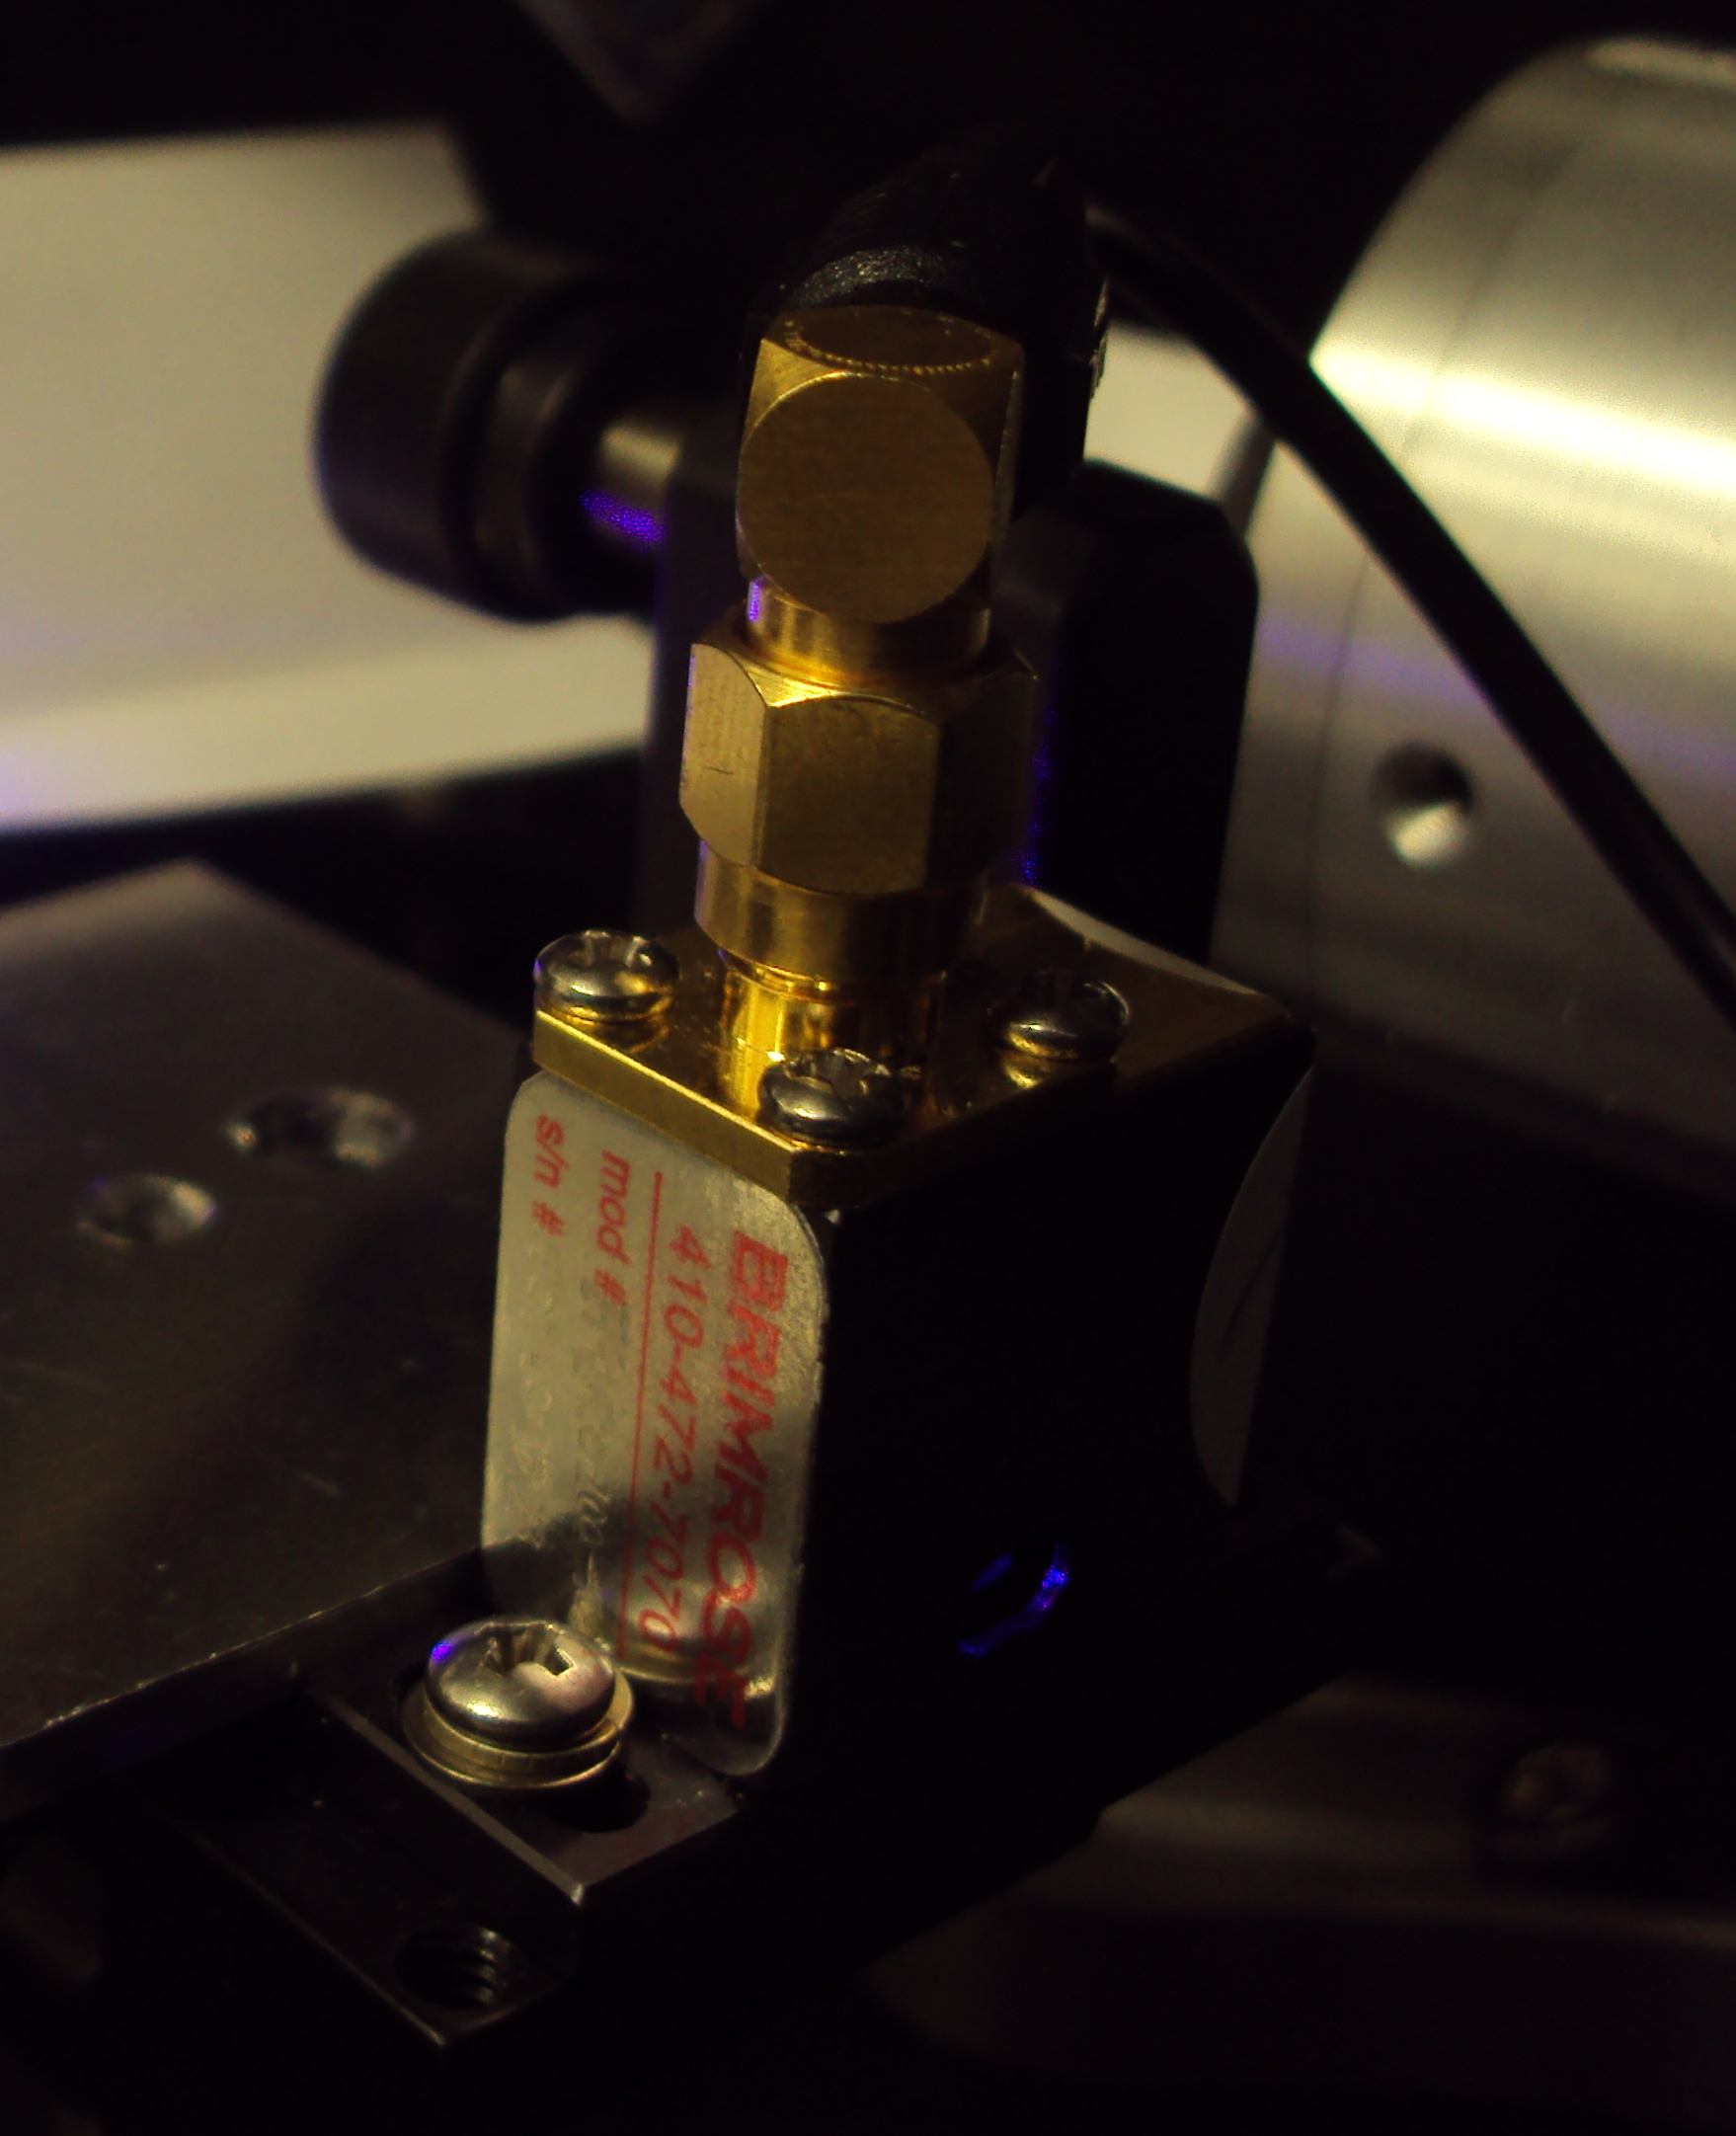
\includegraphics[width=0.95\textwidth]{aom_upclose.JPG}}
\caption[Photograph of AOM]{\label{aom_upclose} The AOM mounted in the setup. The aluminum plate in the lower left part of the photo that can be seen butting up against the AOM was used only as a guide for initial AOM alignment and was removed in the final system.}
\end{figure}
\begin{figure}
\centerline{
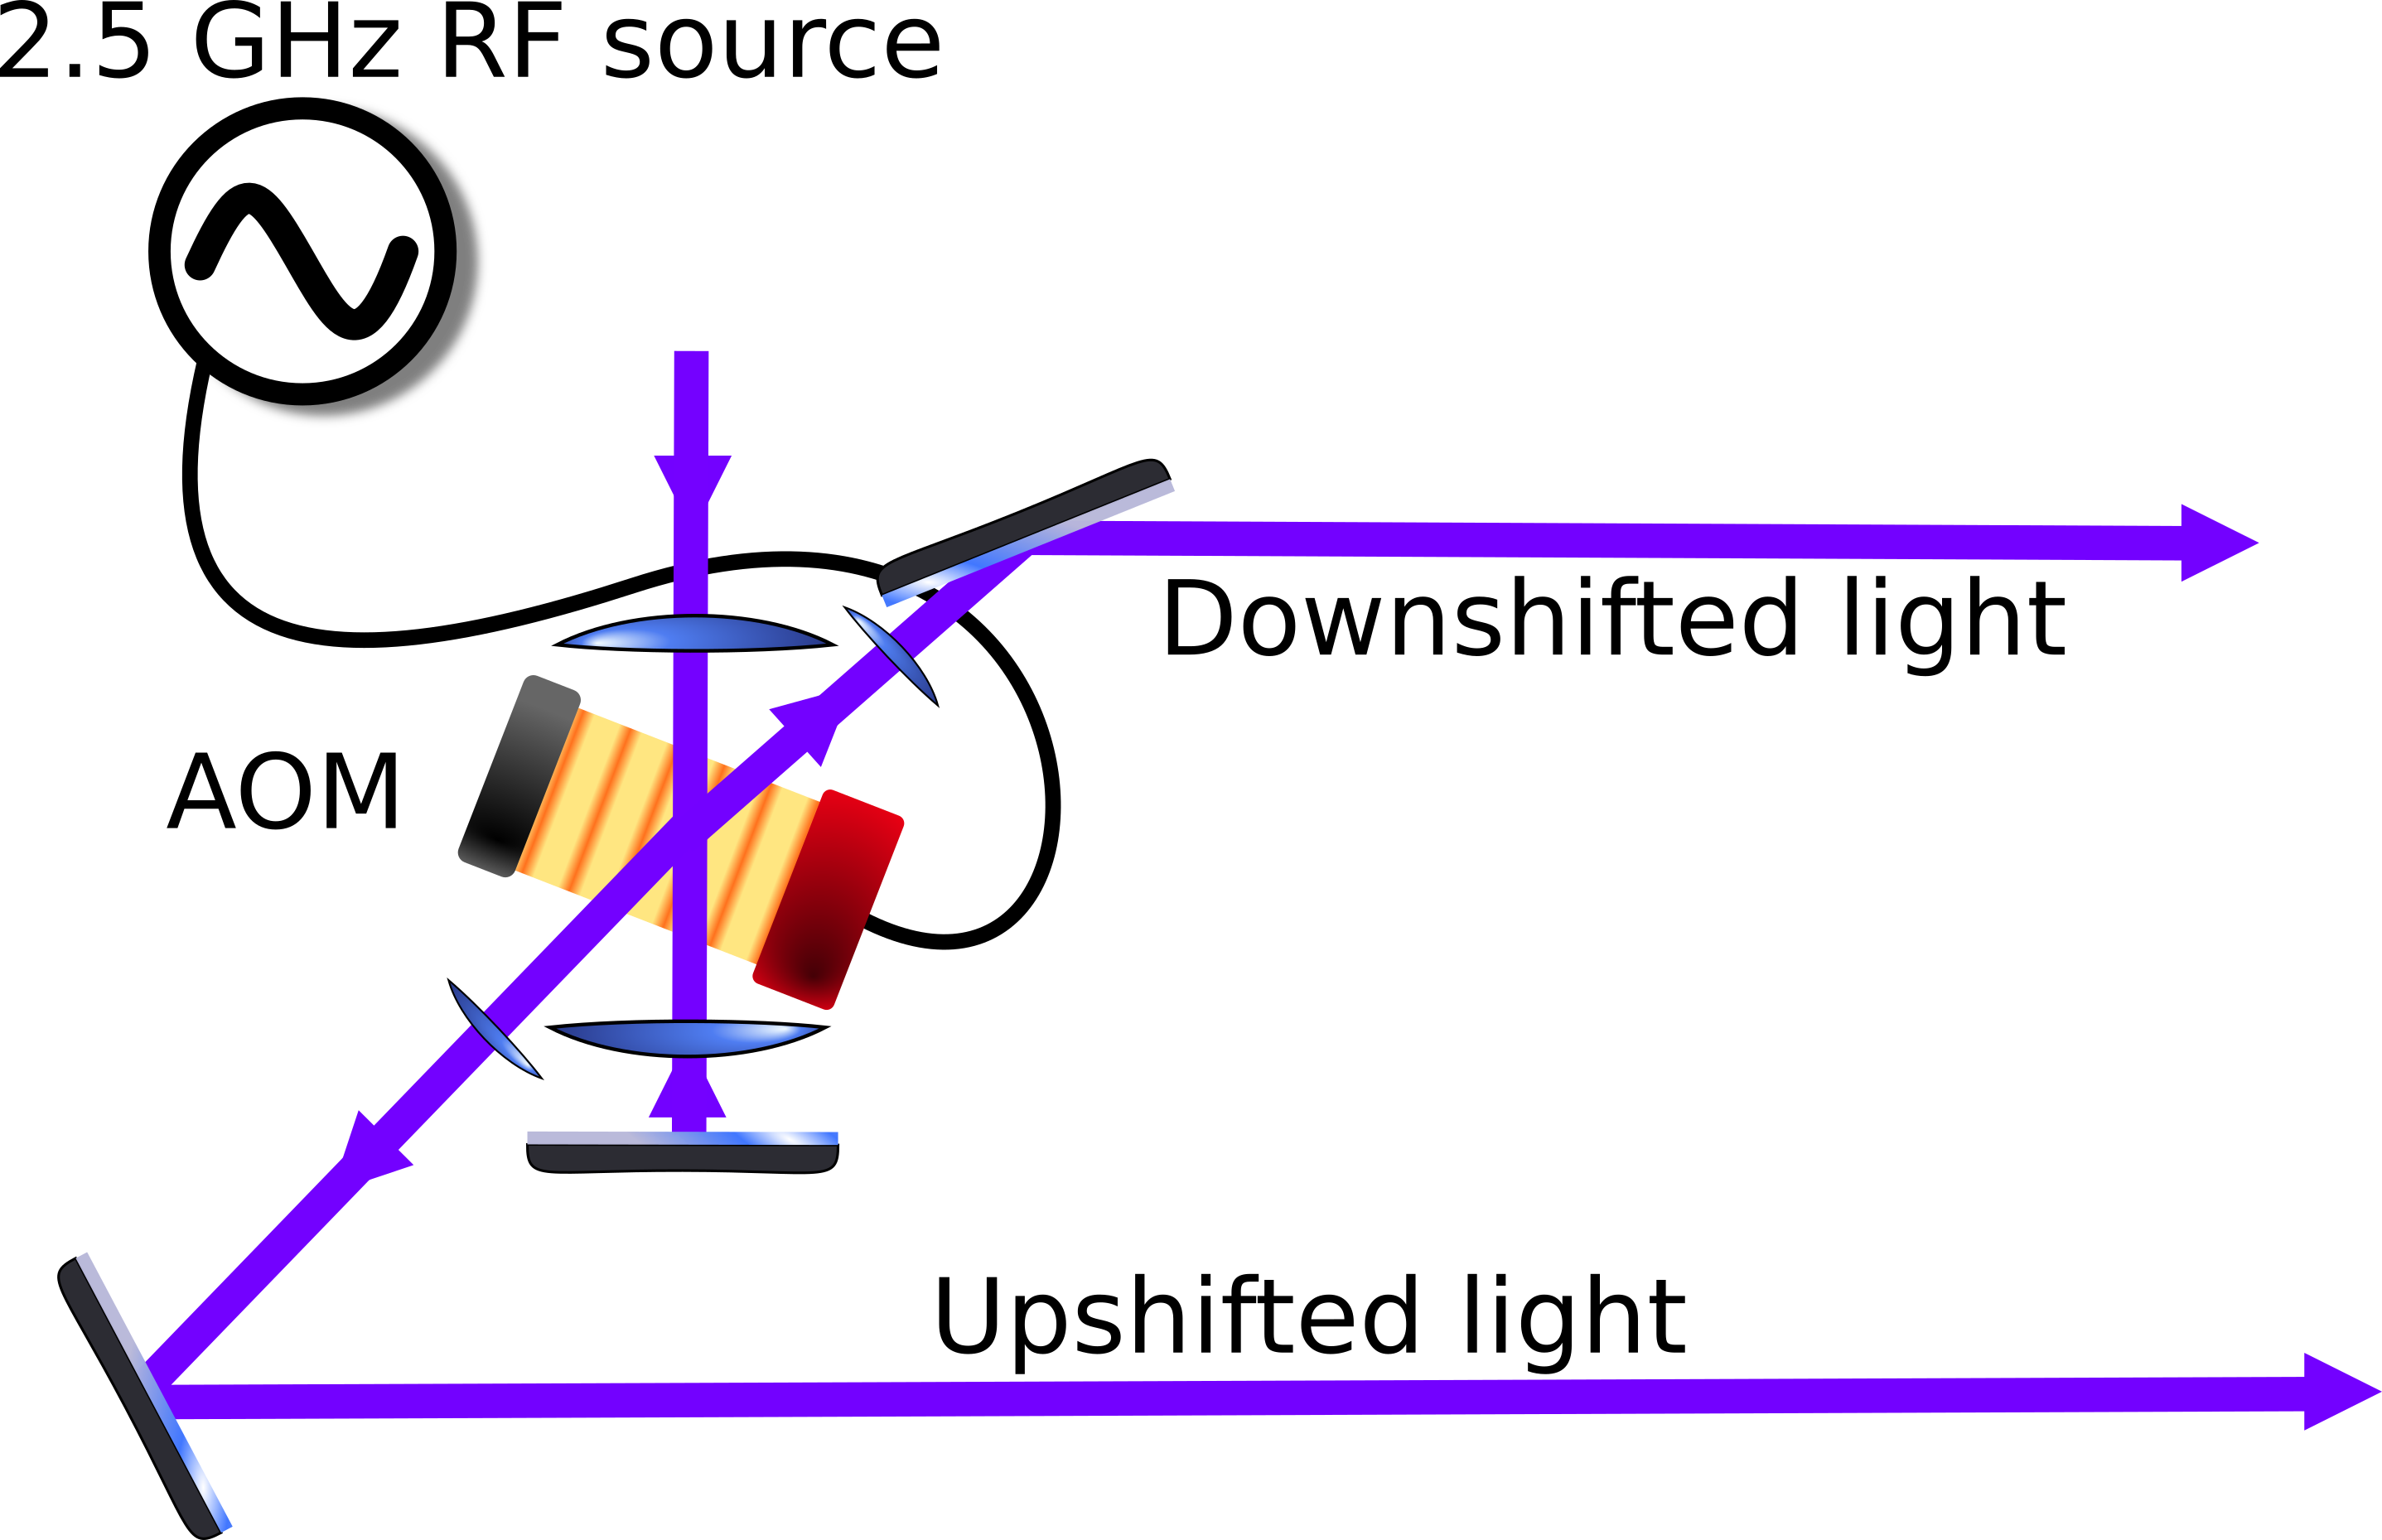
\includegraphics[width=0.95\textwidth]{diagramOfAOM}}
\caption[AOM diagram]{\label{aomDiagramDetail} Detail of Figure\,\ref{diagramOfSetup3}. The light from the master laser is depicted entering from the top of the diagram. This beam travels into the AOM, which is depicted in the center of the diagram. The up-shifted light (up-shifted in frequency, or blue shifted) is depicted travelling towards the lens and mirror near the lower left side of the diagram. The zeroth order diffracted beam is re-collimated and then retroreflected. The down-shifted light (red shifted) is depicted exiting the AOM towards the top right of the figure.}
\end{figure}

The AOM we use is model number TEF-2500-200-405 made by Brimrose Corporation of America. The crystal material is Tellurium Flouride; the center carrier frequency is 2500 MHz; the bandwidth (3dB) is 200 MHz. The AOM's anti-reflective coatings are specified to work at 405 nm. 
\section{Principle of operation}

The AOM is a crystal with a piezoelectric transducer attached to one side and an acoustic absorber attached to the other side. Acoustic waves are produced by the transducer. These waves travel across the active area of the AOM crystal and are absorbed by the absorber on the other side. The compression and decompression caused by the travelling acoustic waves changes the index of refraction within the crystal as a function of both space and time. This creates what are effectively a series of travelling Bragg planes that correspond to the acoustic wavefronts travelling across the crystal. Light crossing through the crystal can experience Bragg reflection off these planes and, because the effective reflective surface is moving, the light scattered off these features is Doppler-shifted. This light emerges at a distinct angle compared to the incoming light. This allows the AOM to produce frequency-shifted beams that are spatially separated from the unshifted components of the beam.

The relationship between the driving frequency and the Bragg angle for an AOM is well known and is given by 
\begin{equation}
m\lambda' = 2 \Lambda \sin \theta_B
%\sin{\theta}=\frac{m \lambda}{\Lambda}
\end{equation}
where $\theta_B$ is the Bragg angle (which is measured between the incoming beam and the Bragg planes), $\lambda'$ is the wavelength of the laser within the AOM crystal, $\Lambda$ is the wavelength of the acoustic wave in the crystal medium, and $m$ is an integer representing the diffraction order. The deflection angle (the angle between the unshifted portion of the beam and the outgoing shifted portion of the beam) is equal to twice the Bragg angle. Only $m=0,1$ are relevant to the experiment. The $m=1$ beams are the ones used to injection lock the slave lasers. The $m=0$ beam refers to the laser light that passes straight through the AOM with no frequency shift. Most of the power emerges in the $m=0$ diffraction order. The $m=0$ order beam from the first pass is retroreflected to produce the second pass.

The relationship between the driving frequency and the shift in the frequency of the light simply turns out to be 
\begin{equation}
    mf_{\textnormal{driving}}=\Delta f_{\textnormal{laser}}.
\end{equation}
%put in data sheet
Ultimately, getting the AOM to work properly involves optimizing just a few parameters. The AOM must be installed at the right angle relative to the incoming beam. I must ensure that as much of the incoming beam as possible hits the active aperture of the AOM, which is specified as having dimension 0.05 mm. This requires alignment in the X and Y directions, but it also means that I attempted to maneuver the AOM so that the focal point of the incoming beam was approximately in the center of the crystal in the Z direction as well (direction of propagation). This way, we keep the beam small on both of the entry holes in the case of the AOM. I also optimized the power used to drive the piezoelectric transducer. Furthermore, the intensity and shape of the incoming beam were adjusted to ensure that we do not exceed the maximum allowable intensity for the AOM, which is specified as 50 W/mm$^2$.
%shape instead of waist?
Thus, I will first discuss some work I did to characterize the incoming beam.

\section{Optimization of beam waist}
First, we would like to control the beam so that at its focus nearly all of the beam ($\sim99.96$\%) is within the active area of the AOM.
%\footnote{I did explore the possibility of just sending in a huge beam with lots of extra power in hopes that the part scattering off the active part of the AOM would work. Preliminary tests showed little promise for the technique. Furthermore, we would expect the possibility of severe distortion of the transverse mode of our laser.}
This area is specified as being 0.05 mm wide. Our goal is to have a beam waist radius that will be $\approx$4 times smaller than this 0.05 mm value.\footnote{Note that I am comparing the beam waist \emph{radius} to the full \emph{width} of the active area.} %diameter? 
If the beam waist is too small, we have to reduce the power to avoid damaging the AOM. Also, the diffraction efficiency decreases because the beam will interact with fewer Bragg planes. If the waist is too large, only a small portion of the beam would be within the active area of the AOM. This would reduce diffraction efficiency and cause distortion of the laser's transverse mode.

We can model the laser as a Gaussian beam. Gaussian beams have the property that their intensity profile always takes a Gaussian shape, i.e. \cite{lasersMilonniEberly}
\begin{equation}
\label{GaussianIntensity34}
    I(\mathbf{r})=I_0\exp\left(-\frac{2r^2}{w(z)^2}\right),
\end{equation}
where $z$ and $r$ are cylindrical polar coordinates. The variable $z$ represents position along the axis of propagation with the point $z=0$ defined to be the point along the beam path at which the beam is narrowest, while $r$ is the coordinate describing the distance from the $z$ axis. $I_0$ represents the intensity of the beam at $z=0, r=0$ and $w(z)$ is a function that gives the radius of the Gaussian beam, which is given by:
\begin{equation}
w(z)=w_0\sqrt{1+\frac{z^2}{z_R^2}}\label{beamwaist1D}.
\end{equation}
The beam radius, $w(z)$, is also the distance from the center of the beam to the point where the intensity of the beam has fallen by a factor of $1/e^2$ (i.e. the spot size). The Rayleigh range is denoted $z_R$, and also satisfies the relation 
\begin{equation}
z_R=\pi w_0^2/\lambda \label{rayleighRange1D}.
\end{equation}
A slight modification of Eq.\,\eqref{GaussianIntensity34} allows us to model elliptical beams by allowing for a different waist in each of the $x$ and $y$ directions:
\begin{equation}\label{eqForI}
    I(\mathbf{x,y})=I_0\exp\left(-2\left(\frac{x^2}{w_x(z)^2}+\frac{y^2}{w_y(z)^2}\right)\right).
\end{equation}
Here, there are two relevant beam radii, $w_x$ in the $x$ direction and $w_y$ in the $y$ direction. Each of these has an associated Rayleigh range $z_{Rx}$ and $z_{Ry}$, and each satisfies relations analogous to Eqs.\,\eqref{beamwaist1D},\eqref{rayleighRange1D}.

I can measure the Gaussian beam radius in one dimension using a standard knife-edge technique. This involves placing a photo diode in the path of the beam. A razor blade is then moved perpendicular to the beam in a controlled way such that the beam is partially blocked. The blade is then moved across the laser beam in a direction perpendicular to the blade's edge to several different locations. For each razor blade position $x$ the power incident on the photo diode is measured. By integrating Eq.\,\ref{eqForI}, we get
%picture?

\begin{equation}
{\rm Power\ incident\ on\ photodiode}=\frac{1}{2} P \left(\erf \left( \frac{\sqrt{2} x}{W_{0x}}\right)\right).
\end{equation}
%get data for this?
We do this several times at various points along the path of the laser and can perform a curve fit to calculate our beam divergence and therefore infer its waist. 

I was somewhat worried that modeling the beam coming into the AOM as a Gaussian beam would not be adequate. This was in part due to irregularities in the transverse mode of the master laser.
%\footnote{The experiment still worked -- all that matters is that we are able to get the master laser stable and couple diffracted light from the AOM into the slave lasers. Ultimately, it was discovered by other students that this was due to a manufacturing defect in the optical isolators.}
Because I was planning to operate the AOM relatively close to its damage threshold, I examined the possibility of using a more sophisticated theory to model our beam based on measurable parameters. 

Siegman \cite{SiegmanBeamQuality} discusses the characterization of beams in terms of a quantity that is known simply as ``$M^2$.'' One way to interpret $M^2$ is that it serves as a measure of how Gaussian a beam is. If a beam is Gaussian, $M^2=1$. If a beam contains higher order Laguerre-Gaussian modes, $M^2$ will be greater than 1. In Ref.\,\cite{SiegmanBeamQuality}, Siegman asserts that any beam comprised of Laguerre-Gaussian modes can be mathematically proven to propagate according to the following equation:
\begin{equation}
W_x^2=W_{0x}^2+\left( \frac{M_x^2 \,\lambda}{\pi \, W_{0x}}\right)^2 (z-z_{0x})^2 \label{SiegmanBeamPropagate01}.
\end{equation}
The $z$ coordinate of the $x$-direction beam waist is given by $z_{0x}$. The spot size parameter (radius) of the beam in the $x$ direction is represented by $W_x(z)$, which can be written as  
\begin{equation}
W_x(z)=2 \sigma_x,
\end{equation}
where the second-moment width, $\sigma_x$, is defined by 
\begin{equation}\label{secondMomentWidth}
\sigma_x^2=\frac{\int_{-\infty}^{\infty} (x-x_0)^2 I(x,y)\, dx\, dy}{\int_{-\infty}^{\infty} I(x,y)\, dx \, dy}.
\end{equation} 
Here $I(x,y)$ is the intensity profile of our beam, which is propagating in the $z$ direction. 
The second moment width $\sigma_x^2$ then satisfies the following equation:  
%shoot----this factor of 4. I might be all wrong on my calculations. 
\begin{equation}
\sigma_x^2=\sigma_{0x}^2+\left( \frac{M_x^2 \,\lambda}{4 \pi \, \sigma_{0x}}\right)^2 (z-z_{0x})^2 \label{SiegmanBeamPropagate00}.
\end{equation}
In the special case of the Gaussian beam, $2\sigma_x(z)=w_x(z)$.

In principle, we could take measurements of $\sigma_x^2$ for our beam using the knife edge technique described above at several points along the beam's path and then fit this to Eq.\,\ref{SiegmanBeamPropagate00}.
I tried allowing $M^2$ to be one of my fit parameters as I analyzed data from the beam, but I found it difficult to get data of sufficient quality to give a good estimate. The knife edge data did not have sufficient resolution over a large enough range. One problem is that the contribution to $\sigma_x$ increases as the square of the distance from the center of the beam. This means that any measurement has to be very accurately adjusted to compensate for background offset. I also attempted to use a camera, but I was not able to trust its linearity and offsets enough to get good results. Information about my attempt to calibrate the camera can be found in Appendix\,\ref{BeamWaistAppendix}. 

However, I did consider the implications on the beam if $M^2\neq 1$. I can look at the effective slope of divergence by rearranging Eq.\ \ref{SiegmanBeamPropagate00} and taking the limit as $(z-z_R) \rightarrow \infty$
\begin{equation}
\frac{\sigma_x}{z-z_R}=M_x^2 \frac{\lambda }{4 \pi \sigma_{0x}} \label{SiegmanBeamSlope}.
\end{equation}
%note: check this again. 
%does z0 matter as a fit parameter? I don't think so. 
Note that the smallest possible beam waist radius corresponding to any given beam divergence occurs if $M^2=1$. That is, if I measure the beam divergence and perform my curve fit assuming that $M^2=1$, the beam-waist radius that I calculate will be guaranteed to be \emph{smaller than or equal to} the actual beam waist radius of the beam no matter what the beam's actual value of $M^2$ might be. Thus, for the purposes of keeping the intensity at the beam waist below the AOM's damage threshold, the assumption that $M^2=1$ gives a sort of ``worst case scenario.'' 

\subsection{Ray transfer matrix analysis of system}
It is crucially important that I limit the intensity of the light that passes through the AOM. As a sanity check, I now calculate what the beam waist should be for our optical setup using an ABCD matrix (ray-transfer matrix). This model can be used to estimate the sensitivity of the system to small changes in the setup. In this way, I can verify that the system is robust against small changes and realignments and thereby gain some small reassurance. For example, if the master laser ever had to be taken apart and reassembled, it would likely be the case that there will be tiny differences in the position of the laser or collimating lens. I seek to verify that such small changes will not yield catastrophic changes in the size of the beam as it passes through the AOM.  

%This is in a lab notebook somewhere. You need to find it there, I think. Or it's in a Mathematica file. 
%found: the Mathematica files are generalABCDfinding.nb, ABCDwillWeBreakAOM.nb . The m files, well, I think the ones I want are in checkTheWaists_realDATA. 

There is a method of modeling Gaussian beam propagation using a matrix
\begin{equation}
M=\begin{bmatrix}A&B \\C&D\end{bmatrix}
\end{equation}
which is known as a ``ray transfer matrix'' or simply as an ``ABCD matrix.'' We will use the well-known rule \cite{BYUOpticsBook}\cite{lasersMilonniEberly} for modelling a Gaussian beam as it passes through a system described by a ray transfer matrix with elements $A$,$B$,$C$ and $D$, which is 
\begin{equation} \label{ABCDlawforGaussianBeams}
z_0'-iz_R'=\frac{A(z_0-iz_R)+B}{C(z_0-iz_R)+D}.
\end{equation}
Here, $z_0'$ represents the location of the beam waist relative to the end of the system described by the ABCD matrix and $z_R'$ represents the new Rayleigh range of the beam. The location of the beam waist relative to the start of the system described by the ABCD matrix and the Rayleigh range of the incoming beam are represented by $z_0$ and $z_R$ respectively.
This can be solved to give 
\begin{align}
z_R' &= \frac{ z_R (BC-AD)}{C^2z_0^2+C^2z_R^2+2 C D z_0 + D^2} \\
z_0' &=\frac{AC z_0^2+ACz_R^2+ADz_0+BCz_0+BD}{C^2z_0^2+C^2z_R^2+2 C D z_0 + D^2}.
\end{align}
(Note that in an ABCD matrix, $A$ and $D$ are unit-less, while $B$ has units of $[\textnormal{length}]$, and $C$ has units of $[\textnormal{length}]^{-1}$.)

%This calculation should give us a feel for how sensitive we are to drifts in the optical setup. We will also be able to verify that the beam waist near the AOM is close to what we would expect based on the beam waist at the laser diode.

The system has only a few components that we need to model. At the start, we assume that the light coming out of the face of the laser diode is essentially a Gaussian beam with different beam waist radii for the $x$ and $y$ directions. The waist of this beam can be estimated based on parameters given in the data sheet. The data sheet for the master laser shows that a typical angle of divergence for light coming out of the laser is going to be 9$^\circ$ in one direction and 19$^\circ$ in the other. A Gaussian beam's angular divergence can be surmised by looking at Eq.\ \ref{SiegmanBeamSlope}. The relationship turns out to be the one given in Ref.\,\cite{MellesGriotGaussian}:
\begin{align}
\theta_{x} &= \frac{\lambda}{\pi w_{0x}}\\
\theta_{y} &= \frac{\lambda}{\pi w_{0y}}.
\end{align}  
Using this equation, we calculate the equivalent Gaussian beam height and width at the face of the laser based on the given angle of divergence of light. The beam waist dimensions turn out to be 972.913 nm and 460.854 nm at the face of the laser.

The light from the laser head is emitted and collimated by a lens\footnote{Thorlabs C570TM-A} with focal length 2.84 mm.  %before, I had 2.87 mm, IDK why
The propagation of the light from the laser diode to the collimating lens can be represented by the matrix
\begin{equation}
\begin{bmatrix}\label{ABCD1}
1 & d_1 \\ 0 & 1
\end{bmatrix},
\end{equation}
where $d_1$ represents the distance between the face of the laser and the collimating lens. The effect of the collimating lens is represented by the following ABCD matrix:
\begin{equation}
\begin{bmatrix}\label{ABCD2}
1 & 0 \\ -1/f_{a} & 1
\end{bmatrix}.
\end{equation}
Here, $f_a\approx$ 2.84 mm is the focal length of the lens

The beam then goes through various optical components, including the diffraction grating, the optical isolators, some wave plates, a polarizing beam cube, and many mirrors. The collective impact of these components on the waist of the beam can be modeled as simple propagation over some effective distance. %Even though propagating through a medium like the crystals in the optical isolators is different than propagating through air, travelling some distance through any medium is represented by the same ray transfer matrix as travelling some effective distance through air. 
In order to be complete, I will evaluate the outgoing beam properties over the entire range of possible path lengths. This is much easier than trying measure the total path length accurately and then trying to find detailed dimensions and indices of refraction for all the components in the system. The ABCD matrix representing this propagation is given by
\begin{equation}
\begin{bmatrix}\label{ABCD3}
1 & d_2-d_1 \\ 0 & 1
\end{bmatrix},
\end{equation}
where $d_2$ represents the total distance the beam travels from the face of the laser diode up until it reaches the lens that focuses it into the AOM. Thus, $d_2-d_1$ represents the distance from the collimating lens of the master laser to the lens that focuses the beam into the AOM. 
I estimate that the effective distance of propagation should be on the order of 1 m. To be safe, I will ultimately examine what happens for all beam paths between 0.5 m and 2 m. 

Finally, the beam is focused by a lens with focal length 10 cm and passed through the AOM. The focusing of the 10cm focal length lens is represented by
\begin{equation}
\begin{bmatrix}\label{ABCD4}
1 & 0 \\ -1/f_{f} & 1
\end{bmatrix},
\end{equation} 
where the focal length of the lens is written as $f_{f}$.

We can write the ABCD matrix for the whole system as the product of the ABCD matrices that represent the individual components of the system that were found in Eqs.\,\eqref{ABCD1},\eqref{ABCD2},\eqref{ABCD3}, and \eqref{ABCD4}: 
\begin{equation}\label{ABCDMatrixSystem}
\begin{bmatrix}
1 & 0 \\ -1/f_{f} & 1
\end{bmatrix}
\begin{bmatrix}
1 & d_2-d_1 \\ 0 & 1
\end{bmatrix}
\begin{bmatrix}
1 & 0 \\ -1/f_{a} & 1
\end{bmatrix}
\begin{bmatrix}
1 & d_1 \\ 0 & 1
\end{bmatrix}
=
\begin{bmatrix}
A & B \\ C & D
\end{bmatrix}.
\end{equation}

Finding the resulting ray transfer matrix that describes the system involves simply performing the matrix multiplication prescribed in Eq.\,\ref{ABCDMatrixSystem}. However, I opt not to write out result in this thesis. Instead, I used Mathematica to find the expressions for $z_R'$ and $z'$. These expressions were then evaluated numerically for several values of likely experimental parameters. In particular, I was interested in verifying that the beam waist inside the AOM remains reasonable for realistic values of $d_1$ (the distance from the laser face to the collimating lens) and $d_2$ (the distance traveled between the collimating lens and the other lens), since these are values that may not be known to high precision and which may drift with time. %may change as the system is maintained or repaired.

From this analysis, I calculated the effective area of the beam for many values of $d_1$ and $d_2$. For each of these values, I calculated the corresponding ratio between the intensity at the most intense part of the beam and the total power in the beam. The way to interpret this is that if we have a constant amount of power, the ratio shows how much the maximum intensity of the beam changes for different beam parameters. The data in Fig.\,\ref{waists111} shows that the maximum intensity of the beam changes smoothly as a function of $d_2$ and that for small drifts in $d_2$, the changes in the beam's maximum intensity are reasonable. 
%what about the position of the minimum? 
%If the calculations are correct, %what am I? A cartoon? 
Figure\,\ref{waists2} shows a plot of the effective area of the beam as a function of $d_1$ (the distance from laser face to collimating lens). The effective area is given by the expression $\pi W_{0x}W_{0y}/2$. The intensity at the center of the beam waist, $I_{max}$ is given by $I_{max}=\textnormal{power}/\textnormal{effective area}$. Figure\,\ref{waists2} shows that the effective area of the beam is sharply peaked when $d_1=f_a$, which means that the intensity is at a local minimum. If we assume that the laser was reasonably well-collimated when we did the initial optimization, we can deduce that the intensity of the laser at its focus will increase if the distance $d_1$ were to drift in the actual setup. Thus, any adjustment to $d_1$ should be accompanied by a reassessment of the power and waist of the beam hitting the AOM. The extent to which the beam is collimated can be evaluated visually by shining the beam on a wall that is about $\sim$1 m away. The collimating lens on the laser is mounted on a mount that fits into a 40 turns/inch threaded hole. Adjustments to the collimation are made by turning the lens holder.  Based on my experience collimating the laser, I am relatively confident that I can get the lens holder to within 1/10 of a turn of where it needs to be to collimate the laser perfectly.  An accuracy of 1/10 turn corresponds to getting the distance $d_1$ to within 0.010 mm of the focal length of the collimating lens. Clearly, this places $d_1$ somewhere within the main spike on the plot in Figure\,\ref{waists2}, but it does not lend enough confidence in the repeatability of this adjustment to allow an experimenter to forego reassessing the beam parameters at the AOM. 

\begin{figure}
    %\centerline{\includegraphics[trim=100pt 100pt 100pt 100pt, clip=true, totalheight=0.5\textheight,angle=90]{testfigure}}
    %\centerline{\includegraphics[totalheight=0.3\textheight]{testfigure}}
    \centerline{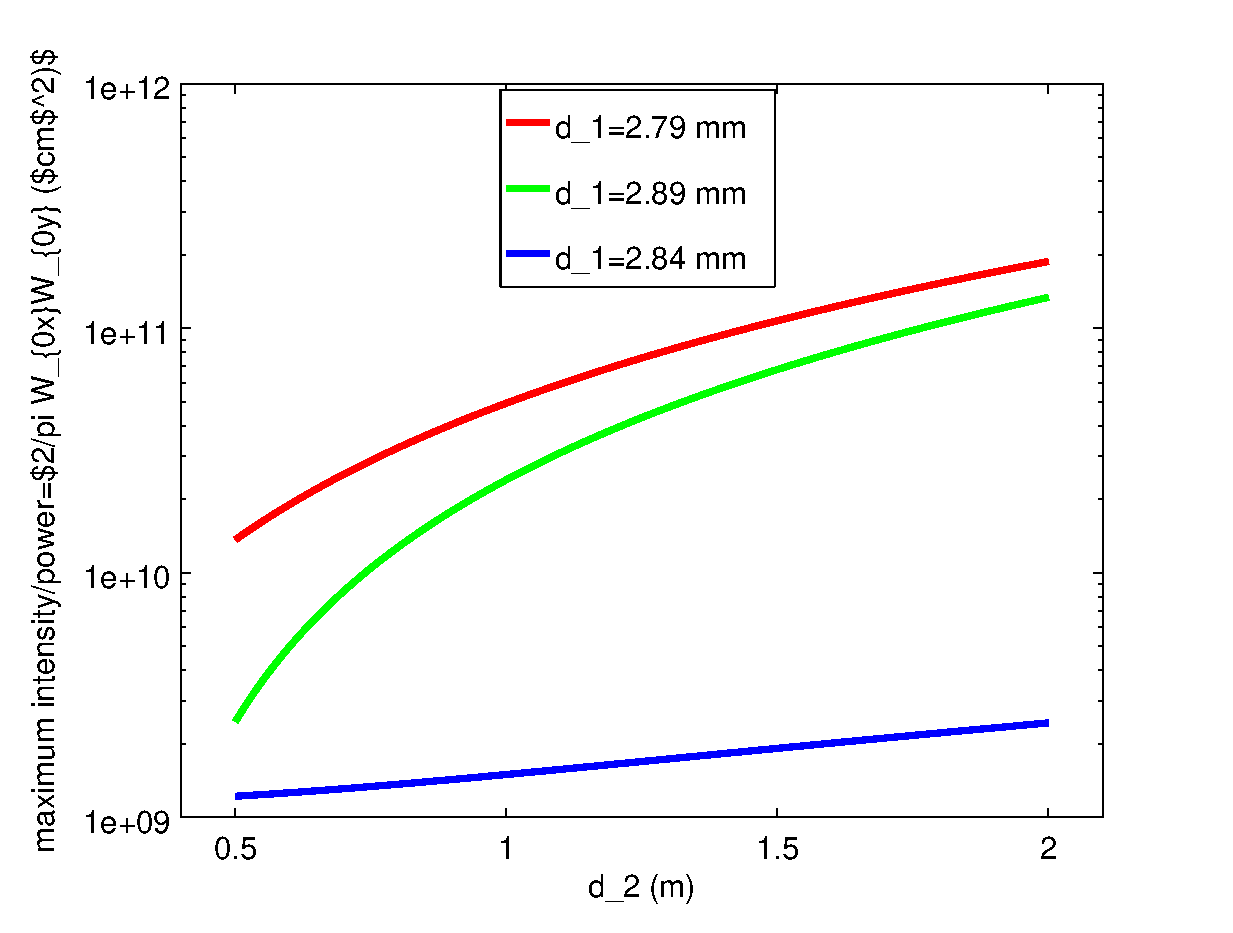
\includegraphics[width=0.95\textwidth]{waists1.eps}}
    %\includegraphics[totalheight=0.3\textheight]{testfigure}
    \caption[Maximum intensity$/$total beam power vs distance]{\label{waists111} The ratio of the maximum intensity to the total beam power as a function of the distance between the laser's collimating lens and the focusing lens ($d_2$) plotted for several values of $d_1$, which is the distance between the laser diode's output face and the collimating lens. The maximum intensity divided by the total beam power is given by $2/(\pi W_{0x}W_{0y})$. Because it is difficult to measure $d_2$ accurately, we have plotted it over a very large range of possible values. However, the actual path length is likely to stay the same to within a few millimeters, over which scales the system is relatively insensitive to changes in $d_2$.} 
\end{figure}
%%%%%TODO FIX CAPTION D2 IS IN m NOT mm

\begin{figure}
    %\centerline{\includegraphics[trim=100pt 100pt 100pt 100pt, clip=true, totalheight=0.5\textheight,angle=90]{testfigure}}
    %\centerline{\includegraphics[totalheight=0.3\textheight]{testfigure}}
    \centerline{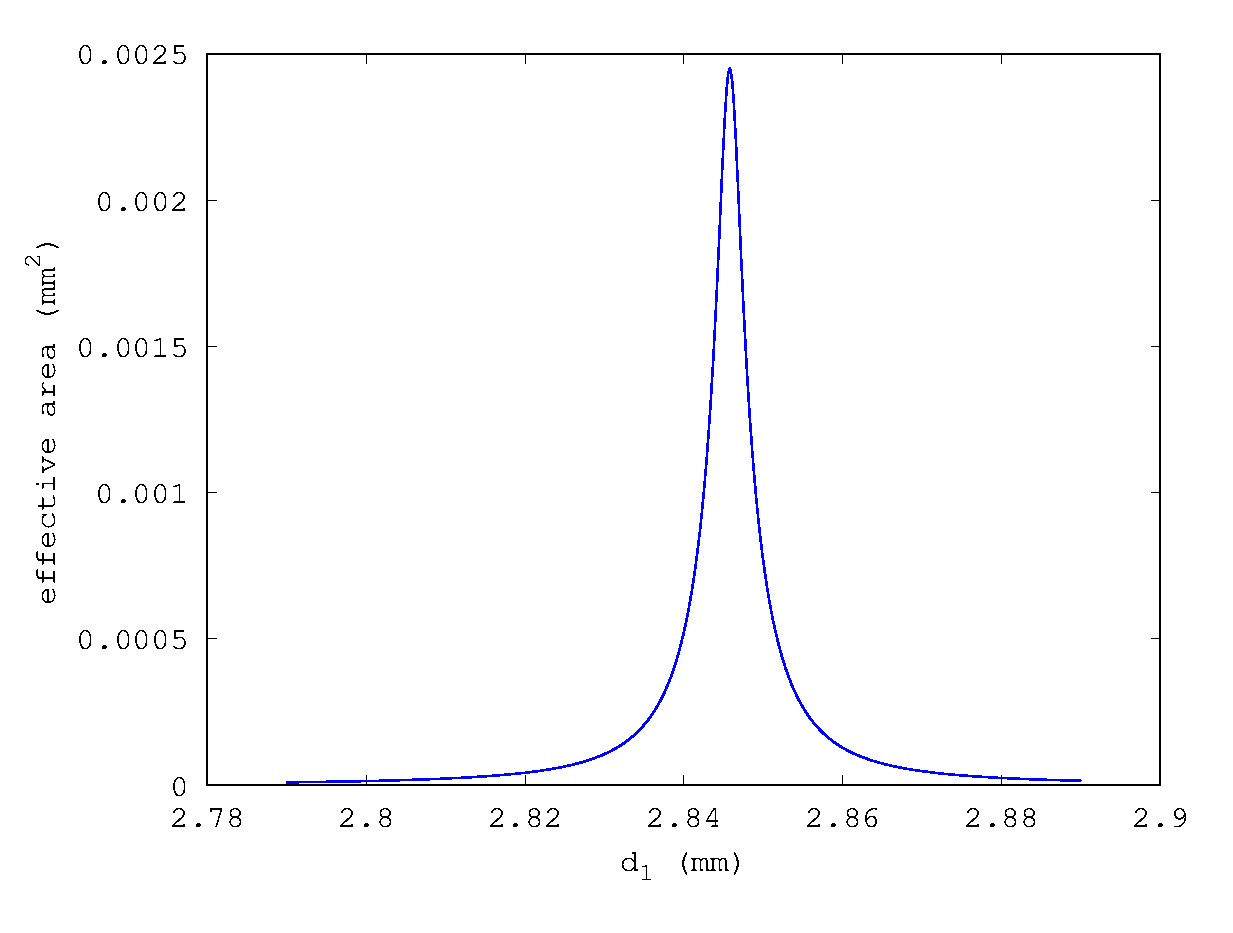
\includegraphics[width=0.95\textwidth]{waists2.eps}}
    %\includegraphics[totalheight=0.3\textheight]{testfigure}
    \caption[Effective beam area vs distance]{\label{waists2}
        The effective beam area at the beam's focus as a function of the distance between the laser diode's output face and the collimating lens ($d_1$).  Here, it is clear that the effective area is largest when $d_1$ equals the focal length of the laser's collimating lens. The peak intensity gets larger with any change of $d_1$.}
\end{figure}

 \chapter{Injection Locking}\label{InjectionLockingChapter}
 %(mode matching, measuring photocurrent from lasers, details of optimizing the isolators, some important caveats about not letting the wrong light couple back into the other laser. 


In order to achieve injection locking, we must couple the first order diffracted light that came out of the AOM into the laser cavities of each of the slave lasers. In this way, we seed the slave lasers, thereby ensuring that they will be coupled to the master laser. Additionally, the current and temperature of the slave lasers must be adjusted so that they are ``happy'' operating at that wavelength. ``Happy'' is the colloquial way to refer to the fact that for any given wavelength, the laser will give prolonged, single-mode operation only for certain combinations of temperature and current. 
Injection locking two slave lasers was necessary to get more power than would have been available from just the shifted beams from the master laser alone. 

\section{Theory of operation}

%why did this work at all? How did we know how much light would work? 

The laser operates on the principle of stimulated emission of radiation. In a non-injection-locked laser, the laser's output is determined by the interplay of several factors, including the resonant modes of the laser cavity and the spectral characteristics of the laser gain medium.
``Mode competition'' is the process whereby the power circulating in the laser concentrates in certain, more dominant modes at the expense of others. Since the gain saturation of the diode laser is determined largely by the rate at which electron-hole pairs can be created, it is possible for one mode to dominate the other modes by reaching not only self-saturation, but cross-saturating the gain medium for the other modes\cite{RPPhotonicsEncyclopediaAndBuyersGuide}. This results in essentially single mode operation. 

Therefore, intuitively, the goal of injection locking is to merely couple enough light into a suitable mode of the slave laser so that this mode has a slight advantage over the other modes. 

%did this stuff even work? 
\section{Initial slave configuration}
\label{initialSlaveConfiguration}


I selected the slave lasers in a similar way to how I selected the master laser. I used the wavelength-selected diodes with the data I took on the Ocean Optics spectrometer. The setup and configuration of the slaves was very similar to what I did with the master laser, including all the part numbers and control electronics as described in Chapter\,\ref{masterLaserDiodes}. The slave lasers, however, have no diffraction grating. Rather than using grating feedback, the slave lasers achieve improved stability and wavelength control because they are injected with shifted light from the AOM, whose stability is determined by the stability of the master laser and the rf oscillator that drives the AOM. 

%can I use the diffraction grating with seed light? 


%Notice that there was something about stray light reflections that we had to be careful of, I think. 

\section{Matching the mode properly}
I optimized coupling to the laser diode by using the following technique: First, I turned off the slave lasers and disconnected them from their current supplies. Next, I used the slave laser diode as a photodiode. I coupled light from the AOM into the laser and measured the photocurrent produced by the laser. Better coupling between the beam from the AOM and the laser results in higher photocurrent coming out of the laser. In this way, I can conveniently align the optics. 
%In order to couple to the slave lasers, we used the following technique: was that we detached the lasers from their current supplies and then used the lasers 
%For Slave 1, the half-intensity angle was rated to be 9$^\circ$ in the direction parallel to the polarization. and 19$^\circ$ in the perpendicular direction. 

I also adjusted the temperatures of the lasers in order to maximize the range of currents over which they would stay injected. 
When slave 2 was injection locked, the current produced when coupling the light in from the AOM was 8.2$\mu$A. The current at which it was working was 71.752 mA %(27292 counts on the digital controller) 
and the temperature was found to be 311.309K. %(59112 counts on the digital controller)\footnote{Lab Notebook section V page 66}.
Slave 1 worked properly at XXXXXXX TODO: FIND THIS.

The amount of power being sent towards each slave (though, not necessarily being coupled in) is $\sim$90$\mu W$. The slaves typically produce 48 mW - 63 mW.




\chapter{Results and Conclusions}\label{triumphantDataChapter}

The injection locking was successful and I successfully produced two working beams with an adjustable detuning. I have verified that both beams' frequencies are coupled to and offset from the master laser. Furthermore, the output from the slaves is sufficient to drive the transition. 

\section{Brief note on data from the spectrum analyzer}

The main way that we can see if the lasers are working properly is to couple them to the spectrum analyzer, which was discussed in Section\,\ref{spectAnalayzer} and Appendix\,\ref{SpectrumAnalyzerAppendix}. The spectrum analyzer is an optical cavity whose length is being changed as a function of time. A photo diode on the end of the spectrum analyzer captures a signal that is proportional to the transmission through the spectrum analyzer cavity. This signal is read on an oscilloscope.

For all of the data in this thesis, the length of the spectrum analyzer was modulated in a sawtooth pattern. Thus, the length of the cavity changed at a constant speed over some interval before being quickly brought back to its original length. A typical scan typically involves changing the length of the cavity by $\sim$3$\mu$m. 

%todo: put in a picture of the cavity

The output of the photo diode is sent to an oscilloscope that is triggered by the frequency generator that also modulates the piezoelectric actuators on the spectrum analyzer. Therefore, typical data from the spectrum analyzer is a trace from an oscilloscope. The $y$ axis represents signal from the photo diode, while the $x$ dimension represents time elapsed since the last triggering event. The $x$ axis values in the regimes shown in Figures\,\ref{fig:slaveMaster} and \ref{fig:typicaldata} are also proportional to the change in length of the cavity because the cavity length is changing linearly as a function of time during the parts of the scan that I am showing. Because each sweep of the sawtooth function generator and piezo driver is identical, we can safely compare subsequent traces to track the relative frequency changes of any given peak. 

If we scan about $\sim$2$\mu$m, we expect that the peaks corresponding to our 408 nm lasers will go in in and out of resonance $\sim$5 times. Therefore, we would expect that in the oscilloscope trace, the same peak should be repeated approximately five times. For this cavity, the free spectral range is 187 MHz. This means that the distance between two peaks from the the same spectral component of the light in our scan will correspond to the distance that any given peak would move by if it were detuned by 187 MHz. This gives us a natural scale by which to judge the movement of peaks. 

However, note that the detunings relevant to this experiment are on the order of GHz, which is much larger than the free spectral range of the cavity. This simply means that two nearby peaks coming from different lasers are from different modes of the spectrum analyzer. 

%fsr corresponds to different lengths for different lasers 

\section{Tracking slave lasers with master laser}

First, when we look at one slave and the master laser on the spectrum analyzer and scan the master laser, we see that the slave scans with the master laser. This is illustrated in Figure\,\ref{fig:slaveMaster}.

\begin{figure}
    %\centerline{\includegraphics[trim=100pt 100pt 100pt 100pt, clip=true, totalheight=0.5\textheight,angle=90]{testfigure}}
    %\centerline{\includegraphics[totalheight=0.3\textheight]{testfigure}}
    \centerline{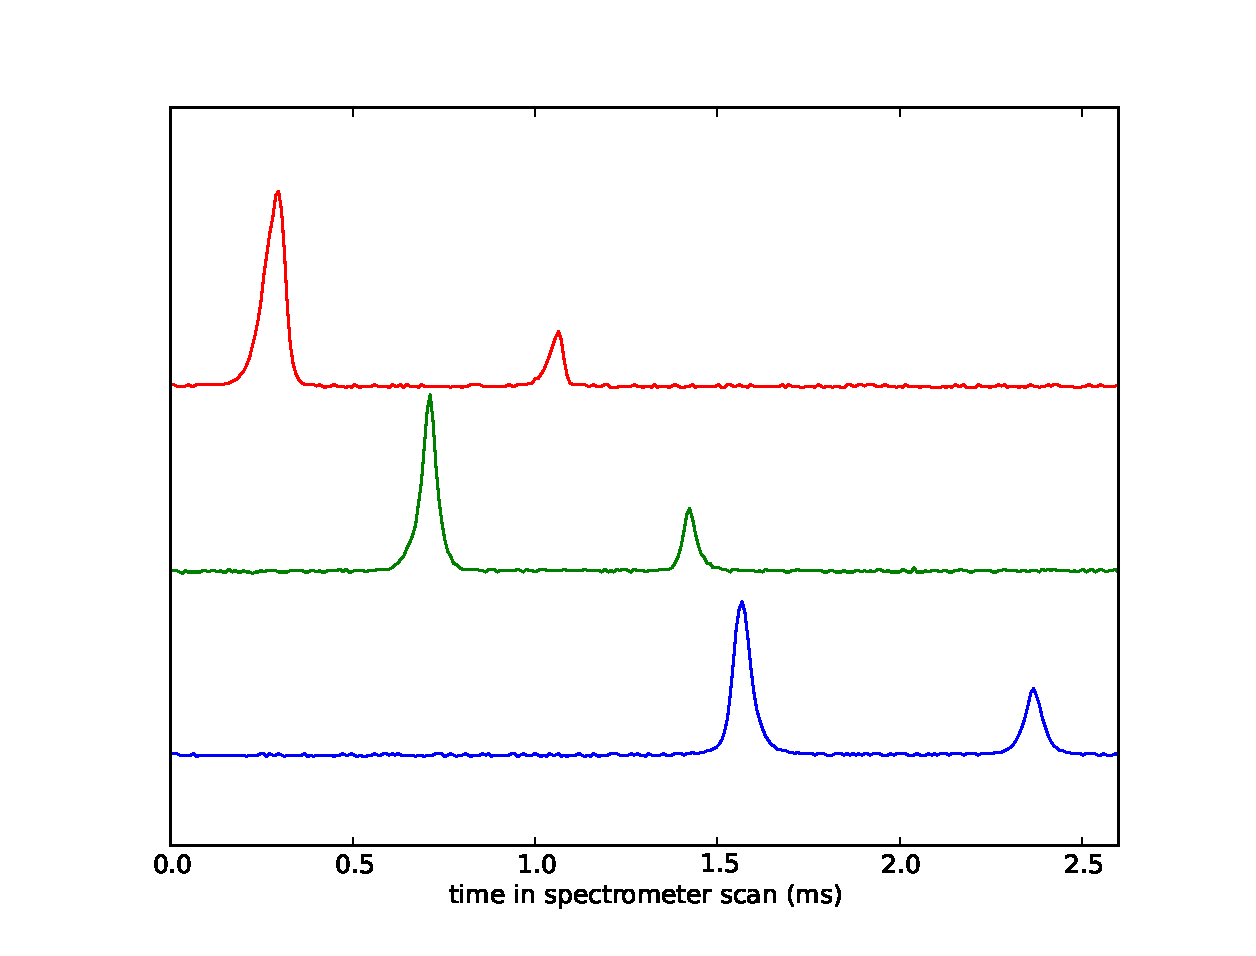
\includegraphics{Slave2AndMasterScanningMaster}}
    %\includegraphics[totalheight=0.3\textheight]{testfigure}
    \caption[Slave laser and master laser frequencies tracking together]{\label{fig:slaveMaster}
    The slave and master laser on the spectrum analyzer. The y axis is the signal on the spectrum analyzer. There are three traces here, each showing the master laser at a different frequency. The slave laser is the taller peak, while the other peak belongs to the master laser. The peaks corresponding to the master laser and the slave laser move together. Each trace is offset in the $y$ direction in order to make it visible.}
\end{figure}

\section{Verifying that the slave frequencies can be adjusted with the RF oscillator}
Second, I examined the output of the spectrum analyzer while both slave lasers were coupled into it. 
The two peaks clearly corresponded to the two slave lasers, which we verified by alternatively blocking each of the slaves. 

%We can see that there is a lot of power 

I performed an experiment where I adjusted the driving frequency of the rf frequency generator that drives the AOM. I observed that the peaks on the spectrum analyzer shifted by an amount corresponding to the change in the frequency of the rf oscillator. This provides strong evidence that the two slaves were, indeed, injection locked to the modulated beams coming out of the AOM. This data is presented in Figure\,\ref{fig:typicaldata}.


%where is the energy going? I think it goes from reflecting to transmitting
%I'm curious about finding the contribution to the line width of the cavity from the peaks.
 
\begin{figure}
    %\centerline{\includegraphics[trim=100pt 100pt 100pt 100pt, clip=true, totalheight=0.5\textheight,angle=90]{testfigure}}
    %\centerline{\includegraphics[totalheight=0.3\textheight]{testfigure}}
    \centerline{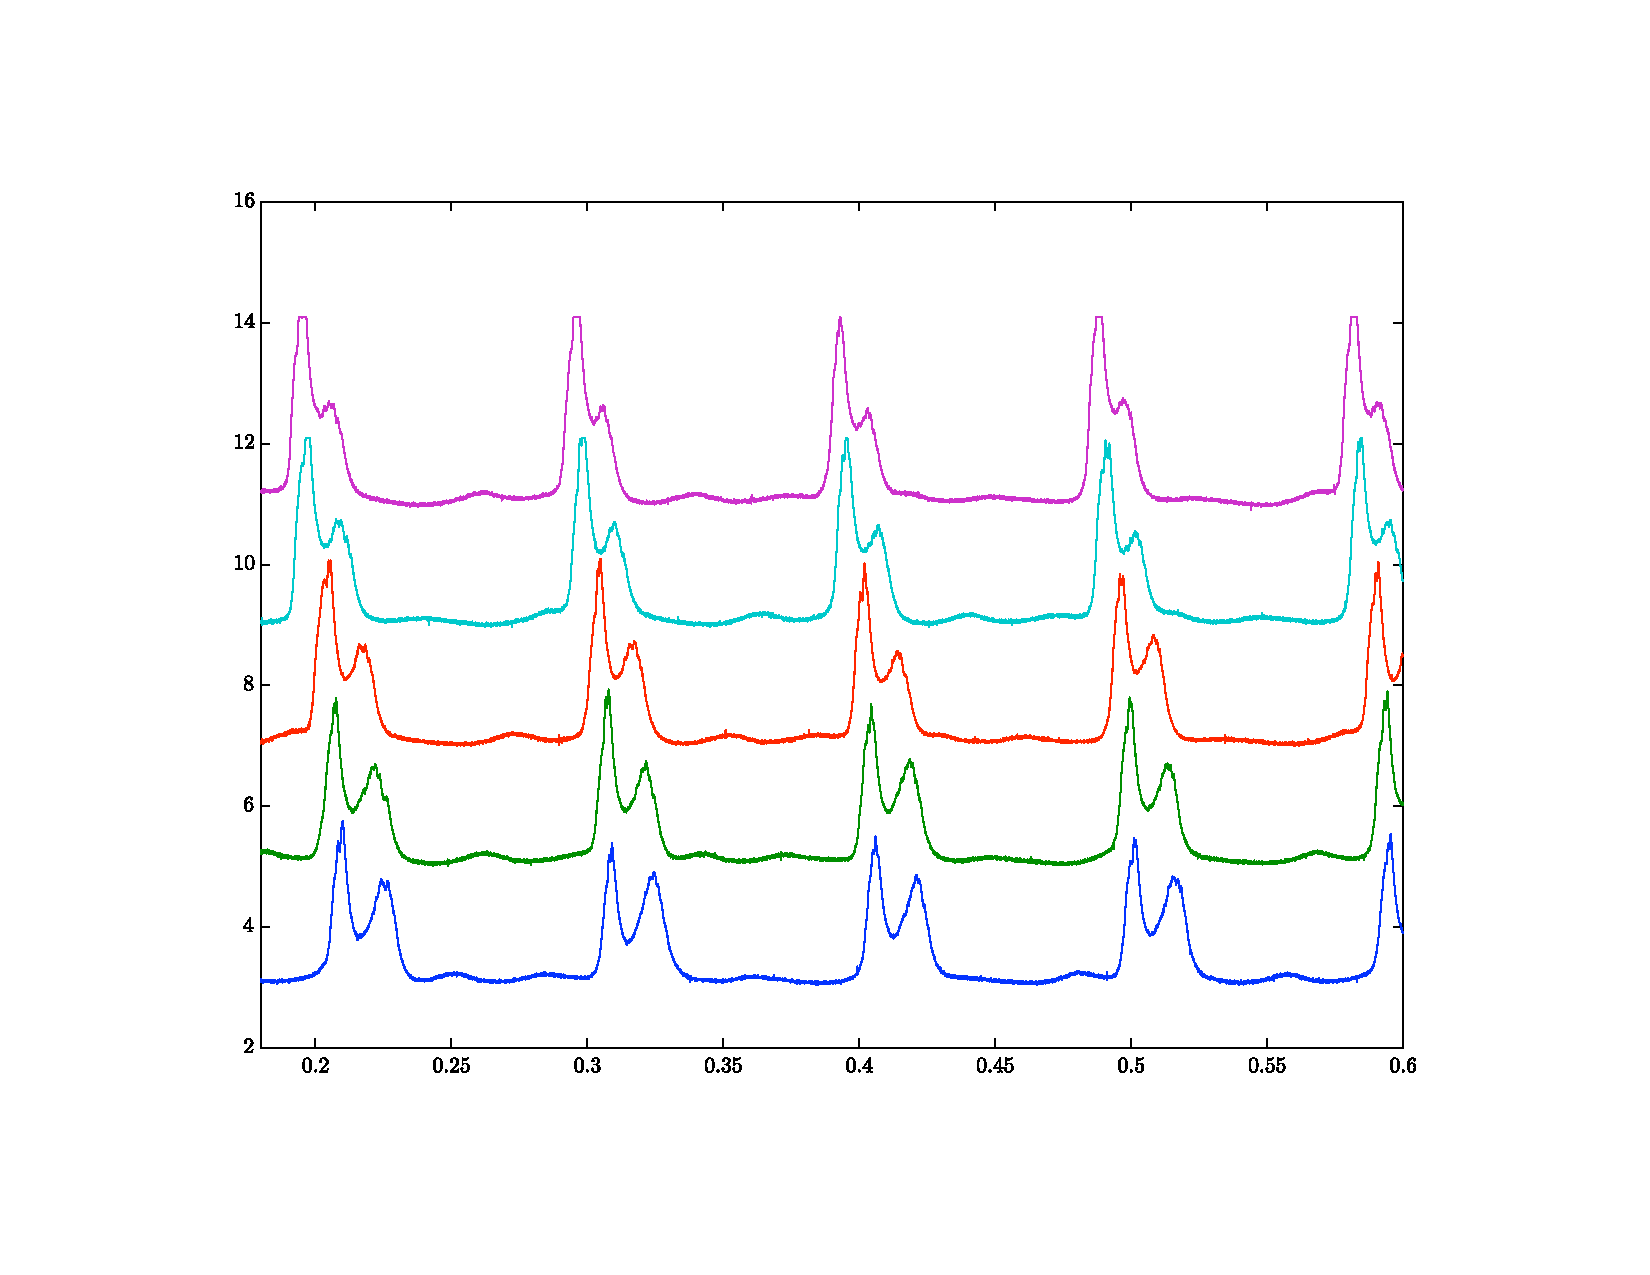
\includegraphics[width=0.9\textwidth]{sampleOffsetData}}
    %\includegraphics[totalheight=0.3\textheight]{testfigure}
    \caption[Scans of slave lasers for several rf oscillator frequencies]{\label{fig:typicaldata}
Scans of slave lasers for several rf oscillator frequencies. I changed the detuning on the frequency generator in 10 MHz increments between capturing each of these traces. The $y$ axis represents transmission through the spectrum analyzer cavity as measured by the photo diode and is presented in arbitrary units with the traces offset to enhance visibility. The $x$ axis represents time during the cavity scan. As the detuning changes, the distance between the two peaks shifts, thereby proving that the detuning between the slave laser and the master laser is controlled by the AOM and rf frequency generator.}
\end{figure}

%\begin{figure}
%\centerline{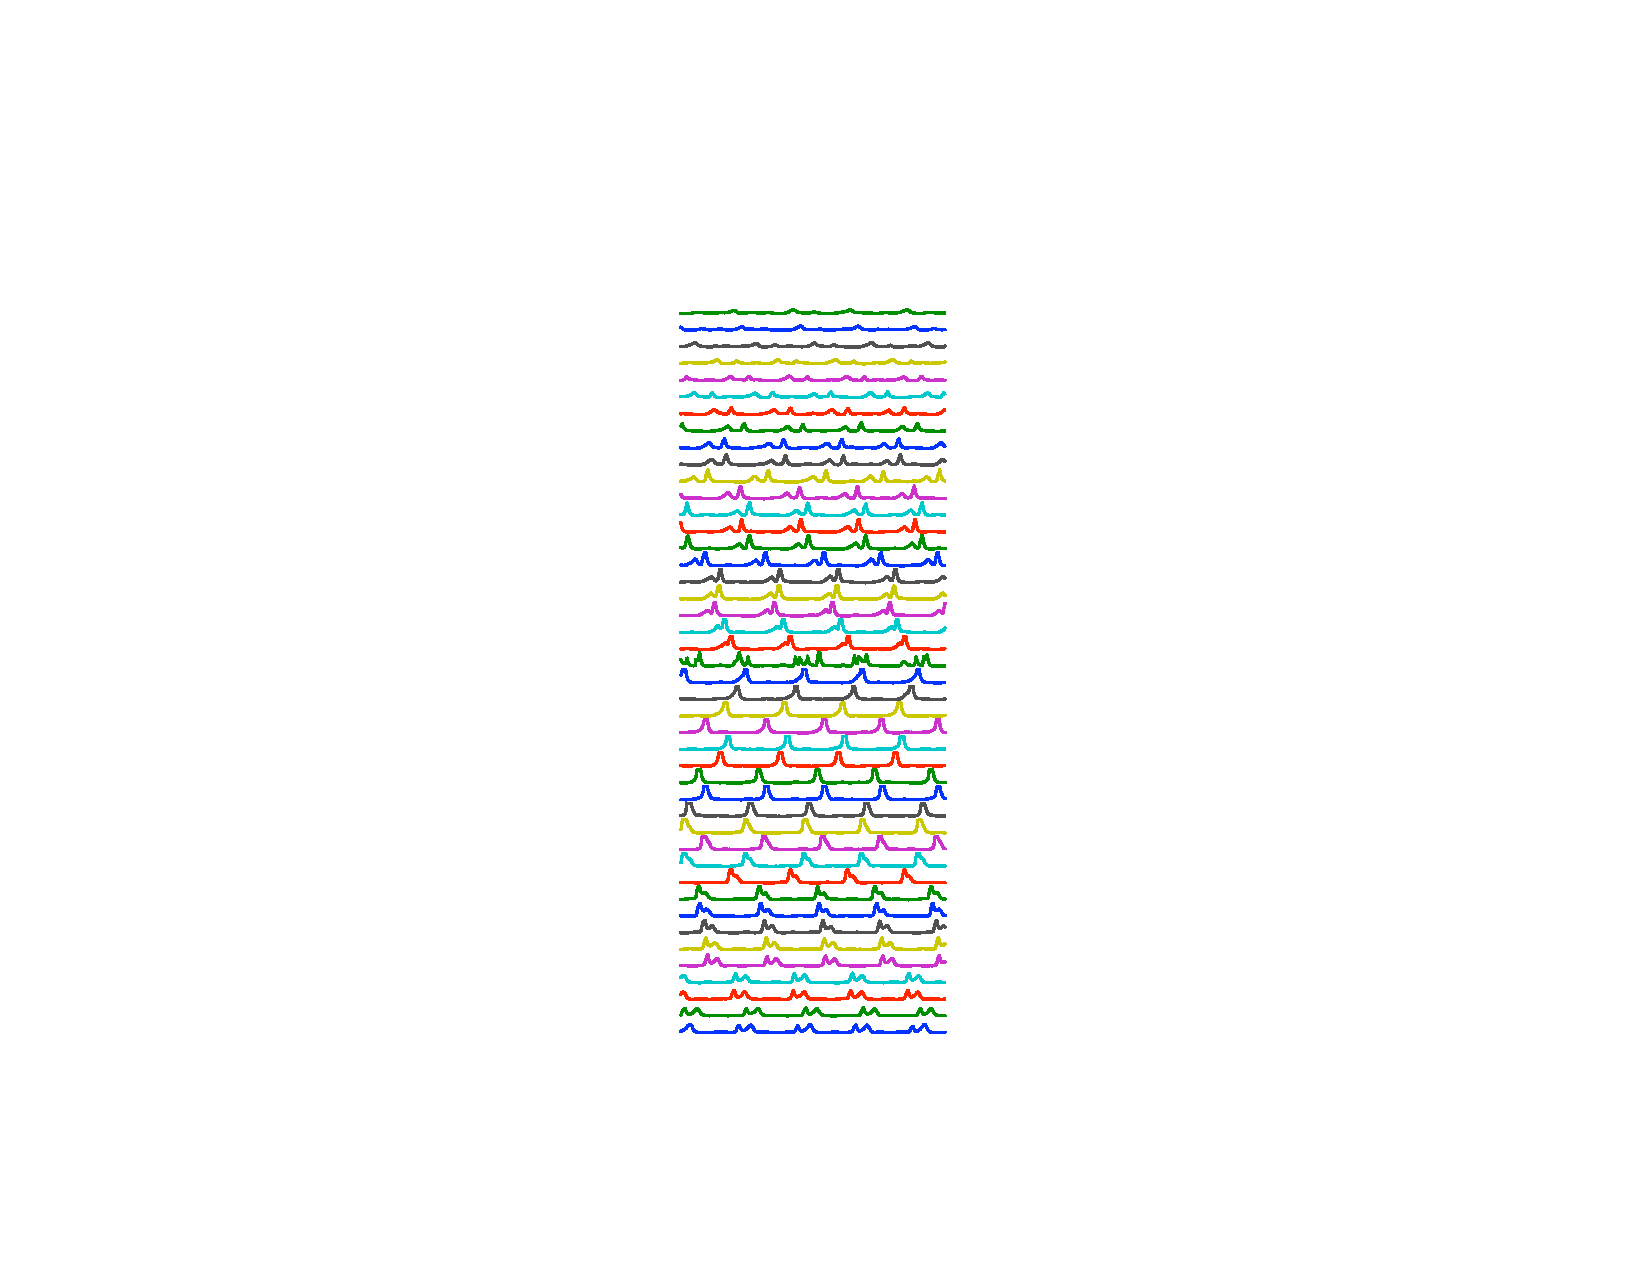
\includegraphics{all_splittingData}}
%\caption[Additional ]{\label{fig:alldata} 
%Spectrum analyzer data for }
%\end{figure}

%Also, I have data that I can analyze to examine the feasibility of a Chu lock. I recorded 999 traces that showed the output of the spectrum analyzer, the current and the voltage. I recorded these over several hours, during which the laser drifted into and out of good, single mode operation. In principle, this data could be analyzed. 

We have shown that we can change the rf oscillator frequency and thereby change the detuning. There are two limiting factors on the extent that we can do this. (Notice in Fig.\ \ref{fig:typicaldata} that the peaks get small as we continue to detune.) Both factors are geometrical in nature: First, the AOM diffraction efficiency decreases because the Bragg angle changes. Second, the diffraction angle changes, leading to a misalignment of the injected beams and a weakening of injection. However, even for large detunings, the injection lock can be achieved simply by realigning the output beams. We demonstrated this by successfully tuning the AOM driving frequency to the point where injection was lost, realigning (using the lasers as photo diodes) and then re-achieving successful injection lock.

\section{Summary and future work}
To summarize: I have built a laser system capable of driving stimulated Raman transitions between the $F=4$ and $F=5$ hyperfine levels of $^{87}$Sr$^+$. I successfully tuned and stabilized the master laser. Using an AOM, I generated two shifted beams that I used to injection lock two other lasers (slave 1 and slave 2).
%linewdith?

In order to ensure that the 408 nm 5 GHz detuned laser system works, we will need to actually drive stimulated Raman transitions in $^{87}$Sr$^+$. Completion of this requires the completion of the LVIS and other parts of the experiment. Getting the transition rate right will also likely require tweaks to many of the parameters of the current system. There are also additional optics that need to be installed to get the beams produced by this laser system to the atomic chamber. We will need to split the beams and then install optics to control their phase. 

The 408 nm 5 GHz detuned laser system could be improved in many ways. One thing that would be a great benefit is to increase the amount of time that the laser can operate without mode hopping. There was a technique described in Ref.\,\cite{chiowChuLock} for improving the stability of an ECDL by creating a closed feedback loop to monitor and minimize the laser's amplitude noise. I developed some circuitry and took some data to investigate a variation on this which could potentially be applied to injection locked lasers, but this is not included in this thesis. 




\appendix
\bibliographystyle{phBYU}
\bibliography{mybib}
 
\chapter{Measuring Beam Waist}
\label{BeamWaistAppendix}

Sometimes it is important to measure the waist of one's laser beam. For example, these techniques were useful when doing the work described in Section\,\ref{optimbeamWaist} to make sure that the maximum intensity of the beam was not above a certain threshold. In this appendix, I will discuss two methods for trying to characterize the profile of the laser beam. One involved a knife and did work. The other involved a camera and did not work due to the limitations of the camera.  

\section{Knife measurements}
In order to take measurements with a knife, we block some fraction of the beam by mounting the knife on a translation stage. We then use the translation stage to move the knife perpendicular to the direction of beam propagation. At several different positions, we look at the amount of power from the beam hitting a photo diode that is placed downstream from the knife. 
\begin{figure}
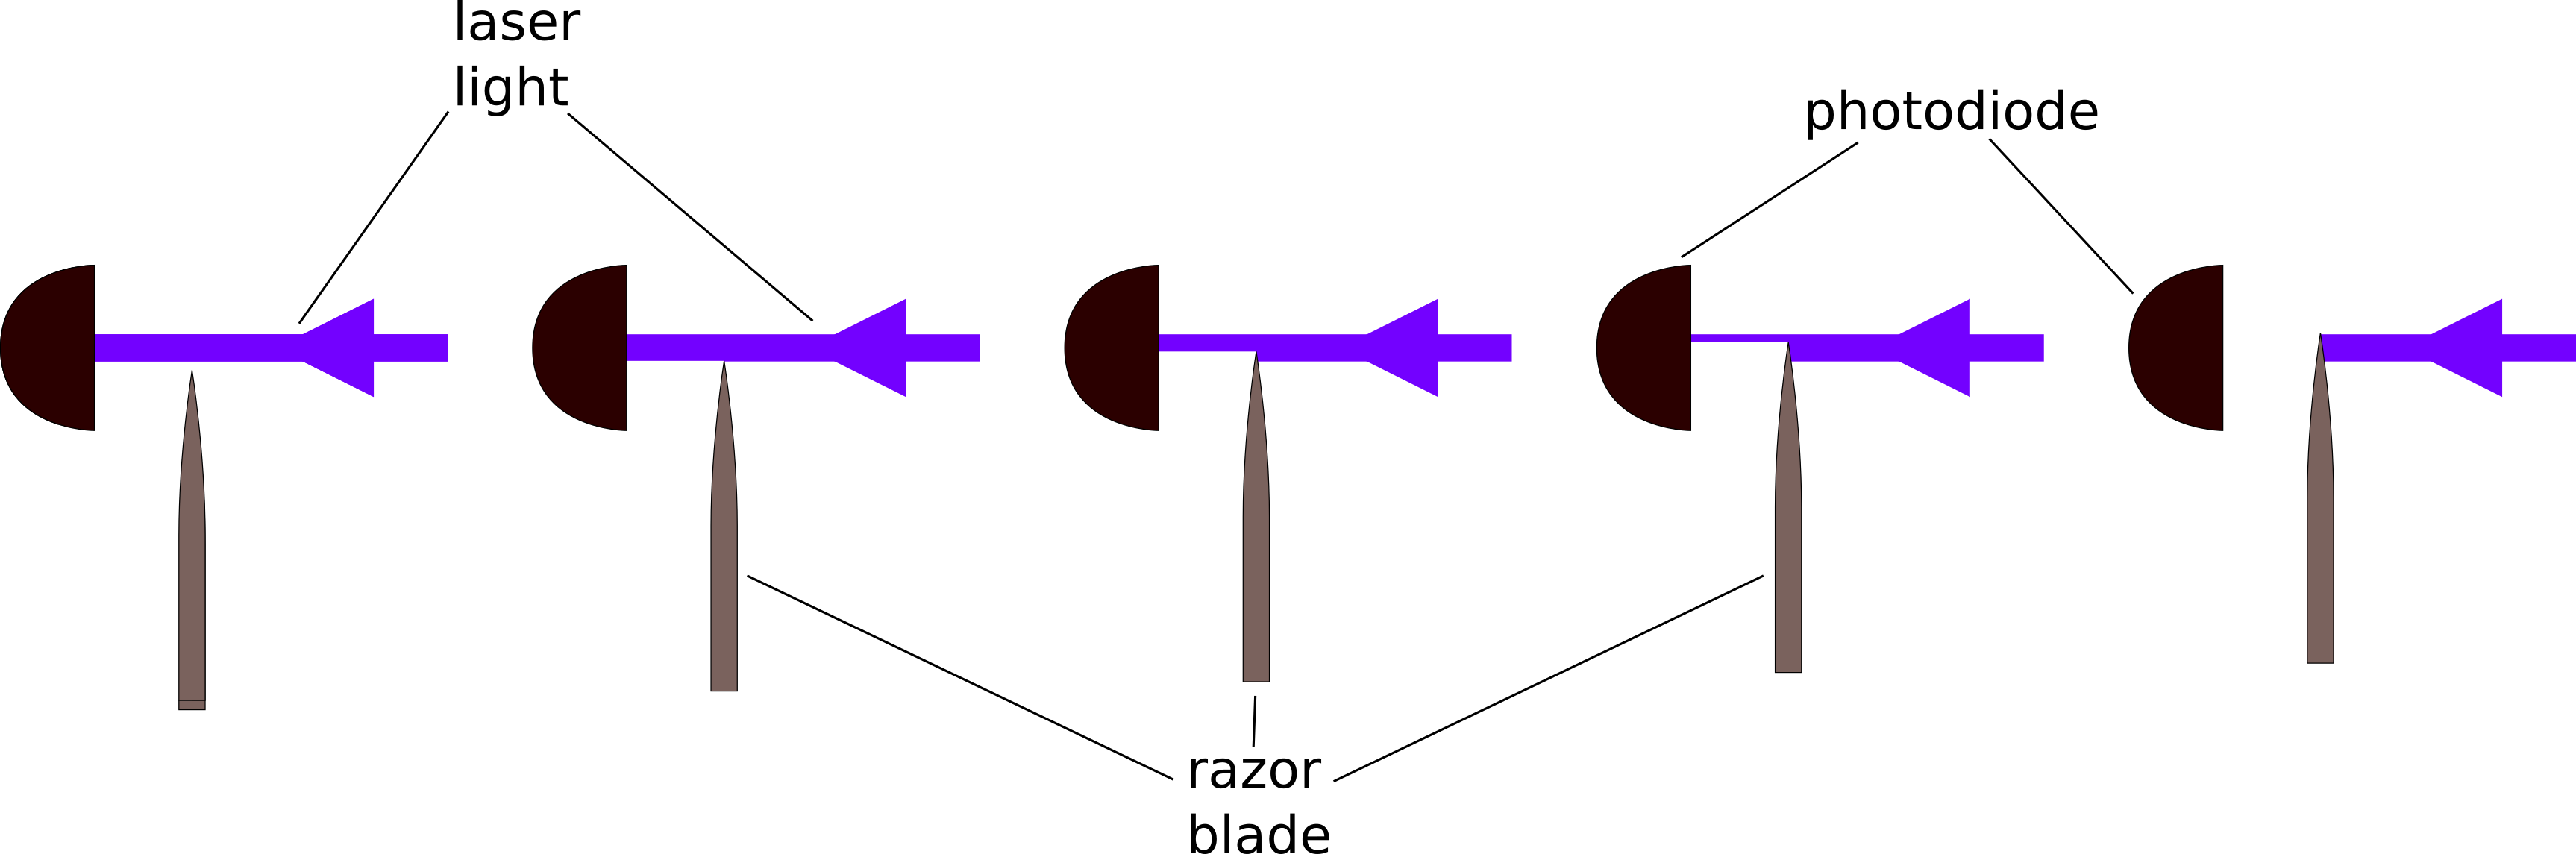
\includegraphics[width=.95\textwidth]{knife_drawing}
\caption[Knife diagram]{\label{knifeDiagram} An illustration of the razor blade method for measuring beam radius.
}
\end{figure}

If, for example, the knife is mounted vertically, the the knife would be moved in the horizontal direction. For each horizontal position, a different fraction of the beam would be occluded. The measurements on the photo diode correspond to the total power in the beam from $x=-\infty$ to $x_0$ where $x_0$ is the location of the knife. Thus, if we plot this power as a function of the spatial position of the knife, we expect that the result should be 
\begin{align}
P(x_0)&=\int_{\infty}^{\infty}\int_{-\infty}^{x_0} \frac{2 P}{\pi w_x(z) w_y(z)}\exp \left(-2\frac{x^2}{w_x^2(z)}-2\frac{y^2}{w_y^2(z)}\right) dx dy\\
P(x_0)&=\frac{P}{2} \left(\erf \frac{\sqrt{2} x}{W_x}+1 \right).\label{powerfitfun}
\end{align}
Eq.\,\ref{powerfitfun} can now be used as a function to which we can fit our measured data. 
%The code in masterFILEhoriz14Nov.m calculates the approximate beam waist based on a series of knife cuts. First, one loads the intensity (in arbitrary units) and the position (in the units that the waist will ultimately be given in) into a number of arrays named x1, x2, .. . etc. The user types the position of the knife along the waist (show picture) into the vector called positions. 

I wrote a function called ``d4sigma'' that attempts to calculate the second moment width using just the raw data. This is notoriously inaccurate because of how D4$\sigma$ is \emph{more} sensitive to radiation far from the center of the beam. Also, the knife technique lends itself to getting data of relatively low resolution. Finally, because I realized this and decided not to use the d4sigma function, the d4sigma function itself is not well-debugged and may be off by a constant factor.

This explains the exact method we use. The profile for the intensity of a Gaussian beam is given by
\begin{equation} \label{electricFieldExplicitForm}
I(r,z)=I_0\left(\frac{w_0}{w(z)}\right)^2 \exp \left(\frac{-2 r^2}{w^2(z)}\right)
\end{equation}
Extrapolating this to when there are two different waists in different directions, we get: 
\begin{equation}
I(r,z)= I_0\exp \left(-2\frac{x^2}{w_x^2(z)}-2\frac{y^2}{w_y^2(z)}\right) . 
\end{equation}
Now, total power ($P$) can be obtained by integrating the the intensity: 
\begin{align}
P&=\int_{-\infty}^{\infty}\int_{-\infty}^{\infty} ({\rm constants}) \exp \left(-2\frac{x^2}{w_x^2(z)}-2\frac{y^2}{w_y^2(z)}\right) dx dy\\
P&=\frac{\pi}{2} I_0 w_x(z) w_y(z).
\end{align}
The equation for $I_0$ takes the form
\begin{equation}
I_0=\frac{2 P}{\pi w_x(z) w_y(z)}.
\end{equation}
The symbol $I_0$ represents the maximum intensity that occurs within the beam (i.e. when $x=y=z=0$, or in other words, at the center of the narrowest part of the beam.)


The program instead calculates the second moment width and the beam waist exclusively by assuming the beam profile is Gaussian and finding parameters that will fit the measured data points to the function that we would expect if we were measuring the profile of a Gaussian beam. The function we fit to is contained in the file beamWaistCalculator, which takes as its arguments the raw position data and the raw intensity data. This function is 
\begin{equation}\label{fiterfeqn}
f(x)=a_1 \erf \left(\frac{x-a_3}{a_2}\right)+a_4.
\end{equation}
The function defined in ``beamWaistCalculator'' thus returns a vector containing $(a_1, a_2, a_3, a_4)$. Thus, to get the beam waist, we will take $a_2$ and multiply by $\sqrt{2}$. 

According to Siegman \cite{SiegmanBeamQuality}, the second moment width always propagates according to this equation: 
\begin{equation}
W_x^2(z)=W_{0x}^2 + M_x^4 \left( \frac{\lambda}{\pi W_{0x}}\right)^2 (z-z_{0x})^2. 
\end{equation}
Of course, for a Gaussian beam, we recognize that allowing $M_x^2\rightarrow 1$ gives us the equation for how the waist changes as it propagates. 

This program then tries to fit to this:
\begin{equation}
W_x=a_1 \sqrt{1+\left(\frac{(x-a_2) \lambda}{\pi a_1^2}\right)^2}\label{eq:Aafinder}
\end{equation}
and this:
\begin{equation}
W_x=a_1 \sqrt{1+(1+a_3^2) \left(\frac{(x-a_2) \lambda}{\pi a_1^2}\right)^2}.\label{eq:AAAfinder} 
\end{equation}
Eq.\,\ref{eq:Aafinder} is very similar to Eq.\,\ref{eq:AAAfinder} except that in Eq.\,\ref{eq:Aafinder}, we are effectively forcing $M^2$ to be one. As explained in Section,\ref{optimbeamWaist}, the assumption that $M^2=1$ is a useful one since, given a set of beam radius measurements for various points along the beam, the maximum intensity calculated assuming that $M^2=1$ will always be greater than or equal to the actual intensity of the beam for any possible actual value of $M^2$. Thus, for the purposes of verifying that the intensity that we measure and calculate is below the damage threshold of the AOM, we can use the values obtained with the assumption that $M^2=1$. 

Furthermore, because the beam radii/second moment widths used to perform the curve fit described in Eqs\,\ref{eq:Aafinder} and \ref{eq:AAAfinder} were calculated assuming the beam profile is Gaussian, we do not expect to get a very good estimate of $M^2$. This is all illustrated for one laser width in Fig.\,\ref{waistGraphs}.

\begin{figure}
\centering
\begin{subfigure}[b]{0.47\textwidth}
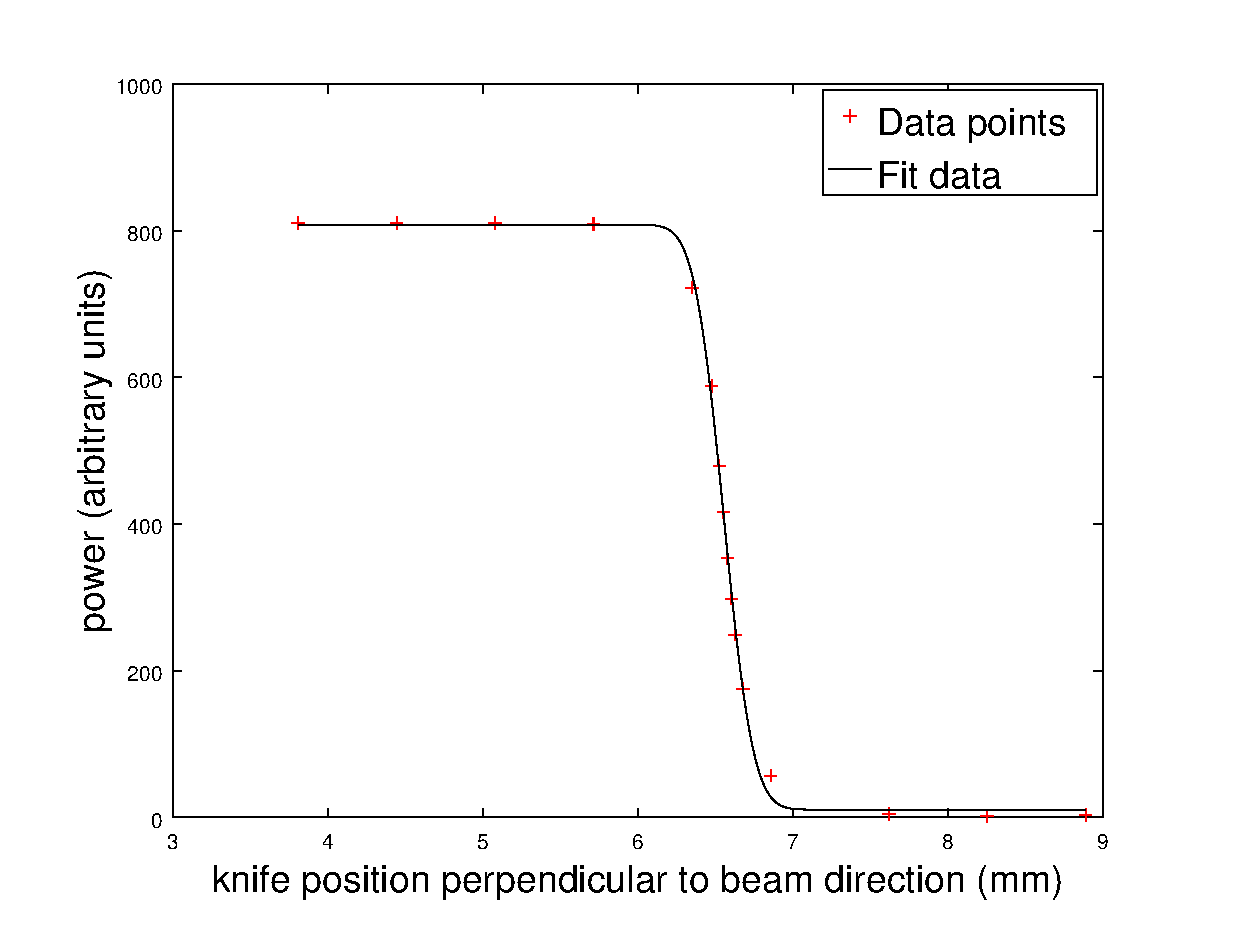
\includegraphics[width=1\textwidth]{waistFitExample.eps}
\label{waistFitExample}
\end{subfigure}
\begin{subfigure}[b]{0.47\textwidth}
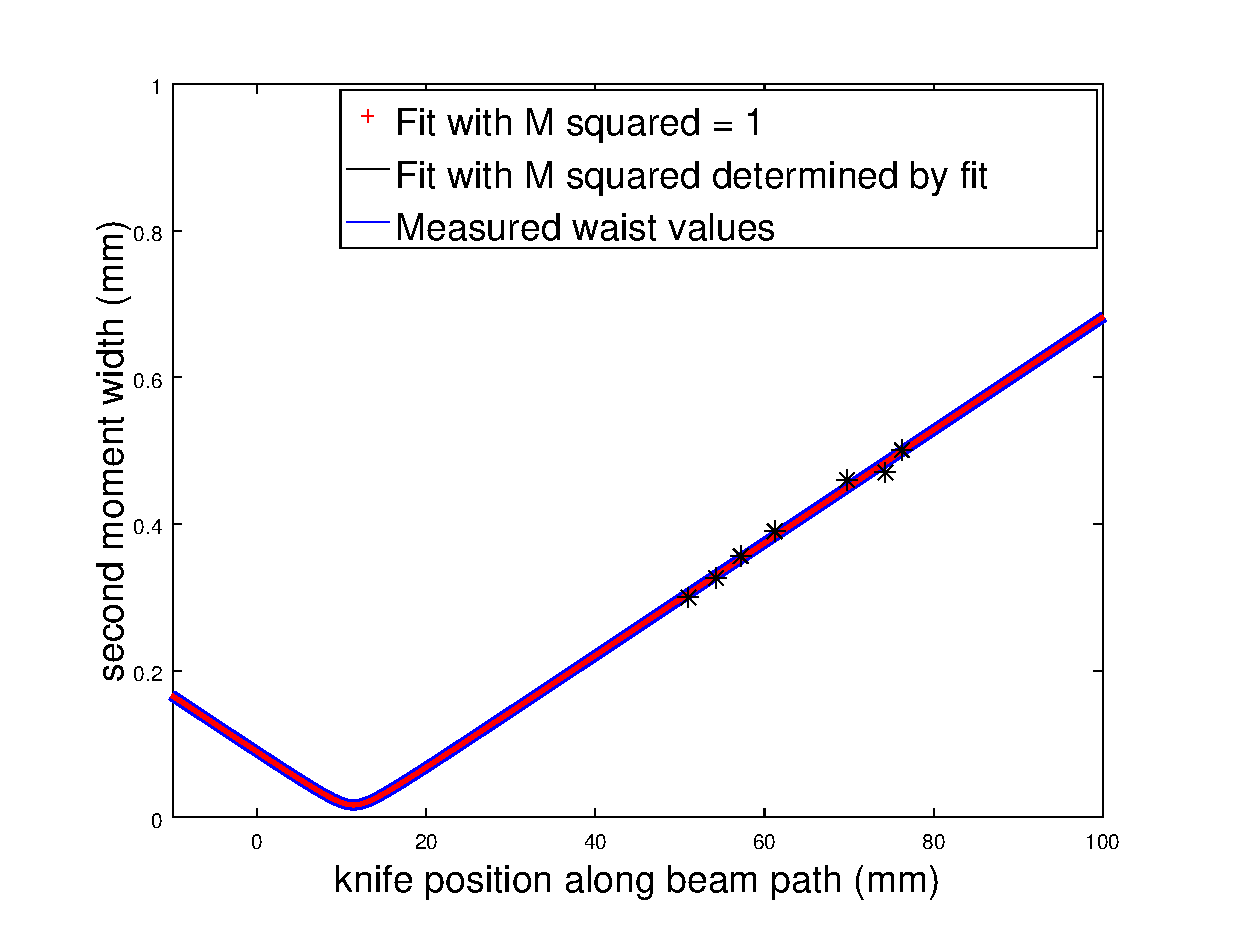
\includegraphics[width=1\textwidth]{waistExample.eps} 
\label{waistExample}
\end{subfigure}
\caption[Waist determination using a knife]{\label{waistGraphs} 
%Waist determination using a knife. On the left, there is typical data taken from a photodiode using a knife to occlude part of the beam. In general, we take data at several points along the beam path. This data is then fit to a function of the form shown in Eq.\,\ref{fiterfeqn}. This is shown on the right. The graph on the right shows a fit to equations of the form shown in Eq.\,\ref{eq:Aafinder} and \ref{eq:AAAfinder}. This data was taken for the $y$ direction on the beam going into the AOM. The fit values turn out to be $a_1=0.016875$ and $a_2=11.400$ for Eq.\,\ref{eq:Aafinder} and $a_1=1.6875e-2$, $a_2 = 11.4$, and $a_3=-2.6737e-7$ for the coefficients in Eq.\,\ref{eq:AAAfinder}. The value of $a_3$ is very small, which would suggest that $M^2\approx1$. However, because of the limited resolution and the fact that we fit the data points to a function before trying to calculate $M^2$ rather than using the directly-calculated second-moment width, we probably cannot trust the fit value corresoponding to $M^2$. On both graphs, the 0 mm point is arbitrary.
Waist determination using a knife. On the left is an example of data that was collected by measuring the beam power while occluding the beam in one direction using a razor blade. Each position on the x axis of the chart on the left corresponds to a different location of the razor blade within the beam. The curve fit to Eq.\,\ref{fiterfeqn} is also shown in the graph.
The graph on the right shows second moment widths of the beam at several points along the direction of propagation. The fit to Eqs.\,\ref{eq:Aafinder} and \ref{eq:AAAfinder} is also shown. 
The values of the coefficients found by fitting for the data shown turn out to be $a_1=0.016875$ and $a_2=11.400$ for the coefficients in Eq.\,\ref{eq:Aafinder} and $a_1=1.6875e-2$, $a_2 = 11.4$, and $a_3=-2.6737e-7$ for the coefficients in Eq.\,\ref{eq:AAAfinder}. The value of $a_3$ is very small, which would suggest that $M^2\approx1$. However, as mentioned in the text, I do not believe that this gives a very reliable estimate of the actual value of $M^2$. The x axis of both graphs is measured relative to an arbitrary point that was selected based on experimental convenience.
%The razor blade is mounted perpendicular to the direction of beam propagation. Each position on the x axis of the chart on the left corresponds to a different location of the razor blade within the beam. I took data like this for several positions along the direction of propagation of the beam. I then performed a fit where the fit function is of the form shown in Eq.\,\ref{fiterfeqn}. From the parameters generated by the curve fit, I extract an effective beam waist. Beam waists found in this way for several locations of the beam are shown in the plot on the right. The waist data as a function of distance along the path propagation is fitted to Eqs.\,\ref{eq:Aafinder} and \ref{eq:AAAfinder}. Allowing 
}
\end{figure}
%power arbitrary units might be milliamps.
%it is better to get it on both sides

\section{Using the camera}
We initially wanted to measure the $M^2$ of our beam. The measurements are hard to do accurately. We tried to use the camera and got results that were not entirely usable.

\subsection{Investigation of feasibility of using the camera}

The camera seems like an appealing device to use to measure beam parameters since it can take large amounts of 2D data quickly.

%insert plot of pixel count vs whatever? eh, maybe.

To investigate the camera's feasibility, we wanted to verify that the camera was (a) linear and (b) that each pixel reading was independent of the rest of the image. To this end, we took several images of the same beam, which we attenuated using the polarizing beam cube/wave plates adjustable attenuator setup described in Appendix\,\ref{twoWaveplateTrick}. We took 20 measurements. Each time we measured the total intensity of the beam using a photo diode and we took a corresponding image of the beam. Several example images are shown in Figure\,\ref{cameraimageexample}.

\begin{figure}
\centerline{
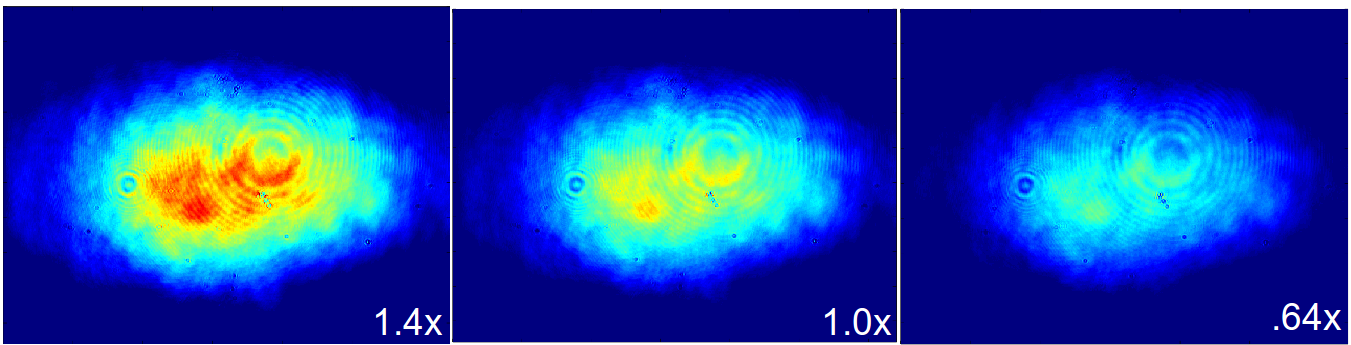
\includegraphics[width=0.95\textwidth]{cameraimage}
}
\caption[Sample camera images]{Three images taken using the camera. Each was the same laser beam with the attenuation adjusted using our wave plate and polarizer setup. The total power was measured using a photo diode and the relative total power is shown in the lower right corner of each image. By comparing the pixel values of similar spots within the image, we were able to bootstrap some calibration parameters for the camera. \label{cameraimageexample}}
\end{figure}

Our idea was that, if the camera is linear and the pixels act independently, the following statements should be true: 
\begin{itemize}
\item The ratio of the reading on any pixel to the reading on the same pixel in a different image should be equal to the ratio of the total power of the two beams used in the two readings as measured by the photo diode. 
\item Any two pixels reporting the same number of counts are experiencing the same radiance.
\end{itemize}

Thus, for example, if we see that the pixel located at $(214,442)$ has a pixel count of 127 in image 15, on which we measured the intensity to be proportional to 85.350, then we assume that we can compare it directly to a pixel located at the same location $(214,442)$ on image 20 (which had an intensity proportional to 119.70). If the reading from the $(214,442)$ pixel on image 20 was 155.46, we assume that a pixel count of 155.46 corresponds to $119.70/85.350=1.4025$ times as much intensity as a pixel count of 127. Additionally, we assume that any pixel we find in any of the images that reports a reading of 155.45 will have the same intensity as any other. 

We went through the 20 images like this: We selected some reference pixel. We then added that pixel to a master list. We then found the corresponding pixels in the other images whose position on the grid match that of the reference pixel. They were then added to the master list, making note of their position, the reading on the pixel (count) and the assumed ratio between the amount of light hitting that pixel and the amount of light hitting reference pixel as inferred based on the readings from the photo diode.

Then, we select a random pixel from the master list and look for other pixels that have the same number of counts within any of the images. If a pixel has the same reading (number of counts) as the randomly selected pixel in the master list, it is added to the master list. Since this new pixel has the same counts as the randomly selected pixel, we assume that the pixels have the same radiance relative to the reference pixel. Once the new pixel is added to the master list, we find the corresponding pixels from the other images and add them to our list. We assume that the true irradiance at these pixels is proportional to the irradiance of pixel we just added. 

In this way, we create a very long list of pixels, their counts and what we have inferred about the incident illumination of each pixel by comparing it to (a) other pixels that read the same value and (b) pixels in other images of different intensities. Note that the pixels in the list are not unique. Pixels can appear multiple times in the list.

If we plot the expected pixel count (as calculated by taking the reading on the main reference pixel and multiplying it by the relative radiance factors that we've been tracking) vs the actual pixel count, we get the plot in Fig.\,\ref{cameraPixelFit}, which seems to validate the assumption of pixel independence.

However, as one can see, the camera actually has a minimum threshold below which it does not report light very well. Because the camera throws away information and has a minimum intensity threshold to register, we throw out any $M_{i j}=0$. This way our function doesn't get penalized for showing a non-zero intensity for pixels that read out zero. The number of $M_{i j}=0$ obviously doesn't change as we try different iterations of $f(M_{ij})$, so there's no way to game our little metric to make it not work.
%We did a standard fit to a 4th order polynomial and got a reasonable function to correct for the pixel values. We were a little worried about bias in the selection of pixels and things like that. We wasted some time trying to figure out how to do this better. 

We performed a curve fit to model our pixels response. In order to do this, we had to devise a cost function that produces some figure of merit to tell us whether our test function is succeeding at making all of the pixels have the right ratio. The way it works is this: Suppose that $M_{i j}$ is a big list of our pixels. The variable $j$ runs from 1 to 20, corresponding to the 20 different images, while $i$ represents all the pixels in our image.\footnote{Thus, if we are analyzing 8x8 bins, we should have 480/8*640/8=4800 pixels and i will range between 1 to 4800} Let $f(p)$ be the proposed function that takes as its argument the count on a given pixel and gives as its output something that scales with the actual intensity of the light. The figure of merit that we can use to optimize $f(p)$ is calculated as follows: 

\begin{equation}\label{fom}
{\rm Figure\:of\:merit}=\sum_{ M_{i j}\neq 0}\left(\frac{f(M_{i j})/P_j}{{\rm average\,of\,all\,nonzero\,} f(M_{i j})/P_j {\rm \,for\,the\,ith\,pixels}}-1\right)^2
\end{equation}

where $P_j$ is the power of the j th image.

In words, Eq.\,\ref{fom} can be described as follows: First, act on the pixels with the proposed function. Then, scale them according to the intensity ratios (i.e. the i th pixel in image 1 gets divided by $P_1$ while the i th pixel in image 3 gets divided by $P_3$). Then, see by what fraction the intensity of that pixel differs from the average of the intensities calculated using data from the pixels corresponding to that one. If the function really were to find the ratio perfectly, then $f(M_{ij})/P_j$ should be exactly the same for the i th pixel from each of the j images. 


We used this function to calculate what correction function to use. We did a couple of them and found great agreement with the inversion of the previous function--thus suggesting that our previous method was acceptable. 


\begin{figure}
\centerline{
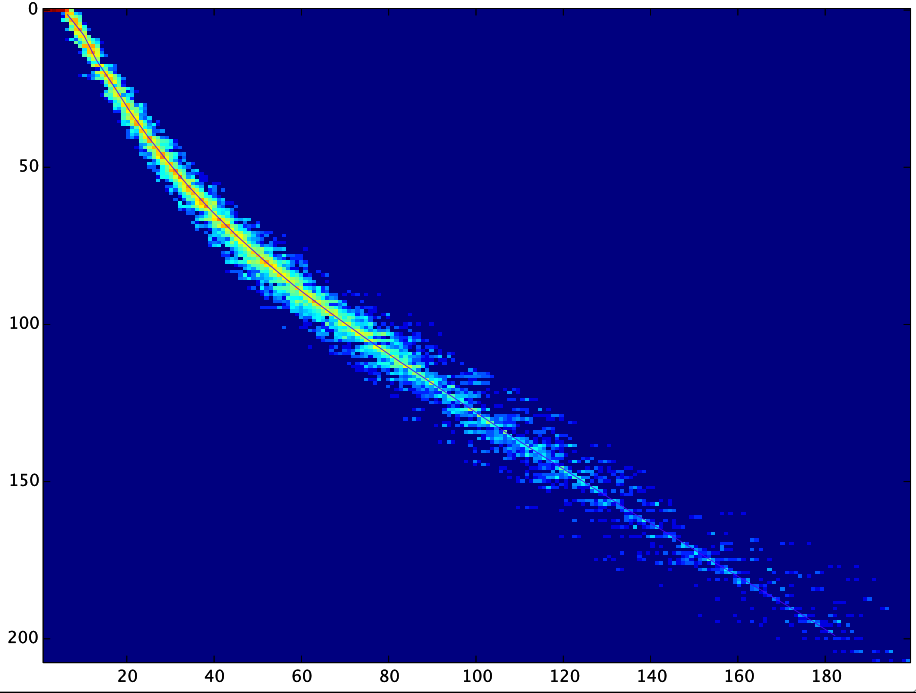
\includegraphics[width=0.95\textwidth]{cameraPixelFit}
}
\caption[Camera linearity and offset]{On the x axis is the inferred pixel reading based on our assumptions about the ratios of pixel readings. On the y axis, we can see the actual readings of the pixels. This illustrates clearly the threshold issue of the camera. In the top, left side of the plot, there is clearly a region where our inferred readings should be nonzero, but the actual readings on the camera remain at zero.\label{cameraPixelFit}}
\end{figure}

In the end, the camera offset and nonlinearity made it unsuitable for sensitive measurements of the second moment width of the beam. However they did provide a reasonable sanity check on our methods.
%\end{document}

\include{AppendixTryingtoFigureouttheChuLock}
\chapter{Calculation of Grating Ratio}\label{GratingRatioAppendix}
In order to narrow the linewidth of the master laser and make it more tunable and stable, we have mounted a diffraction grating in a Littrow configuration. The gratings are mounted on piezoelectric actuators that can be automatically moved in unison by our control circuitry. 

However, in order for this to work, it is important to verify that the piezos can be scanned in such a way that the resonances of the external cavity track smoothly. In order to accomplish this, one must find a ratio that relates the relative rates at which each piezoelectric actuator is scanned. 

Normally, this is not very tricky. However, at one point we discovered that for certain geometries, the appropriate ratio might be negative. To this end, we created the following Mathematica notebook to model the motion of the grating and help us to ensure that our electronics are capable of moving the actuators properly. 
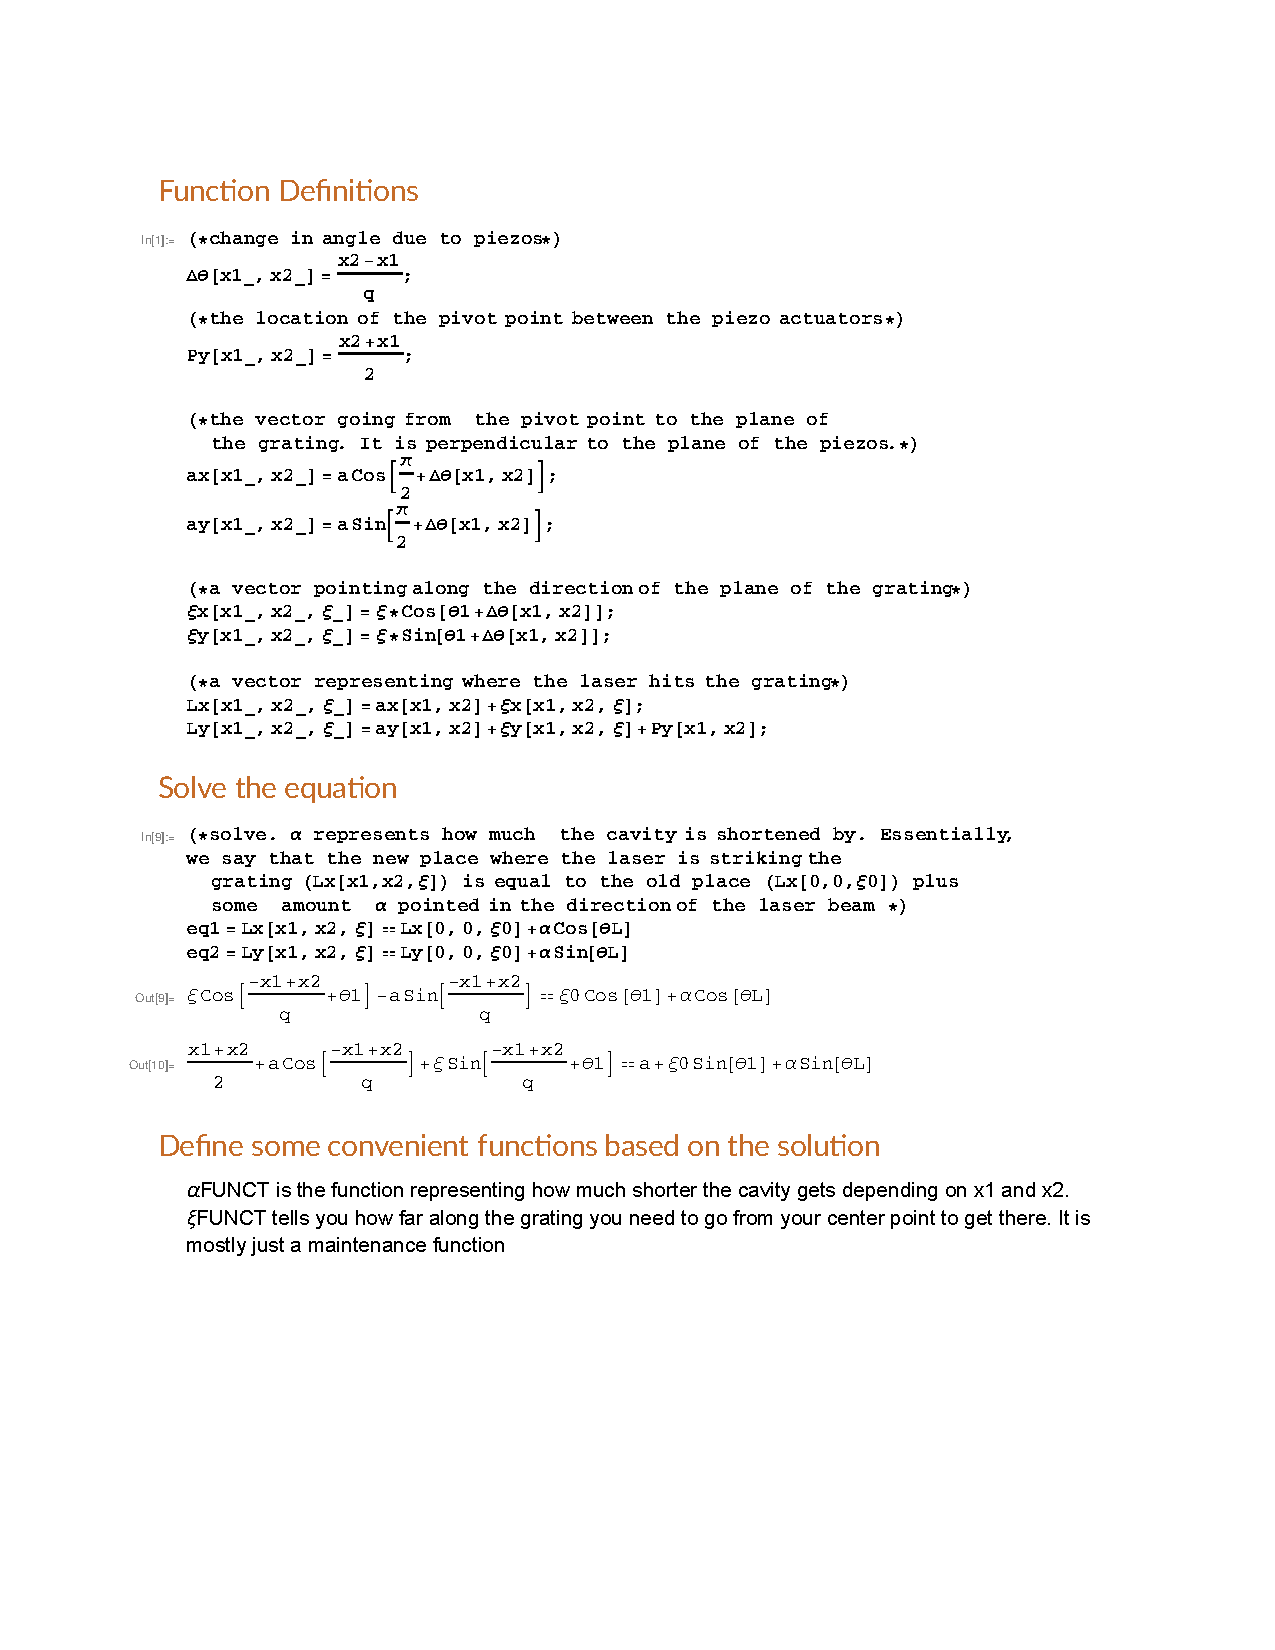
\includepdf[pages={1-10}]{grating_motion}



\section{Spectrum Analyzer}

The spectrum analyzer consists of a 10 cm cavity with two mirrors XXXXXXX FIND OUT WHICH ONES. 

One of the mirrors is mounted on a Thorlabs kinematic piezo mount and attached to a piezo driver designed specifically for spectrum analyzers.

The cavity is designed to be nearly semiconfocal\footnote{I used to think that this was because the transverse modes of a semiconfocal cavity overlap. However, it seems that a concentric cavity would be more likely to have this property. Oh wait. I get it. The semiconfocal cavity has all its transverse modes very small.} This is because the transverse modes of a semiconfocal cavity correspond to longitudinal modes with comparable lengths. This ensures that it is relatively easy to couple the laser to the cavity since we are relatively insensitive to which of the transverse modes we are coupling to. 

%\footnote{How do I know whether I'm semiconfocal for all practical purposes? I mean, somehow lower finesse should make me less sensitive to small variations in the cavity length. Furthermore, are there models where the errors never really go away? You know? I guess I mean where it doesn't just become part of the noise. I suppose chaos is one example of this--where arbitrarily high precision is needed to predict even the macroscopic behavior of the system. Is any aspect of this system chaotic?}

The alignment procedure was as follows:

The entry mirror was aligned so as to be retroreflecting the incoming beam. Later, The rear mirror was adjusted so that beam reflected back. 


\chapter{Adjustment of Light Amounts}

The light level from the master laser is constrained by our requirement that the Master laser operate single mode. However, we require control of the light levels further downstream in order to have the right light levels to avoid damage to the Acousto-Optic Modulator (AOM) and to have the right amount of light to injection lock the other lasers. 

A typical way to accomplish this is to install a half wave plate followed by a polarizing beam cube. In this way, one can take the linearly polarized incoming light and rotate its polarization to any angle. One can thus exert complete control of the amount of light coming out of the polarizing beam cube. 

We had initially intended to use this scheme. However, there was a mistake in placing the order. Instead of 0 order waveplates, we had received multi-order waveplates, whose performance rapidly degrades for wavelengths far from the specified wavelength. 

We could have easily ordered a 0 order waveplate to replace them. However, we found a way to use the exising wavelengths that was mildly interesting.

\subsection{A review of the principles of operation of a waveplate: }

Recall that a waveplate rotates polarization by changing the relative phase of the oscillating components of the incoming polarized light. A waveplate generally\footnote{and maybe always} has a fast axis and a slow axis. A half-wave plate is designed so that, at the specified wavelength, the component of polarization along the slow axis acquires a phase shift of $(2m+1)*\pi$ relative to the fast axis\footnote{here $m$ is an integer}. 

Recall that the phase acquired by light as it passes through a medium of index of refraction $n$ is given by 

\begin{equation}
  \Delta \phi = \frac{2 \pi n x}{\lambda} \label{deltaPhi0}
\end{equation}

Given indices of refraction of $n_1$ and $n_2$ for our two axes, we find that the difference in phase acquired by the components of the light's polarization will be 

\begin{equation}
\Delta \phi=\frac{2 \pi n_1 x}{\lambda} -\frac{2 \pi n_2 x}{\lambda}. \label{deltaPhi2}
\end{equation}

and we find that, in order to achieve the correct phase shift, the acceptable thicknesses of our half wave plate must satisfy

\begin{equation}
  \Delta \phi=(2m+1)\pi \label{deltaPhi1}
\end{equation}
where $m$ is the order of the waveplate.

Combining \ref{deltaPhi1} and \ref{deltaPhi2} we find that the thickness of a waveplate $x$ is given by

\begin{equation}
x=\frac{(2m+1) \lambda}{2 (n_1-n_2)}. \label{deltaPhi3}
\end{equation}


We now examine what will happen if we put a different wavelength than specified into the waveplate. Thus, we assume that $x$,$n_1$,$n_2$ and $m$ give the appropriate $\pi$ phase shift for the wavelength at which the waveplate is designed to work ($\lambda_s$). Now, we try light of a different wavelength, $\lambda'$. Assuming that the indices of refraction stay roughly the same for both $\lambda_s$ and $\lambda'$, we see that 

\begin{align}
\Delta \phi=\frac{2 \pi (n_1-n_2) x}{\lambda'} 
\end{align}
Then, taking $x\rightarrow ((2m+1) \lambda_s)/(2 (n_1-n_2))$ from Eq.\ \ref{deltaPhi3}, we get 
\begin{align}
\Delta \phi&=\frac{2 \pi (n_1-n_2) (2m+1) \lambda_s}{2 (n_1-n_2)\lambda'} \\
\Delta \phi&=\frac{\pi (2m+1) \lambda_s}{\lambda'} \label{deltaPhi4}
\end{align}
Eq.\ \ref{deltaPhi4} illustrates that the performance of a multi-order waveplate (with high value for $m$) will degrade more rapidly at different wavelengths than a low-order waveplate. 

In our lab, we had a half wave plate, but it was a multi-order plate designed for 405 nm. Thorlabs specifies that the waveplates we had\footnote{I know, put which ones exactly} will provide the correct retardance at 405 nm, however they also specify that at 407.71 nm the net retardance is 0.3655746 waves, or $\Delta \phi=(m_2+.3656) (2 \pi)$. Based on Eq.\ \ref{deltaPhi4}, we see that this is consistent with and $m=55$ order waveplate. 

The problem here is that, in order to completely control the amount of light getting to the AOM, we want to change the polarization from fully vertical to fully horizontal. Given that the incoming light is vertically polarized, this retardance does not allow us to get fully horizontally polarized light, thereby imposing a minimum amount of light on us, which was not welcome. 

However, we found that we can compensate for this by merely using two waveplates in series. Using numerical methods, we found that the user can fix the orientation of one of the waveplates in such a way that by rotating the other waveplate over some reasonable distance \footnote{i.e. over a range of angles large enough that rotating the waveplate by hand gives the user a decent amount of control}, the outgoing light can be made to smoothly transition between being completely vertical or completely horizontal\footnote{Though the states in between can be made to have any combination of horizontally polarized and vertically polarized light, the light that comes out in these states are not necessarily linearly polarized}

This can be demonstrated using the Jones matrix formalism. The polarization of the incoming light can be represented by the following Jones vector: 
\begin{equation}
\begin{pmatrix}
0\\1
\end{pmatrix}
\end{equation}

The Jones matrix corresponding to our waveplate is easily derived. Given the : 

\begin{multline}
\begin{pmatrix}
\cos\theta & - \sin \theta \\
\sin \theta & \cos\theta \\
\end{pmatrix}
\begin{pmatrix}
\xi & 0 \\
0 & 1 \\
\end{pmatrix}
\begin{pmatrix}
\cos\theta &  \sin \theta \\
-\sin \theta & \cos\theta \\
\end{pmatrix} \\
=
\begin{pmatrix}
\cos ^2 \theta+\xi \sin^2 \theta &  \cos\theta \sin \theta-\xi \cos\theta \sin \theta \\
\cos\theta \sin \theta-\xi \cos \theta \sin\theta & \xi \cos^2 \theta + \sin^2 \theta \\ \label{JonesMatrix001}
\end{pmatrix}
\end{multline}

where $\theta$ is the angle between the fast axis and the x axis. 

We let $\xi\approx e^{.366 (2 \pi)}$ as specified by the waveplate. Then, to represent two of them mounted at angles $\theta_1$ and $\theta_2$ respectively, we need merely multiply two matrices like the one in Eq.\ \ref{JonesMatrix001}. Writing out the result is simple, but probably not overly enlightening. 

By numerical experimentation, we found that there was a set of angles where we could mount our two waveplates that would result in a polarization for the outgoing light that is orthogonal to the polarization of the incoming light. 

\begin{figure}
    \centerline{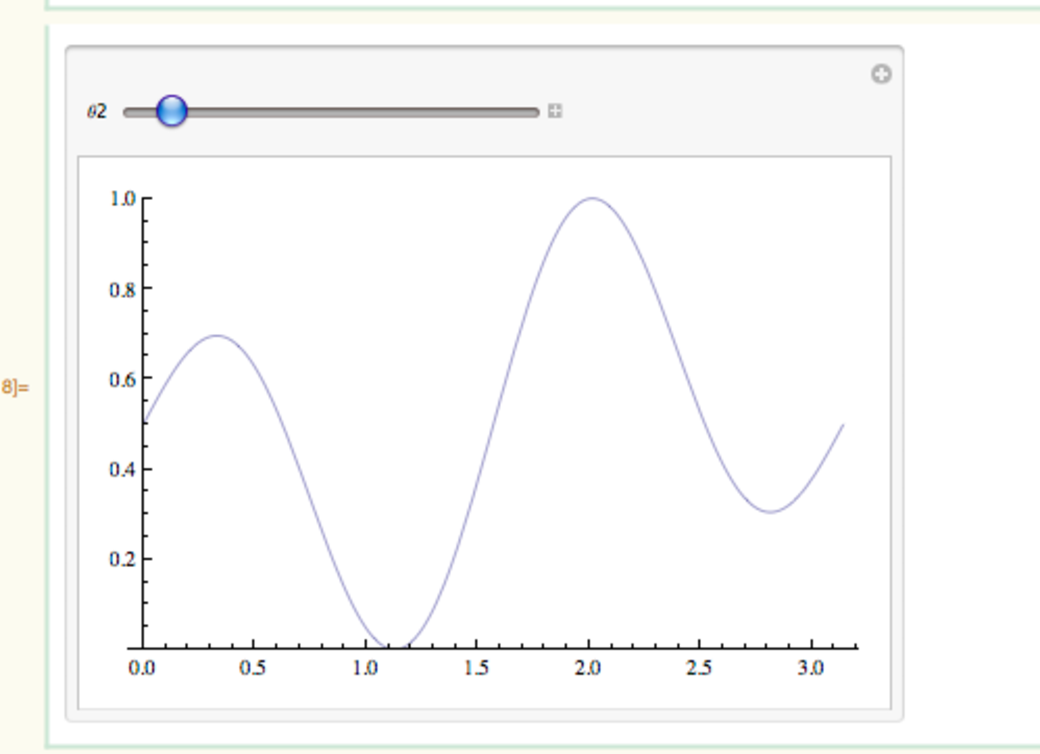
\includegraphics{numericalMethod}}
    \caption[Numerical method]{\label{fig:numericalLightControlMethod}
    Just plot the magnitude of the vertically polarized component as a function of $\theta_1$. I used the slider to control $\theta_2$. Obviously, I'll illustrate this better at some point.}
\end{figure}

We found that when we mount one of the waveplates at angle XXXX, we can adjust the vertical component of the polarization of the outgoing light to anywhere between 0 and one as we adjust it from angle XXXX to YYYY. We did this numerically. 

By physical and numerical experimentation, we found that you can achieve these angles by subsequently adjusting each of the two waveplates in turn. Keeping 100\% of the light vertically polarized is easy and can be achieved for any fixed value of $\theta_2$ since $\theta_1$ can simply be adjusted so that the fast axis of the first waveplate aligns with the slow axis of the second. In this way, the total phase shift experienced by all the components is equal.

Thus, to correctly place the second waveplate at the angle  $\theta_2$, we adjust both angles until the outgoing light is entirely horizontally polarized (as measured by the output of the polarizing beam cube). I found that mounting the waveplates at the approximate angles I calculated followed by alternately adjusting each waveplate to minimize the amount of light transmitted achieved the desired result. 

There is some intuition to be had here. One thing I noticed was that, when the waveplates are adjusted so that the outgoing light is horizontally polarized, the magnitude of the components of light in each polarization between the waveplates is equal. This suggests some symmetry. 

%Consider that, in this part of the setup, we have a time-reversal symmetry. What I mean is, if we send the outgoing light in backwards, we get the incoming light going backwards. Now, I am going to, at some future point write about the following: 

If you have two components of polarization--a horizontal and a vertical with some phase $\phi$ between them, the time reversed wave will have a phase $-\phi$ between its horizontal and vertical components. 

Now, consider the light travelling between the two waveplates (after going through waveplate \#1 but before going through waveplate \#2). 

We first select a rather unusual basis in which to express the Jones vector of this light. We will use the respective polarization vectors of the incoming light and the outgoing light as my basis vectors. These vectors may be non-orthogonal, but they still span the space of all possible polarizations.  

Now, after passing through our first waveplate, the components of polarization as expressed in this basis will have some relative phase offset. 

Now, consider what this would look like time-reversed. If, for example, the phase of the component along the first direction of polarization had a phase $\phi$, the time reversal means that the other component of polarization will be ahead by a phase $\phi$. Now, this is the crux of the argument: 

Consider light with the second desired polarization being sent backwards into the second polarizer. By symmetry, we can orient the second polarizer such that the components of the light, when described in the basis comprised of our unit vectors that point along the directions of the respective fast axes of the two polarizing waveplates 


%maybe do it differentially? You know? 

%let it be imperfect. Use other time for cleverness. Take advantage of having idea net out. 
%should I find a commutator? 
%IDK if I did this right with my \xi
%don't forget to cite peatrossware
%http://www.thorlabs.com/NewGroupPage9.cfm?ObjectGroup_ID=713 is where I got the spreadsheet. 

%  \include{AppendixB}

 \phantomsection \addcontentsline{toc}{chapter}{Index}
  \renewcommand{\baselinestretch}{1} \small \normalsize
  \printindex


\end{document}
\grid
